\documentclass[]{ioereport}
\usepackage{algorithm}
\usepackage{algorithmic}
\usepackage{booktabs}
\usepackage{multirow}
\usepackage{graphicx}
\usepackage{array}
\usepackage{adjustbox}
\usepackage{tabularx}
\providecommand*{\algorithmautorefname}{Algorithm}
\newcolumntype{L}[1]{>{\raggedright\arraybackslash}p{#1}}


\includeonly{sections/declaration, sections/certificate, sections/acknowledgement, sections/abstract, sections/introduction, sections/literature, sections/feasibility, sections/theoretical, sections/mathematical, sections/methodology, sections/dataset, sections/implementation, sections/results, sections/appendix}

% \includeonly{sections/results}

\begin{document}

\newacronym{cnn}{CNN}{Convolutional Neural Network}
\newacronym{lstm}{LSTM}{Long Short-Term Memory}
\newacronym{2d}{2D}{2-Dimensional}
\newacronym{3d}{3D}{3-Dimensional}
\newacronym{gan}{GAN}{Generative Adversarial Network}
\newacronym{nerv}{NeRV}{Neural Representations for Videos}
\newacronym{nera}{NeRA}{Nerual Representations for Audios}
\newacronym{nerva}{NeRVA}{Nerual Representations for Videos and Audios}
\newacronym{ddvc}{DDVC}{Deep Discriminative Video Compression}
\newacronym{gpu}{GPU}{Graphics Processing Unit}
\newacronym{fps}{FPS}{Frames Per Second}
\newacronym{psnr}{PSNR}{Peak Signal-to-Noise Ratio}
\newacronym{db}{dB}{decibels}
\newacronym{mse}{MSE}{Mean Squared Error}
\newacronym{aws}{AWS}{Amazon Web Services}
\newacronym{html}{HTML}{Hypertext Markup Language}
\newacronym{css}{CSS}{Cascading Style Sheets}
\newacronym{lpips}{LPIPS}{Learned Perceptual Image Patch Similarity }
\newacronym{ssim}{SSIM}{Structural Similarity Index Measure}
\newacronym{fvd}{FVD}{Fréchet Video Distance}
\newacronym{uvg}{UVG}{Ultra Video Group}
\newacronym{hevc}{HEVC}{High-Efficiency Video Coding}
\newacronym{avc}{AVC}{Advanced Video Coding}
\newacronym{codec}{codec}{Coder Decoder}
\newacronym{cpu}{CPU}{Central Processing Unit}
\newacronym{inr}{INR}{Implicit Neural Representation}
\newacronym{bpp}{bpp}{bits per pixel}
\newacronym{rgb}{RGB}{Red Green Blue}
\newacronym{nvr}{NVR}{Neural Video Representation}
\newacronym{dct}{DCT}{Discrete Cosine Transform}
\newacronym{ecm}{ECM}{Enhanced Compression Model}
\newacronym{visqol}{ViSQOL}{Virtual Speech Quality Objective Listener}
\newacronym{cdpam}{CDPAM}{Contrastive Deep Perceptual Audio Metric}
\newacronym{pesq}{PESQ}{Perceptual Evaluation of Speech Quality}
\newacronym{stoi}{STOI}{Short-Time Objective Intelligibility}
\newacronym{knn}{KNN}{K-Nearest Neighbours}
\newacronym{svd}{SVD}{Singular Value Decomposition}
\newacronym{vvc}{VVC}{Versatile Video Coding}
\newacronym{nvc}{NVC}{Neural Video Coder Decoder}
\newacronym{kb}{KB}{kilobytes}
\newacronym{kib}{KiB}{kibibytes}
\newacronym{mb}{MB}{megabytes}
\newacronym{mib}{MiB}{mebibytes}
\newacronym{gb}{GB}{gigabytes}
\newacronym{gib}{GiB}{gibibytes}
\newacronym{bps}{bps}{bits per seconds}
\newacronym{kbps}{kbps}{kilobits per seconds}
\newacronym{mbps}{Mbps}{megabits per seconds}
\newacronym{siren}{SIREN}{Sinusoidal Representation Networks}
\newacronym{ptq}{PTQ}{Post-raining Quantization}
\newacronym{inn}{INN}{Implicit Neural Networks}
\newacronym{mlp}{MLP}{Multilayer Perceptron}
\newacronym{rbkd}{RBKD}{Response-Based Knowledge Distillation}
\newacronym{vae}{VAE}{Variational Autoencoder}
\newacronym{ide}{IDE}{Integrated Development Environment}
\newacronym{kld}{KLD}{Kullback-Leibler Divergence}
\newacronym{emd}{EMD}{Earth Mover's Distance}
\newacronym{pcm}{PCM}{Pulse Code Modulation}
\newacronym{fft}{FFT}{Fast Fourier Transform}
\newacronym{mdct}{MDCT}{Modified Discrete Cosine Transform}
\newacronym{crc}{CRC}{Cyclic Redundancy Check}
\newacronym{imdct}{IMDCT}{Inverse Modified Discrete Cosine Transform}
\newacronym{crf}{CRF}{Constant Rate Factor}
\newacronym{lsd}{LSD}{Log Spectral Distance}
\newacronym{sqnr}{SQNR}{Signal-to-Quantization Noise Ratio}
\newacronym{msqe}{MSQE}{Mean Squared Quantization Error}
\newacronym{lzma}{LZMA}{Lempel-Ziv-Markov chain algorithm}
\newacronym{webrtc}{WebRTC}{Web Real-Time Communication}
\newacronym{uml}{UML}{Unified Modeling Language} % input acronyms.tex file

\titlepreamble{A Major Project Report (Part-B)\\On}
\projecttitle{Data-driven Video Codec with Implicit Neural Representations}
\addauthor{Abhinav Chalise}{THA077BEI003}
\addauthor{Nimesh Gopal Pradhan}{THA077BEI026}
\addauthor{Nishan Khanal}{THA077BEI027}
\addauthor{Saugat Neupane}{THA077BEI043}
\supervisor{Er. Dinesh Baniya Kshatri}

\coverpage

\phantomsec

\coverpageB

% \section*{DECLARATION}
% \addcontentsline{toc}{section}{DECLARATION}
%     We hereby declare that the report of the project entitled \textbf{``\titlename"} which is being submitted to the \textbf{Department of Electronics and Computer Engineering, IOE, Thapathali Campus}, in the partial fulfillment of the requirements for the award of the Degree of Bachelor of Engineering in \textbf{Electronics, Communication and Information}, is a bonafide report of the work carried out by us. The materials contained in this report have not been submitted to any University or Institution for the award of any degree and we are the only author of this complete work and no sources other than the listed here have been used in this work.
% \\ \\ \\ \\
% \foreach \name [count=\i] in \authornames {
%     \foreach \roll [count=\j from 1] in \authorrollnumbers {
%         \ifnum\i=\j
%             \name\ (Class Roll No: \roll) \hrulefill \\ \\ 
%         \fi 
%     }
% }
% \\
% \textbf{Date:} \today
% Only change the name, Keep this section as it is
\section*{CERTIFICATE OF APPROVAL}
    The undersigned certify that they have read and recommended to the \textbf{Department of Electronics and Computer Engineering, IOE, Thapathali Campus}, a major project work titled \textbf{``\titlename"} submitted by \textbf{\authornames} in partial fulfillment for the award of Bachelor of Engineering in Electronics, Communication and Information. The Project was carried out under special supervision and within the time frame prescribed by the syllabus.
    
    We found the students to be hardworking, skilled and ready to undertake any related work to their field of study and hence we recommend the award of partial fulfillment of Bachelor of Engineering in Electronics, Communication and Information. \\
    
    \rule{0.5\linewidth}{0.4pt}\\
    Project Supervisor\\
    \supervisorname\\
    Department of Electronics and Computer Engineering, Thapathali Campus\\

    \rule{0.5\linewidth}{0.4pt} \\
    External Examiner \\
    Er. \\
    Department of Electronics and Computer Engineering, Pulchowk Campus\\

    \rule{0.5\linewidth}{0.4pt} \\
    Project Co-ordinator\\
    Er. Sudip Rana \\
    Department of Electronics and Computer Engineering, Thapathali Campus\\

    \rule{0.5\linewidth}{0.4pt} \\
    Head of the Department \\ 
    Er. Umesh Kanta Ghimire \\ 
    Department of Electronics and Computer Engineering, Thapathali Campus\\

    \today

\section*{ACKNOWLEDGMENT}
\addcontentsline{toc}{section}{ACKNOWLEDGMENT}
    We would like to acknowledge \textbf{IOE, TU} for the inclusion of the major project in the course of Bachelor of Engineering in Electronics, Communication and Information. 
    
    We would sincerely like to thank our supervisor \textbf{\supervisorname} for his invaluable guidance during this project.
    
    We appreciate the \textbf{Department of Electronics and Computer Engineering, Thapathali Campus}, for their assistance and recommendations in the selection and hopefully successful completion of this project, as well as for enabling us to advance our professional development through it. 
    
    Additionally, we would like to thank all of our teachers, classmates, and other direct and indirect contributors for their insightful advice and recommendations.
    \\ \\ \\ \\
    % Do not change this part
    Sincerely, \\ \\
    \def\namerolltable{}
    \foreach \name [count=\i] in \authornames {
        \foreach \roll [count=\j] in \authorrollnumbers {
            \ifnum\i=\j
                \xdef\namerolltable{\namerolltable \name & (Class Roll No: \roll) \\ \\} 
            \fi
        }
    }
    \begin{tabular}{@{}l@{\hspace{0.03\linewidth}}l@{}}
        \namerolltable
    \end{tabular} 
    
\section*{ABSTRACT}
\addcontentsline{toc}{section}{ABSTRACT}
    This project explores a novel approach to audio-video representation and compression using the Sinusoidal Representation Network (SIREN), an Implicit Neural Representation (INR) model leveraging a sine activation function. Trained on five video datasets with audio, the unified model demonstrates competitive video compression results.The architecture consists of separate audio and video initialization layers, followed by fully connected shared hidden layers. Past the hidden layers, the model branches into three outputs: one for video representation and two for audio processing using Siamese layers, designed to enhance noise reduction. For one of the videos in the dataset, which was 6.08 MiB, the quantized student model achieved a PSNR of 28.7153 dB and an SSIM of 0.7529 for video, and a PSNR of 24.1786 dB with an LSD of 10.6928 dB for audio. Prior to quantization and distillation, the teacher model had achieved a PSNR of 21.88 dB, SSIM of 0.67 for video, and a PSNR of 62.50 dB with an LSD of 7.60 dB for audio. By applying 16-bit quantization and knowledge distillation, the unified model size was reduced significantly from 9.05 MiB to 2.48 MiB while maintaining competitive perceptual quality. Additionally, further compression using LZMA with xz reduced the model size to 2.33 MiB, achieving an overall compression ratio of 2.61. These advancements demonstrate the model's potential as a scalable solution for multimedia compression. Despite its success, challenges remain in optimizing representation of dynamic content, training on larger datasets, and fine-tuning for diverse video types and lengths. These findings underscore SIREN's promise as a unified and efficient framework for multimedia compression.

    \textit{Keywords: Implicit neural representation, Siamese siren, Sine activation, Sinusoidal representation networks}


\tableofcontents\
\pagebreak

\listoffigures\
\pagebreak

\listoftables\
\pagebreak

\doublespacing\
\printglossary[type=\acronymtype,style=acronyms-only,title=List of Abbreviations{\vspace{0.15\baselineskip}}]
\onehalfspacing\


\mainsection

\section{\MakeUppercase{Introduction}}
The amount of video content generated and consumed daily is growing exponentially \cite{biteable2021} which has led to efficient video compression techniques to be increasingly vital. This project aims to explore methods of video compression using deep learning techniques and representing videos through implicit neural representation and compressing these neural networks.
    
    \subsection{Background}
    Video compression is a critical technology in today's digital age. It is used in many areas like streaming services, social media platforms, cloud storage, mobile communication. Traditional compression algorithms such as H.264, H.265 have been the backbone of video compression for decades. These algorithms use techniques like \gls{dct}s and predictive coding to reduce file sizes by removing redundancies and less perceptible details. While effective, these methods face limitations in handling the increasing complexity and higher resolutions of modern media content, often resulting in a trade-off between compression efficiency and quality.

    In recent years, deep learning has opened new avenues for video compression. Deep learning models like \gls{cnn} and Autoencoders have shown remarkable ability to learn intricate patterns and representations within data. These models can outperform traditional algorithms by dynamically adapting to the unique features of different videos, thereby optimizing compression in a more intelligent and flexible manner. Notable advancements include using \gls{cnn}s for feature extraction and \gls{lstm} networks for sequence learning, enabling models to handle spatial and temporal data more effectively. Additionally, hybrid models combining different neural network architectures have demonstrated enhanced performance and efficiency. 
    
    \gls{inr} is an  approach to encode data, such as images, \gls{3d} shapes, or audio, by using the power of neural networks. Unlike traditional methods that store data in discrete formats like pixels, \gls{inr}s utilize neural networks to learn and represent continuous functions that can generate this data. In practice, a neural network is trained to take spatial coordinates (e.g., x, y, z for \gls{3d} shapes) as input and produce the corresponding data values (such as color or density) as output. This process results in a compact, continuous, and differentiable representation of the data.
    
    Furthermore, the continuous nature of \gls{inr}s allows for efficient storage and manipulation of data. For instance, instead of storing a large image as a collection of pixels, the neural network function can generate any part of the image at any desired resolution, potentially saving memory and computational resources.
    
    \gls{inr}s are also differentiable, meaning they can be easily integrated with other neural network-based systems and optimized using gradient-based methods. This property is beneficial for tasks like optimizing 3D models for better fit with observed data, generating textures for computer graphics, and even compressing video data by learning efficient representations.
    
    Overall, implicit neural representations provide a powerful framework for encoding, manipulating, and generating complex data, offering numerous advantages in terms of flexibility, efficiency, and quality of the resulting representations.
    We use the advancements of \gls{inr}s to represnt videos in terms of neural networks and compress it as well as regenerate it as required.
    
    \subsection{Motivation}
    The rapid expansion of digital media consumption has created a need for more efficient compression methods. High-resolution formats, 4k and even 8k videos, and high-fidelity audio are becoming standard, which increases the demand for storage space and bandwidth. This project is motivated by the potential of deep learning and implicit neural representation to improve video compression. By using neural networks' ability to learn and optimize complex patterns, along with the precision of implicit neural representation to represent pixel and amplitude data, we aim to develop a compression model for audio-visual files. This can enhance user experience by providing high-quality media at reduced file sizes, addressing issues such as reducing data transmission costs, and improving download and upload speeds.
    
    \subsection{Problem Definition}
    This project aims to address the growing challenge of efficiently managing increasing volume and complexity of digital video content. As high-resolution formats like 4k videos and high-fidelity audio become more common, the demand for effective storage and transmission solutions is increased. The large file sizes of modern video content results in increased storage costs, longer download times and high bandwidth usage. This project aims to tackle these problems through implicit neural representation to develop a compression model that can compress media files without compromising too much on quality.
    
    \subsection{Objectives}
    The main objectives of our project can be summed up as:
    \begin{itemize}
        \item To develop an implicit neural representation model for videos with audio content
        
        \item To implement an efficient compression as well as encoding and decoding framework for the neural representation model

    \end{itemize}

    
    \subsection{Project Scope and Applications}
    The scopes of our project is limited to video compression with some limitations and applications of the project discussed below.
        \subsubsection{Project Scopes}
        This project aims to develop advanced algorithms for video compression using innovative techniques such as \gls{inr}. The primary focus lies in creating efficient methods to represent audio-video data through \gls{inr} and then compressing these representations while maintaining acceptable audio-video quality. A key objective is to build a functional prototype that demonstrates the feasibility and effectiveness of the proposed compression model.
        
        \subsubsection{Project Limitations}
        While aiming for reduction in file sizes, the compression model may not achieve top-notch video quality preservation compared to uncompressed versions. The effectiveness of the model may vary depending on the complexity of the audio-video content, limiting its applicability to a specific range of video content. The computational resources required for training and deploying the model implementing \gls{inr} techniques may pose practical constraints, affecting real-time processing capabilities or scalability.
        \subsubsection{Applications}
        \begin{itemize}
            \item \textbf{Streaming Services:} Enhancing the efficiency of video compression can significantly reduce bandwidth usage and improve streaming quality, benefitting platforms like Netflix, YouTube, and other online video services.
            \item \textbf{Social Media:} Improved video compression can enable faster upload and download speeds, enhancing user experience on platforms like Instagram, Facebook etc.
            \item \textbf{Cloud Storage:} Efficient video compression can reduce storage costs and improve access times for cloud storage providers like Google Drive, Dropbox
            \item \textbf{Broadcasting:} Television and live broadcast services can benefit from reduced transmission costs.
            \item \textbf{Surveillance Systems:} Compression of high-resolution surveillance footage can save storage space and facilitate faster retrieval and analysis of video data in security systems.
        \end{itemize}
            
    \pagebreak
 
\section{\MakeUppercase{Literature Review}}
Video compression, a critical technology in the digital age, has evolved significantly over the years to meet the increasing demand for efficient data storage and transmission. Initially, human-devised algorithms and methods laid the foundation for video compression techniques. As technology advanced, a myriad of sophisticated algorithms and methodologies emerged, enabling more effective and efficient compression. From traditional methods like \gls{dct} and motion estimation to cutting-edge neural network-based approaches, the field of video compression boasts a diverse array of solutions. Numerous systems and tools have been developed to compress and decompress video content autonomously. This literature review summarizes some of the key methodologies that have been developed to address the challenges of video compression, highlighting the evolution from traditional techniques to modern machine learning-based solutions.

The MPEG-1 Audio standard \cite{mp3_1994}, a component of the broader MPEG multimedia format, was developed to enhance the efficiency of digital audio compression. This standard comprises three distinct layers of compression—Layer 1, Layer 2, and Layer 3—with increasing complexity and efficiency. Layer 1 offers simplicity in implementation, while Layer 3, also known as MP3, provides superior performance at lower bit rates through sophisticated techniques such as Huffman coding and psychoacoustic models. These models are pivotal in predicting human auditory responses and minimizing perceptible noise caused by the compression process. By adapting the characteristics of the compression dynamically, the standard aims to maintain audio fidelity even at high compression ratios, thus facilitating efficient digital broadcasting and storage without compromising quality

The H.264 video coding standard \cite{h264_2006}, developed collaboratively by the Video Coding Expert Group and the Moving Pictures Expert Group, represents a significant advance in video compression technology. Officially known as MPEG-4 Part 10, \gls{avc}, this standard offers enhanced coding efficiency with a simpler syntax compared to its predecessors, making it highly compatible across various network protocols and multiplex architectures. Notably, H.264 incorporates features like intrapicture prediction, multiple reference pictures, variable block sizes, and an in-loop deblocking filter, which collectively contribute to its superior performance in applications ranging from video conferencing to video streaming and broadcasting across different transmission mediums

The \gls{hevc} standard \cite{h265_2012}, also known as H.265, has emerged as a successor to the widely used H.264/AVC, setting new benchmarks in video compression technology. Introduced by the Joint Collaborative Team on Video Coding, \gls{hevc} primarily aims to address the increasing demand for higher video resolutions and quality, such as ultra-high definition and 4K, particularly over bandwidth-constrained networks. By incorporating advancements such as improved block partitioning flexibility, enhanced prediction capabilities, and increased parallel processing support, \gls{hevc} effectively doubles the compression efficiency compared to its predecessor. This allows \gls{hevc} to deliver similar video quality at approximately half the bitrate of H.264/AVC, which significantly optimizes data usage and transmission costs, particularly important for streaming high-definition video in mobile environments and over the internet.

Li et al. \cite{li2021deep} introduce a conditional coding framework that utilizes deep learning to encode videos by using contextual information rather than just the residues. Deep contextual video compression framework advances this concept by using feature domain context as a condition, enabling the encoder and decoder to utilize high-dimensional information for reconstructing high-frequency content and achieving superior video quality. This approach addresses the limitations of predictive coding and also offers extensibility for tailored conditions, significantly outperforming previous state-of-the-art methods with a 26.0\% bitrate saving for 1080P standard test videos compared to the x265 \gls{codec} using the very slow preset.

Further deepening our understanding, the exploration of latent spaces by Liu et al. \cite{Liu_latentvideo} reveals that employing deep autoencoders trained with \gls{gan}s can effectively compress video data. This novel framework adopts a \gls{gan}-based autoencoder architecture, accompanied by trainable quantization and entropy coding, to compress video sequences within a latent vector space. This method begins by learning efficient latent space representations of video frames via a deep autoencoder trained with \gls{gan}s, followed by inter-frame prediction using a convolutional \gls{lstm} network. This approach only stores the differences between predicted and actual representations in a compact latent space, reducing residual entropy. Additionally, the framework demonstrates its versatility by applying the same Conv\gls{lstm} predictor to both video compression and anomaly detection tasks. Performance evaluations show that this method achieves superior or competitive results compared to other state-of-the-art learning-based \gls{codec}, offering a wide range of rate-distortion trade-offs and effectively reducing both spatial and temporal redundancies.

Adding to the foundational concepts, the paper by Chen et al. \cite{chen2021nerv} provides the underlying methodology that has inspired subsequent developments in neural-based video compression. In this paper, the authors propose \gls{nerv}, a novel neural representation for videos, which encodes videos into neural networks, treating videos as neural networks and converting video encoding to model fitting and decoding as a simple feed forward operation. Unlike conventional representations that treat videos as frame sequences, \gls{nerv} represents videos as neural networks, taking frame index as input and outputting the corresponding \gls{rgb} image. This representation improves encoding speed by 25x to 70x, decoding speed by 38x to 132x, while achieving better video quality compared to pixel-wise implicit representations. \gls{nerv} allows for the conversion of video compression problems to model compression problems, enabling the use of standard model compression tools and achieving comparable performance with conventional video compression methods such as H.264 and \gls{hevc}. \gls{nerv} shows promising results in other tasks such as video denoising, outperforming traditional hand-crafted denoising algorithms and ConvNets-based methods.

Panneerselvam et al. \cite{paneerselvam_effective} propose a novel video compression method using deep learning frameworks, specifically combining \gls{cnn} and \gls{gan}, with an efficient workflow for frame-level compression. The method involves dividing video frames into different groups, using CNN to eliminate duplicate frames, and replacing them with single images by detecting minor changes through \gls{gan}, which are then recorded using \gls{lstm}. Instead of the entire image, only the small changes detected by GAN are substituted, significantly enhancing compression efficiency. This is complemented by pixel-wise comparisons using \gls{knn}, clustering via K-means, and applying \gls{svd} on each frame across the \gls{rgb} color channels to reduce the utility matrix's dimensions by extracting latent factors. The processed video frames are then encoded into video format, and experiments demonstrated substantial size reductions with minimal quality loss, achieving around a 10\% deviation in quality and more than a 50\% reduction in size compared to the original video. The method, which also includes segmenting videos into key frames and leveraging deep learning networks for object detection, showed superior compression ratios and rate-distortion cost compared to existing \gls{vvc} methods

Another significant stride is presented by Gomes et al. \cite{Gomes_2023_CVPR} where the compression occurs not in pixel space but within the neural network parameter space. According to the paper, encoding videos as neural networks (known as \gls{nvr}) offers innovative video processing capabilities, though traditional methods still outperform \gls{nvr}s in video compression due to inefficiencies in compact spatio-temporal representation and disjoint rate-distortion optimization. To address these issues, they propose a novel convolutional architecture that effectively represents spatio-temporal information and employs a joint optimization strategy for rate and distortion. This end-to-end approach eliminates the need for post-training operations like quantization or pruning. Evaluations on the Ultra Video Group dataset show that their method achieves state-of-the-art results, surpassing both traditional \gls{hevc} benchmarks and established neural video compression methods. 

Li et al.\cite{li2023neural} propose enhancing context diversity in both temporal and spatial dimensions. Temporally, the model is guided to learn hierarchical quality patterns across frames, enriching long-term, high-quality temporal contexts. Additionally, group-based offset diversity is introduced to improve temporal context mining within an optical flow-based coding framework. Spatially, a quadtree-based partitioning method increases spatial context diversity for more effective entropy coding.To tap the potential of optical flow-based coding framework, a group-based offset diversity where the cross-group interaction for better context mining is proposed. Experiments demonstrate that this \gls{codec} achieves a 23.5\% bitrate reduction over previous state-of-the-art \gls{nvc}s and surpasses the developing next-generation traditional \gls{codec} \gls{ecm} in both \gls{rgb} and YUV420 colorspaces in terms of \gls{psnr}. 

While \gls{inr}s have been successfully applied in image and 3D shape compression, their potential for audio compression remains largely unexplored. Lanzendörfer et al. \cite{lanzendörfer2023siamese} introduce Siamese \gls{siren}, an \gls{inr} model built on the \gls{siren} architecture, which aims to achieve superior audio reconstruction fidelity with fewer network parameters compared to previous architectures. Siamese \gls{siren} utilizes two twin extensions to the standard \gls{siren} model to approximate the original audio signal, using the difference in noise between the two extensions for noise removal in the reconstruction process. The study evaluates the trade-off between compression speed, quality, and ratio, finding that longer training times can reduce noise presence but still leave it audibly detectable. To address this, the authors propose an approach for estimating and removing noise, achieving promising results in audio compression. The proposed Siamese \gls{siren} network reduces parameter count by merging a subset of layers, allowing for effective noise removal without doubling the parameter count.

Zhang et al. \cite{zhang2024boosting} further explore the efficiency of neural networks in video compression by utilizing the \gls{nerv} technique, which represents each video frame as weights of a neural network. In this paper, the authors propose a universal boosting framework for implicit video representations, aiming to enhance representation capabilities and accelerate convergence speed. Their framework includes a conditional decoder with a temporal-aware affine transform module, a sinusoidal \gls{nerv}-like block for generating diverse intermediate features, and a high-frequency information-preserving reconstruction loss. They introduce a consistent entropy minimization scheme and develop video \gls{codec} based on the boosted representations. Experimental results on the Ultra Video Group dataset demonstrate significant improvements over baseline methods in tasks such as video regression, compression, inpainting, and interpolation. The authors validate the contribution of each component through extensive ablation studies, setting a new benchmark in the field of implicit video representation.

Sitzmann et al. \cite{sitzmann2020implicit} introduce Sinusoidal Representation Networks (\gls{siren}) which utilize sinusoidal (sine) activation functions within the framework of \gls{inr} to model discrete audio and video signals, leveraging the continuous and differentiable nature of sine functions for high-fidelity representations. For audio, \gls{siren}s map temporal coordinates to amplitude values of waveforms, capturing cyclical patterns in audio data and allowing for continuous modeling over time, which is beneficial for generating synthetic speech or music. In video, \gls{siren}s treat signals as functions of spatial and temporal coordinates, using sine functions to manage complexities such as rapid pixel intensity changes and motion, thus enabling continuous and differentiable representation that captures dynamics like motion blur and lighting variations. This continuous representation enhances the processing of derivatives, aiding in video tasks like motion estimation and compression, where detailed frame-by-frame analysis is essential.

While implicit neural representations \gls{inr} have garnered significant attention for their capability to model complex signals like videos and audio through neural networks. Recent advancements have predominantly focused on video \gls{inr}s, such as \gls{siren} and \gls{nerv}, which use spatial and temporal coordinates or frame indices to efficiently generate video frames. However, audio representation via \gls{inr} remains underexplored, with most existing methods relying solely on \gls{mlp}s, leading to limitations in parameter efficiency and model expressibility. In response, \gls{nera} and \gls{nerva} frameworks \cite{NeRVA-2024} introduce novel approaches for timestamp-based audio and joint video-audio representations. \gls{nera} employs a hybrid architecture combining \gls{mlp}s and convolutional blocks, optimized for audio-specific characteristics. \gls{nerva} extends this concept by enabling unified representation of multimedia content, utilizing a multi-branch architecture for audio and video modalities.

Quantization in deep learning, as detailed in the PyTorch documentation \cite{pytorchQuantizationx2014}, is a technique that reduces the precision of numerical representations, such as using 8-bit integers instead of 32-bit floating-point numbers for weights and activations. This approach significantly improves model efficiency, reducing computation and storage requirements, particularly for resource-constrained environments like edge devices. PyTorch supports various quantization techniques, including static quantization, which precomputes scaling factors, dynamic quantization, applied at runtime for weight optimization, and quantization-aware training (QAT), which adapts models to lower precision during training. These methods help minimize the trade-off between reduced precision and accuracy loss. With user-friendly APIs, PyTorch simplifies quantization workflows for post-training or integration during model development. By enabling hardware compatibility and improved inference performance, quantization serves as a vital tool for deploying deep learning models efficiently in real-world scenarios.

The KD-INR framework \cite{DBLP:journals/tvcg/HanZB24} addresses the challenge of compressing large-scale time-varying data by combining knowledge distillation and implicit neural representations. Unlike traditional methods that require the entire dataset during training, KD-INR enables sequential learning of each time step through a two-stage process: spatial compression and model aggregation. Spatial compression uses bottleneck layers and features of interest preservation-based sampling to reduce data size while retaining crucial information, and model aggregation employs an offline knowledge distillation algorithm to merge multiple models into a single compact one. Evaluated against state-of-the-art methods like CoordNet, Neur Comp, SIREN, SZ3, ZFP, and TTHRESH, KD-INR demonstrates superior performance in terms of PSNR, LPIPS, and visual quality. Its ability to independently compress each time step makes it ideal for real-time applications such as in-place simulations, allowing for efficient compression and high-quality decompression during post-hoc analysis.

While significant progress has been made in the field of video and audio compression using implicit neural representations (\gls{inr}s), existing methodologies have primarily treated video and audio as separate entities. Techniques like \gls{siren} and Siamese \gls{siren} have demonstrated remarkable potential for high-fidelity representations within their respective domains. However, a unified approach that simultaneously represents and compresses both video and audio signals within a single \gls{inr} framework remains largely unexplored. Recent research, such as \gls{nerva}, has successfully represented both audio and video within the same model framework. However, these methods adopt a frame-wise approach, combining \gls{mlp}s and convolutional blocks for representation. In contrast, representing both video and audio on a pixel-wise basis using only \gls{mlp}s has not yet been attempted. This project aims to address this gap by developing a comprehensive \gls{inr} model capable of jointly representing and compressing multimedia content at a pixel-wise level using \gls{mlp}s alone. Advanced compression techniques such as quantization, efficient encoding strategies, and knowledge distillation will be integrated. Knowledge distillation will enable the transfer of knowledge from a larger, more complex model to a smaller, optimized model, ensuring efficient compression without sacrificing representation quality. These enhancements are expected to improve compression efficiency, reduce computational and storage requirements, and maintain high fidelity. This unified approach offers a transformative solution for processing and analyzing multimedia content in a resource-efficient manner.
\pagebreak

\section{\MakeUppercase{Feasibility Analysis}}
The feasibility analysis for the project includes technical feasibility, economic feasibility, legal feasibility, and time constraints feasibility as discussed below.
    \subsection{Technical Feasibility}
    The required technologies for video compression, such as H.264, H.265/\gls{hevc}, VP9, AV1, and various encoding and decoding algorithms, are widely available. The project utilizes a neural network-based approach for video compression, thus the availability of computing powers through NVIDIA GTX 1650, NVIDIA RTX 4090 and platforms like Google Colab allows for sufficient training and inference testing.
    \subsection{Economical Feasibility}
    For the dataset, we have utilized a free dataset. For the training computing resources, we have access to an RTX 4090 GPU from our supervisor, ensuring that our project is economically feasible. This setup significantly reduces our operational costs and enhances the viability of our project from a financial perspective.
    \subsection{Legal Feasibility}
    Legal feasibility considerations include the use of dataset Vimeo-90K for training neural network models. While these datasets are widely used in research, it is important to note that specific datasets may have copyright restrictions or usage terms that require compliance. Proper attribution and adherence to licensing terms are essential to ensure legal compliance and avoid copyright infringement issues.
    \subsection{Schedule Feasibility}
    Effective project management practices, including task prioritization, milestone tracking, and regular progress evaluations, are implemented to ensure timely completion of project objectives. The utilization of project management tools and techniques, along with efficient resource allocation, facilitates meeting project deadlines and achieving desired outcomes within the specified time frame. The overview of our project schedule can be seen on \autoref{fig:gantt-b}.
\pagebreak

\section{\MakeUppercase{Theoretical Background}}
    \subsection{Introduction to Implicit Neural Networks (INNs)}
    \gls{inn} represent a class of deep learning models designed to learn an implicit function that maps input coordinates to output features. \gls{inn}s treat the weights of the network as data itself i.e. the data is represented within the weights of neural network. Unlike traditional neural networks that explicitly output values for each input in a dataset, \gls{inn}s define a continuous multidimensional function for the entire data space. This function can be evaluated at any point in its domain, making \gls{inn} especially suited for tasks involving high-dimensional data and requiring fine-grained control over outputs, such as in generating or reconstructing images, videos, and sounds. The basic concept of \gls{inn} can be visualized in the \autoref{fig:inr}
    \begin{figure}[H]
        \centering
        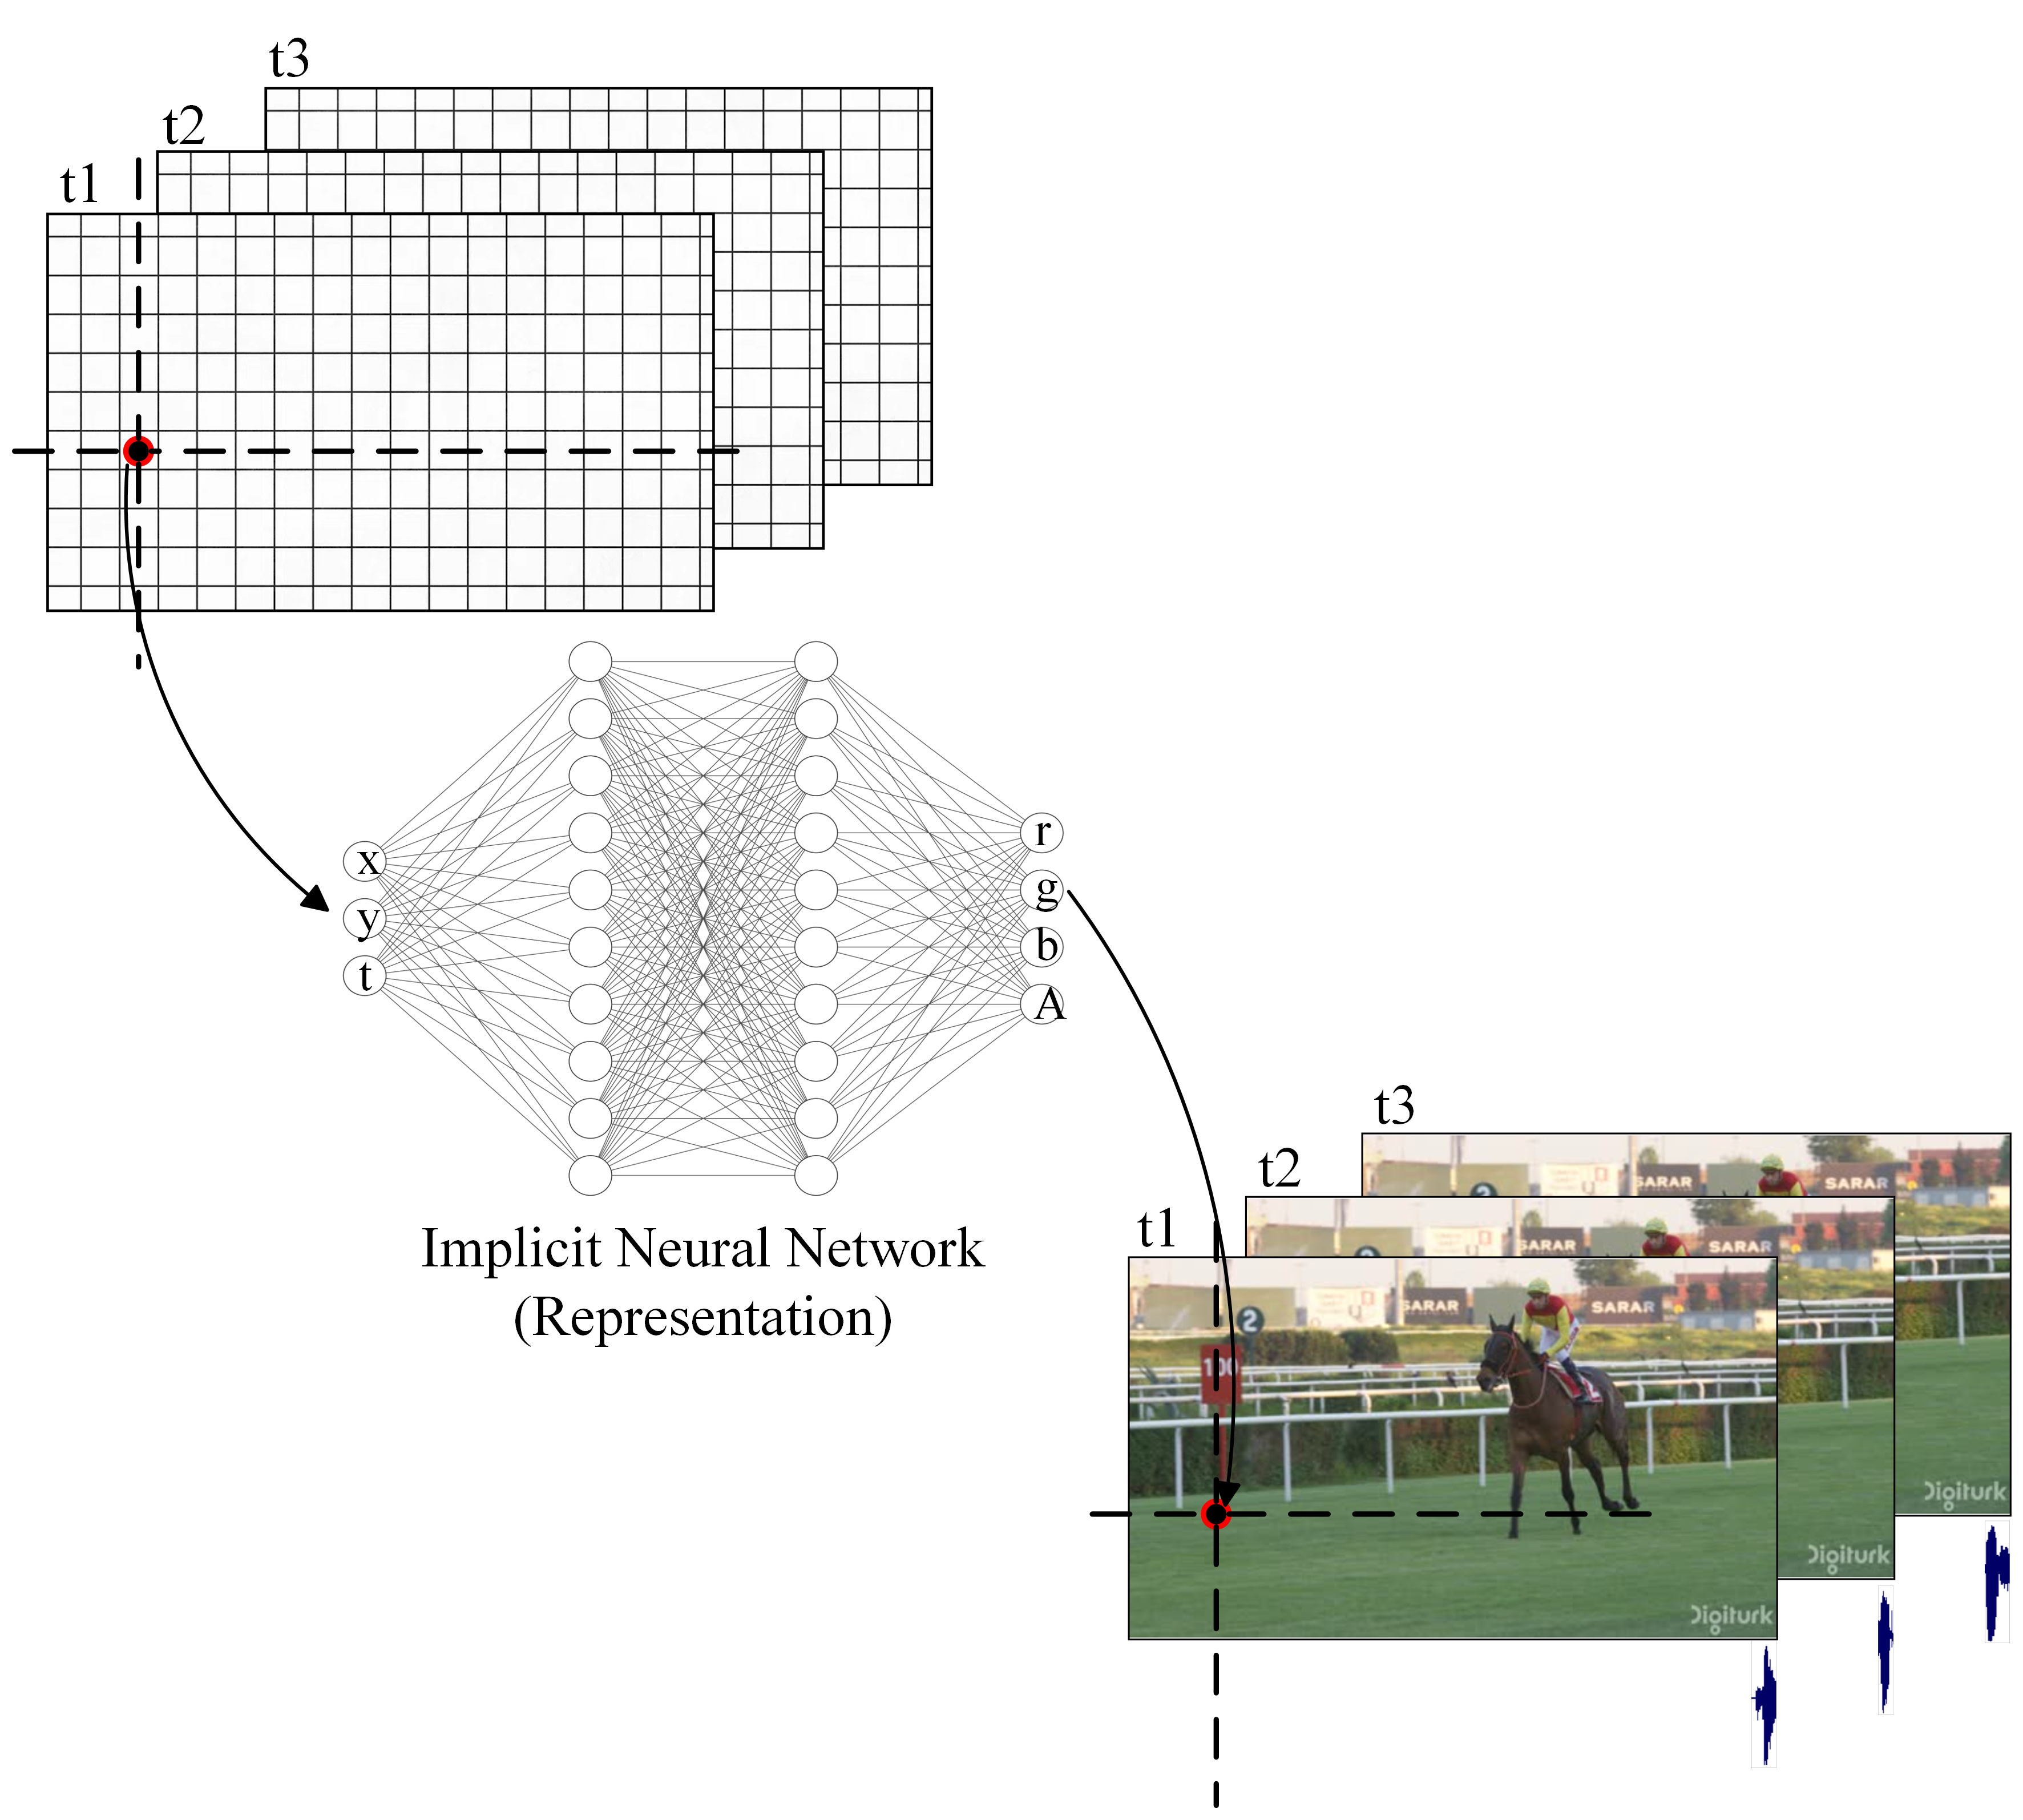
\includegraphics[height=0.45\textheight]{assets/INR.png}
        \caption{Representing Video in Neural Network}
        \label{fig:inr}
    \end{figure}
    \autoref{fig:inr} illustrates an Implicit Neural Representation (INR) where pixel coordinates $(x, y)$ and time index $t$ of video frames are fed into a neural network to output corresponding RGB values for visual data and amplitude for audio data. Sequential video frames $(t1, t2, t3)$ are divided into a grid of pixels. Each pixel's coordinates and time index are inputs to the network, which processes these inputs through several hidden layers. The network outputs the RGB values $(r, g, b)$ for each pixel's color and the amplitude $A$ for the associated audio. The outputs are then used to reconstruct the video frames and audio, demonstrating how the neural network encodes and decodes complex visual and audio information efficiently.
    \subsection{Fundamentals of INNs}
    \gls{inn} parameterize an unknown function \( f: \mathbb{R}^d \rightarrow \mathbb{R}^m \) where \( d \) and \( m \) represent the dimensions of the input and output spaces, respectively. This parameterization often involves a coordinate-based \gls{mlp} where the input coordinates are fed directly into the network, and the output is the function value at those coordinates. The network is trained using a loss function that minimizes the difference between the predicted and true function values over a set of sampled points.

    \subsection{Differences in Implicit Neural Network over Traditional Neural Network}

    The \autoref{fig:implicit-vs-traditional} provides a visual comparison between traditional neural networks and implicit neural networks like SIREN (Sinusoidal Representation Network). Traditional neural networks utilize a single set of shared weights and biases for all inputs, aiming to generalize across a dataset. This generalization allows the network to accurately classify or predict outcomes for new, unseen data based on its training. For instance, in the \autoref{fig:implicit-vs-traditional}, a traditional neural network trained on images of birds, reptiles, and mammals uses the same network architecture to classify any new image into these categories.

    In contrast, implicit neural networks represent each piece of media with its own unique neural network, characterized by distinct weights and biases. This approach fundamentally changes the way these networks operate. Overfitting, typically seen as a drawback in traditional neural networks, becomes a beneficial feature in implicit neural networks. Overfitting allows the network to memorize and accurately reproduce the intricate details and nuances of the specific piece of media it represents. For example, in the image, each silent video and audio clip has its own dedicated neural network that predicts frame-wise RGB values per pixel or time-wise amplitude values, respectively.

    The advantages of this approach are:

    \begin{itemize}
        \item \textbf{Detail Preservation:} The overfitting ensures that the network captures and reproduces fine-grained details of the media.
        \item \textbf{Per-Media Specialization:} Each piece of media is encoded into its unique network, allowing for highly specialized and optimized representations.
    \end{itemize}

    \begin{figure}[H]
        \centering
        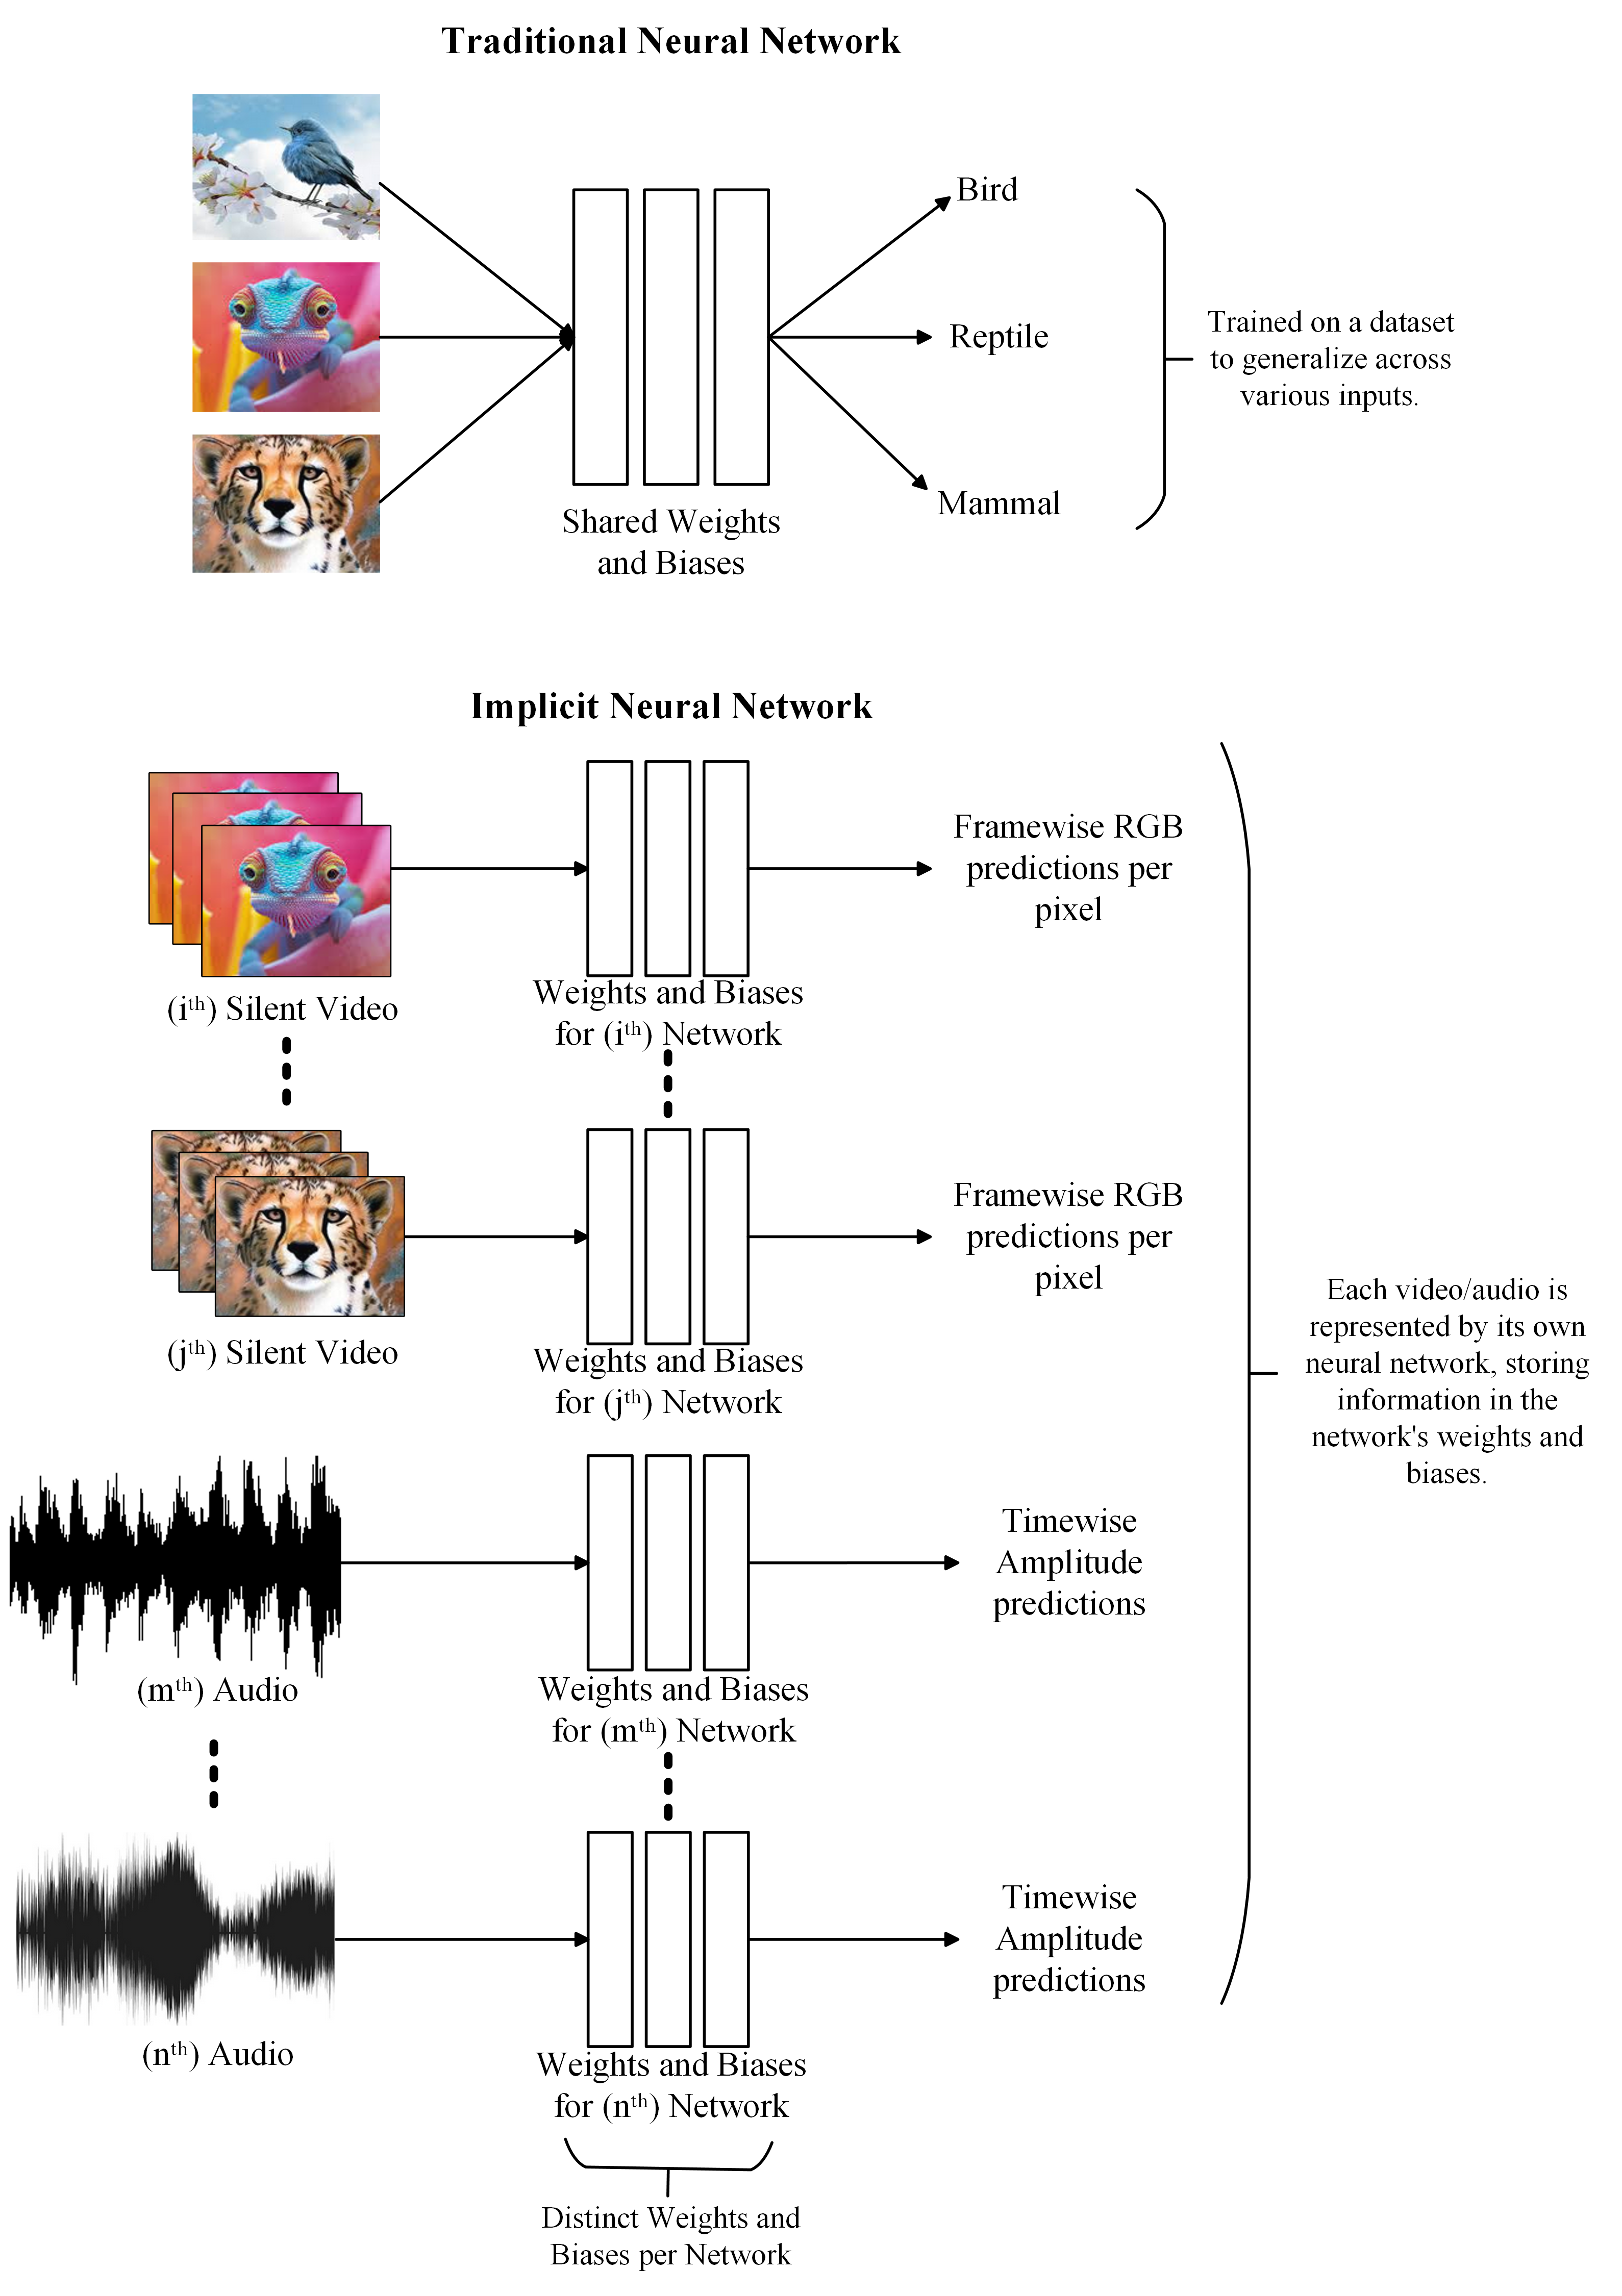
\includegraphics[width=0.95\linewidth]{assets/why overfitting.png}
        \caption{Implicit Neural Network vs Traditional Neural Network}
        \label{fig:implicit-vs-traditional}
    \end{figure}

    Thus implicit neural networks like \gls{siren} create unique networks for each media piece, leveraging overfitting to capture detailed representations. This allows implicit neural networks to store intricate details within their parameters, making overfitting a beneficial feature.
    
    
    \subsection{Significance of Sinusoidal Activations over Traditional Functions}

    The choice of activation functions in neural networks significantly influences their ability to model and process different types of data. The sine function is particularly suited for handling continuous inputs such as audio and video due to its inherent properties. Its smooth and periodic nature allows for efficient representation of continuous variations typical in audio waves or video frames. The smoothness of both the sine function and its derivative, a cosine wave, ensures that the gradients are well-defined across the entire function domain as shown in \autoref{fig:sinwave}. This characteristic is crucial during the neural network training process, which relies heavily on gradient-based optimization methods. The continuity and differentiability of the sine wave facilitate stable and effective weight updates, leading to reliable convergence in learning tasks.

    \begin{figure}[H]
        \centering
        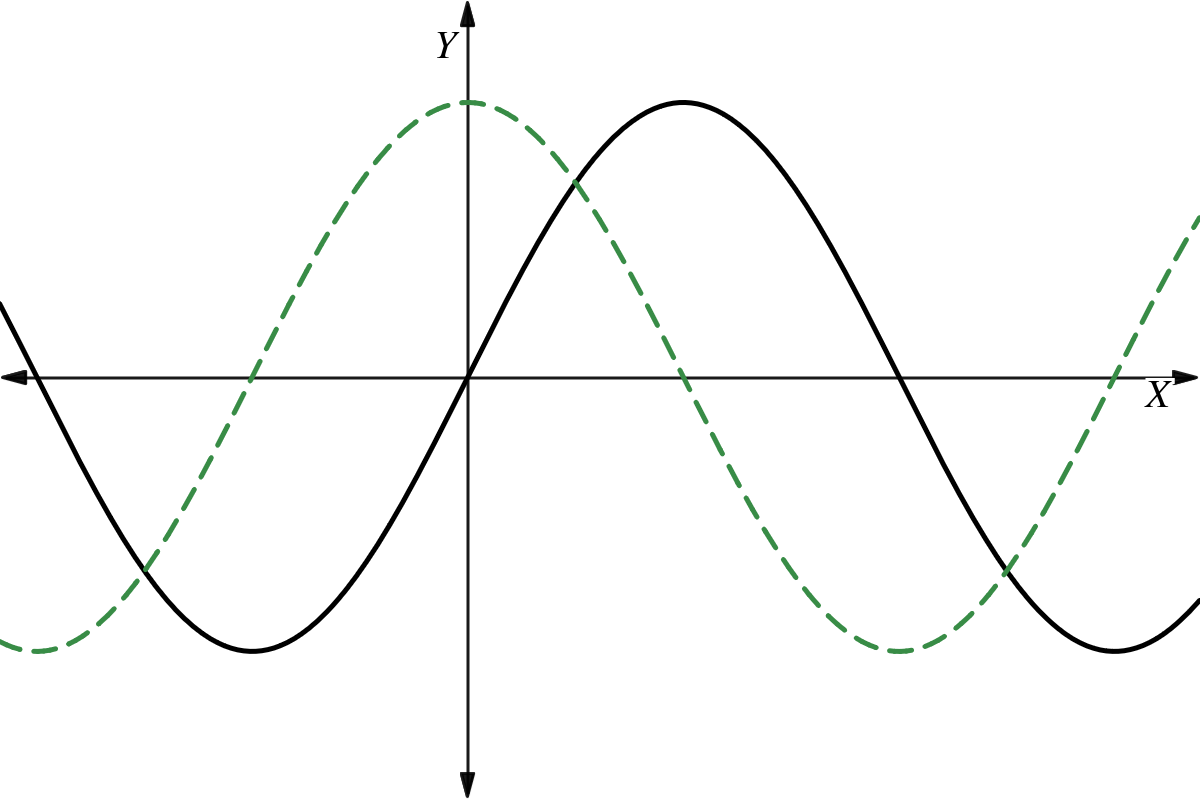
\includegraphics[height=0.25\textheight]{assets/sine-wave.png}
        \caption{Sine Wave and its Derivative}
        \label{fig:sinwave}
    \end{figure}

    In contrast, other waveforms like the triangular wave, although periodic, exhibit sharp transitions and corners at their peaks. The derivative of a triangular wave includes abrupt changes and discontinuities as we can see in \autoref{fig:triangular wave}, which can introduce complications in the learning process, particularly at points where the gradient becomes undefined. These discontinuities can potentially lead to instability in gradient calculations during backpropagation, adversely affecting the training efficiency and model performance. For neural networks involved in processing continuous data, such as in speech recognition or video processing, the sine function's ability to smoothly interpolate between values can capture complex, nuanced patterns more effectively. This smooth interpolation helps in better generalization and reduces the risk of overfitting to noisy variations, making the sine function a preferred choice for activation in networks dealing with continuous input signals.
    
    \begin{figure}[H]
        \centering
        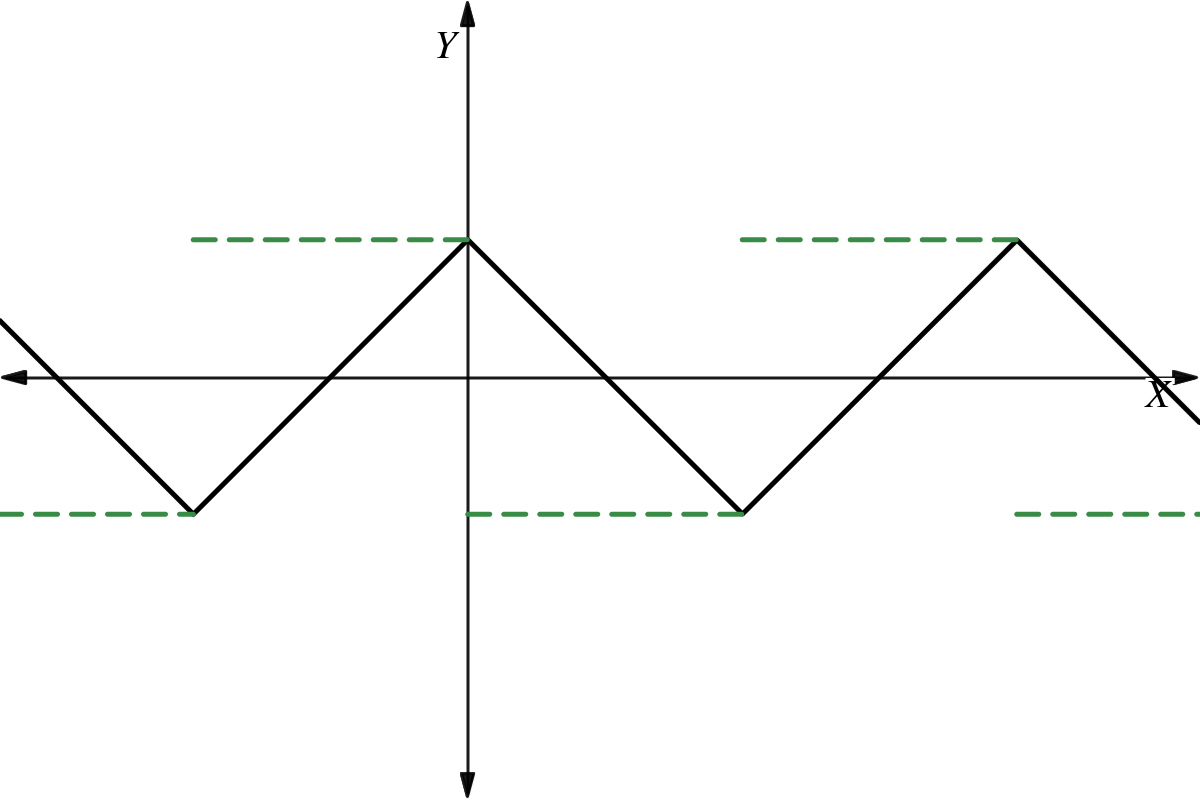
\includegraphics[height=0.25\textheight]{assets/triangular-wave.png}
        \caption{Triangular Wave and its Derivative}
        \label{fig:triangular wave}
    \end{figure}
    
    
    \begin{enumerate}[label=\textbf{\roman*.}]
        \item \textbf{Complex Signal Representation:} Sinusoidal activation functions enable neural networks to capture fine details and high-frequency components of signals more effectively. Traditional activation functions often struggle with this, leading to smoother, less detailed representations.
        \item \textbf{Smooth and Periodic Activation:} The smooth, continuous, and periodic nature of sinusoidal functions helps avoid issues like vanishing or exploding gradients, which are common with traditional activation functions, especially in deeper networks. This leads to more stable and efficient training dynamics.
        \item \textbf{Principled Initialization:} \gls{siren}s benefit from principled initialization scheme tailored for sinusoidal activations, ensuring that the network starts with a configuration that is conducive to learning complex patterns without the instability seen with other activation functions.
    \end{enumerate}
    
    \subsection{Transition to Sinusoidal Representation Networks (SIRENs)}
    Building on the concept of \gls{inn}, \gls{siren} introduce a critical innovation by employing sinusoidal activation functions in all layers of the network. The general form of a \gls{siren} layer is expressed as:
    \begin{equation}
        x_{i+1} = \sin(W_i x_i + b_i)
    \end{equation}
    
    where \( x_{i+1} \) is the output of the \(i\)-th layer, serving as the input to the next layer, \( \sin \) is the sinusoidal activation function applied to each layer, \( W_i \) is the weight matrix of the \(i\)-th layer, \( x_i \) is the input to the \(i\)-th layer, and \( b_i \) is the bias vector of the \(i\)-th layer.
    
    \subsection{Initialization Scheme for Sinusoidal Representation Networks (SIRENs)}
    Sinusoidal Representation Networks uses the sine function as an activation, which introduces sensitivity to input distributions due to its periodic nature. An effective initialization scheme is crucial to prevent the degradation of the network's performance with increasing depth. This report proposes a principled approach to initialization that preserves the distribution of activations across layers, ensuring that the output at initialization does not vary with the number of layers.
    \subsubsection{Steps Involved in Initialization}
    \begin{enumerate}[label=\textbf{\roman*.}]
        \item \textbf{Initial Input and Single Neuron Output}
        \begin{itemize}
            \item Uniformly Distributed Input: The input $x$ is drawn from a uniform distribution $U(-1, 1)$, representing normalized coordinates used in applications such as image processing.
            \item Output of a Single Sine Neuron: The output of a neuron using the sine activation function is given by:
               \begin{equation}
                  y = \sin(ax + b) 
               \end{equation} 
            where $a$ and $b$ are the frequency and phase parameters, respectively. For $a > \frac{\pi}{2}$, ensuring at least half a period of the sine function, the output distribution $y$ is arcsine distributed over $[-1, 1]$.
        \end{itemize}
        \item \textbf{Layer-wise Propagation}
        \begin{itemize}
            \item Weights and Biases: Weights $w$ are initialized uniformly within $U\left(-\frac{c}{\sqrt{n}}, \frac{c}{\sqrt{n}}\right)$ where, $c$ is a scaling factor and $n$ is the fan-in.
            \item Output of Deeper Layers: In subsequent layers, each input is arcsine distributed due to the previous layer's sine activation. The weighted sum $w^T x$ approaches a normal distribution as the number of inputs $n$ increases. Passing this sum through another sine function keeps the output arcsine distributed, preserving the distribution across layers.
        \end{itemize}
        \item \textbf{Special Handling in the First Layer} \\
          For the first layer, weights are adjusted by a factor $\omega_0$, set to 30. This adjustment ensures that the sine function: $\sin(\omega_0 \cdot Wx + b)$ spans multiple periods over the interval [-1, 1]. This extensive coverage is beneficial for handling the complex patterns and frequencies in video and audio data, enabling the network to capture a broad range of features initially.        
    \end{enumerate}


    \subsection{Siamese Siren}

    The Siamese Siren employs two neural networks with identical architectures but different weight initializations, referred to as the left and right Sirens. When an audio signal \( f \) is passed through these networks, they produce two slightly different outputs: \( f1 \) from the left Siren and \( f2 \) from the right Siren. These outputs, influenced by the slight variations in the networks, are then used to estimate and reduce noise.
    \begin{figure}[H]
        \centering
        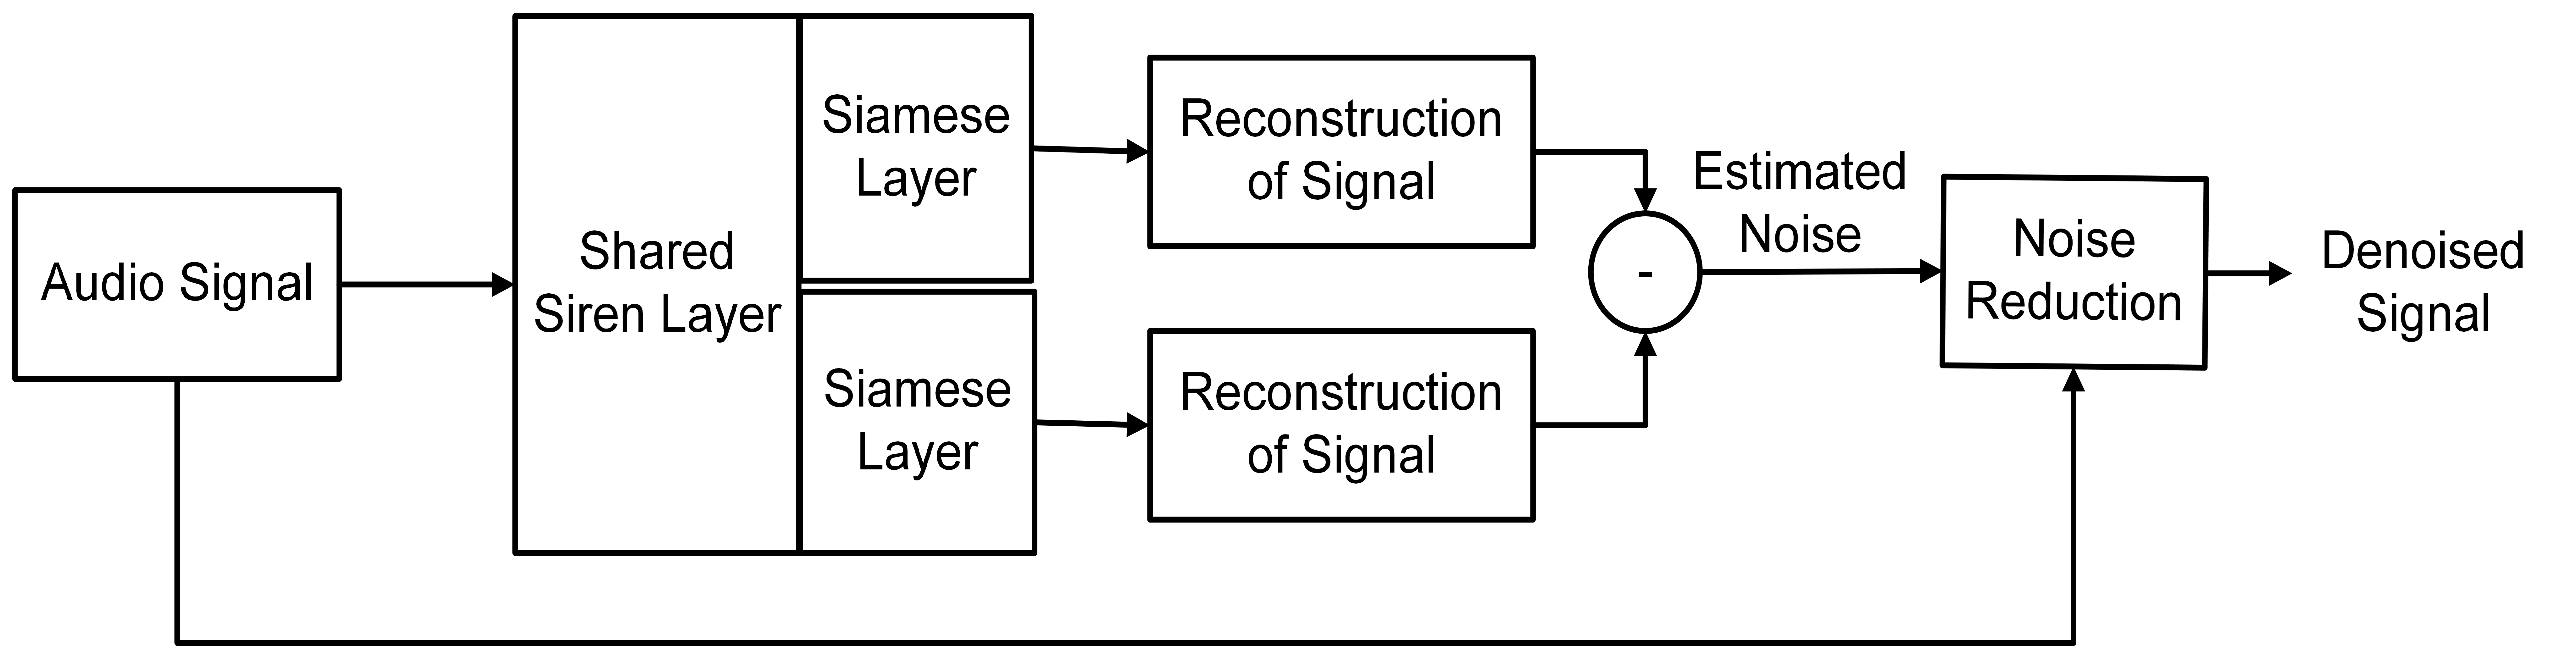
\includegraphics[width=\linewidth]{assets/Siamese_Siren_Block_Diagram.png}
        \caption{Siamese Siren Block Diagram}
        \label{fig:Siamese_Siren_Block_Diagram}
    \end{figure}

    \subsubsection{Noise Estimation in Siamese Siren}
    
    Siamese Siren estimates noise by calculating the difference between the outputs of the two networks:
    \begin{equation}
        \text{Noise} = f1 - f2
    \end{equation}
    where \( f1 \) is the inferenced audio from one network and \( f2 \) is the inferenced audio from the other network.
    
    \subsubsection{Noise Reduction Process}
    
    To reduce noise, the Siamese Siren leverages a noise reduction algorithm. This algorithm, often implemented using specialized noise reduction libraries, takes two inputs:
    \begin{enumerate}
        \item A noise estimation derived from the noisy audio.
        \item The noisy signal itself.
    \end{enumerate}

    \subsection{Knowledge Distillation for Model Compression}
    Knowledge distillation is a technique used in machine learning to transfer knowledge from a larger, more complex model (teacher) to a smaller, simpler model (student). This process aims to improve the efficiency and speed of the smaller model while maintaining or even enhancing its performance. One variant of knowledge distillation is \gls{rbkd}, which focuses on distilling knowledge related to the model's response or output behavior.

    The fundamental idea behind \gls{rbkd} is to train a student model to mimic not just the final predictions of the teacher model but also the intermediate responses or activations. This approach aims to capture the nuanced decision-making processes of the teacher model, enabling the student to generalize better and achieve comparable performance with fewer parameters.
    
    The main idea behind \gls{rbkd} revolves around the concept of feature representations and decision boundaries. By learning from the teacher model's response patterns, the student model can develop a deeper understanding of the underlying data distribution and make more informed predictions, especially in complex and high-dimensional input spaces.
    
    
    Soft Target Loss:
    The soft target loss remains the primary component in the distillation process. It compares the probabilities predicted by the student model to those of the teacher model:
    \begin{equation}
        L_{\text{soft}} = \frac{1}{N} \sum_{i=1}^{N} \left( S(x) - T(x)\right)^2
    \end{equation}
    
    where $L_{\text{soft}}$ is the soft target loss, $S(x)$ is the student model's output, and $T(x)$ is the teacher model's output for input $x$.

    Hard Target Loss:
    The hard target loss is an another component in response-based knowledge distillation. It compares the student model's predictions to the ground truth labels, ensuring that the student learns to represent the actual data accurately. The hard target loss is defined as:
    \begin{equation}
        L_{\text{hard}} = \frac{1}{N} \sum_{i=1}^{N} \left( S(x) - y\right)^2
    \end{equation}    
    
    where $L_{\text{hard}}$ is the soft target loss, $S(x)$ is the student model's output and $y$ is the ground truth label.

    The overall loss function simplifies to just the soft target loss without the response matching component:
    \begin{equation}
        L_{\text{total}} = \alpha L_{\text{soft}} + (1 - \alpha) L_{\text{hard}}
    \end{equation}

    where  $L_{\text{total}}$ is the total loss function, $\alpha$ is a hyperparameter controlling the importance of the soft target loss and hard target loss.
    
    In \autoref{fig:block-diagram-knowledge-distillation}, the teacher model is a SIREN (Sinusoidal Representation Networks) network pretrained on audio-visual data, while the student model is a shallower version designed to learn from the teacher's responses.
    
    The inputs to both models are in the form of (x, y, t), where (x, y) represent spatial coordinates in the video, and t represents time. The teacher model outputs four values: r, g, b (RGB values corresponding to (x, y, t)), and Amplitude (corresponding audio amplitude for the given (x, y, t)). Notably, the (x, y) coordinates are ignored in the context of audio amplitude.
    
    \begin{figure}[H]
        \centering
        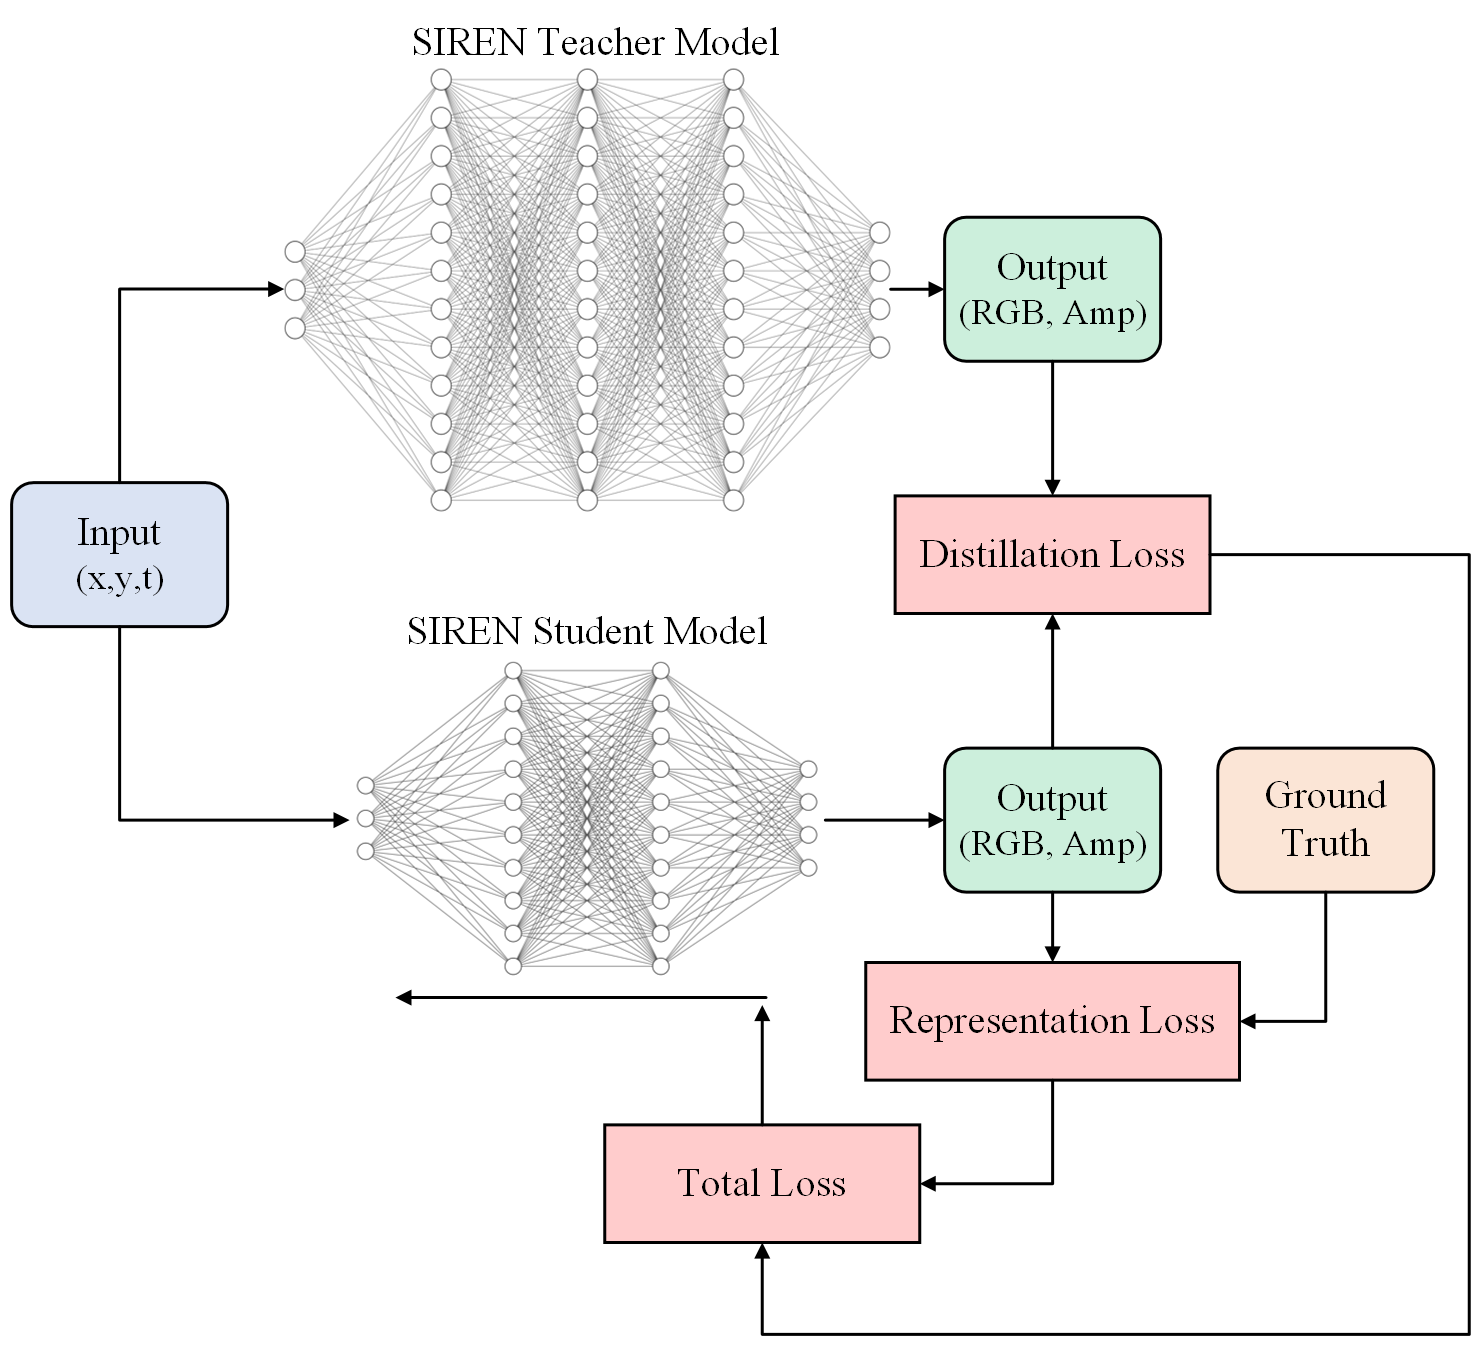
\includegraphics[width=0.95\linewidth]{assets/Knowledge Distillation.png}
        \caption{Block Diagram of Knowledge Distillation}
        \label{fig:block-diagram-knowledge-distillation}
    \end{figure}

    
    During response-based knowledge distillation, the student model's predictions are compared against the teacher model's predictions. This comparison helps calculate the distillation loss, which captures the discrepancy between the student's output and the teacher's output. Simultaneously, the ground truth provides the representation loss, measuring how well the student model represents the actual data.
    
    These two types of losses, distillation-loss and representation-loss, are weighted and combined to calculate the total loss. This total loss is then used for feedback and backpropagation during the training process, allowing the student model to gradually learn and mimic the behavior of the more complex teacher model.
    
    By using response-based knowledge distillation, the student model can benefit from the rich representations learned by the teacher model, even though it has a simpler architecture. This approach is particularly useful for tasks where computational resources or model complexity are constrained, yet high performance is desired.
      

    \subsection{Quantization}
    Quantization involves reducing the precision of the model's parameters, such as weights and biases, from floating-point to lower-bit representations, which decrease the model size.
    \begin{equation}
        w' = \text{round}\left(\frac{w}{s} + z \right)
    \end{equation}
    where, \( w \) is the original weight, \( s \) is a scaling factor, \( z \) is zero-point, and \( w' \) is the quantized weight.

    \begin{figure}[H]
            \centering
            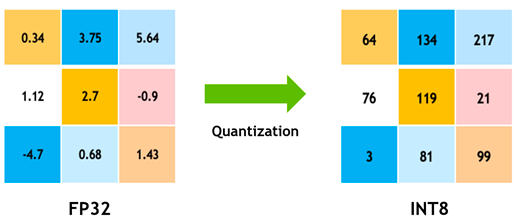
\includegraphics[width=\linewidth]{assets/quantization.png}
            \caption{Quantization}
            \label{fig:conceptual-quantization}
    \end{figure}
    In \autoref{fig:conceptual-quantization}, a sample 3x3 matrix of weights is taken. The weights are quantized to int 8, reducing the precision from 32-bit floating-point. This process reduces the model size and computational requirements, making it more efficient on resource-constrained devices.

    Since we will be using symmetric quantization for weights and biases of our model, we will discuss the symmetric quanzation below, however asymmetric quantization can also be done as shown in \autoref{app:quantization-manual-conversion}.
    \subsubsection{Symmetric Quantization} 
    \begin{figure}[H]
        \centering
        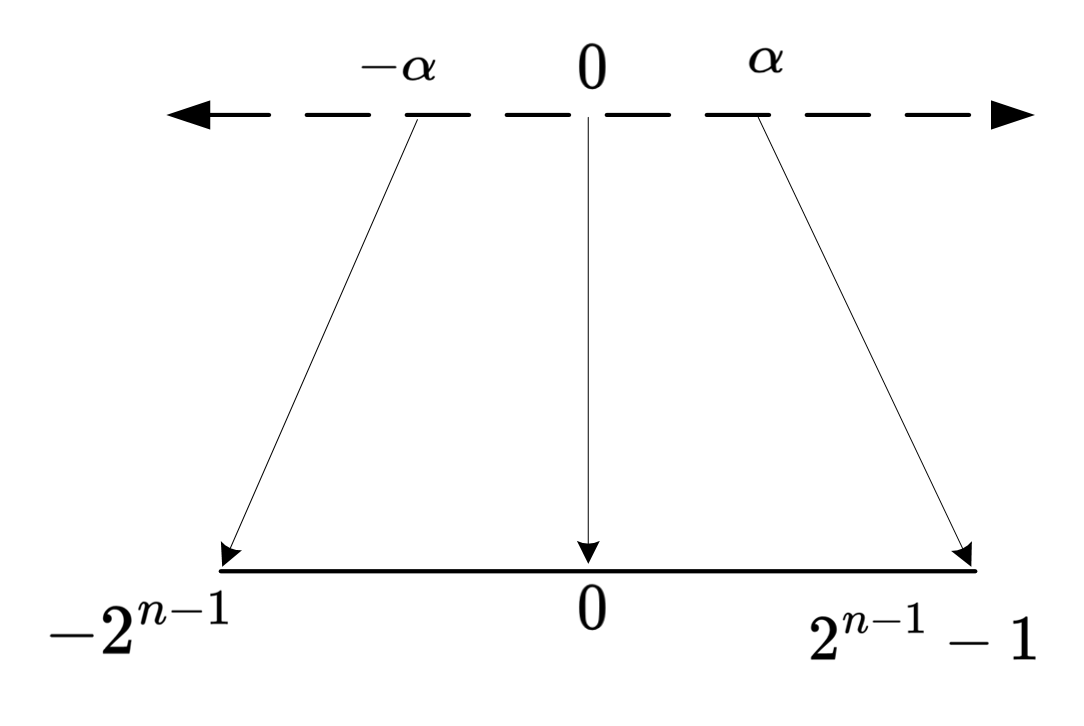
\includegraphics[width=0.7\linewidth]{assets/quantization/Symmetric_Qfigure.png}
        \caption{Symmetric Quantization}
        \label{fig:Symmetric_Qfigure}
    \end{figure}
    In symmetric quantization, the range of the values represented is symmetric around zero. This means the quantized values are distributed equally between positive and negative numbers.

    \textbf{Characteristics:}
    \begin{enumerate}
        \item Zero point is fixed at zero.
        \item Only scale factor is used to calculate quantized value.
    \end{enumerate}

    \subsection{Encoding}
    Encoding in the context of data compression refers to the process of converting raw data into a more compact representation, using techniques that minimize the amount of storage or transmission required. The goal of encoding is to reduce redundancy and increase efficiency, which can lead to significant reductions in the size of the data, making it easier to store and transfer.

    Two important methods for encoding data are Arithmetic Encoding and Range Encoding, which are widely used in various compression algorithms.

    \subsubsection{Aithmetic Encoding}
    Arithmetic Encoding is a form of entropy encoding that represents a message as a single number between 0 and 1. The key idea behind arithmetic encoding is to iteratively refine an interval to represent the entire message. Instead of encoding each symbol separately, arithmetic encoding encodes the entire message as a fraction in a range [0, 1].

    \begin{itemize}
        \item The process begins by initializing an interval [low, high], which initially spans the range [0, 1].
        \item For each symbol in the message, the interval is divided into subintervals based on the probabilities of the symbols. The interval is then updated based on the symbol's probability.
        \item The final encoded message is represented by a value within the resulting subinterval that corresponds to the entire message.
    \end{itemize}

    This method efficiently encodes data with different symbol frequencies and is highly effective in cases where symbols have different probabilities.

    \subsubsection{Range Encoding}

    \begin{figure}[H]
        \centering
        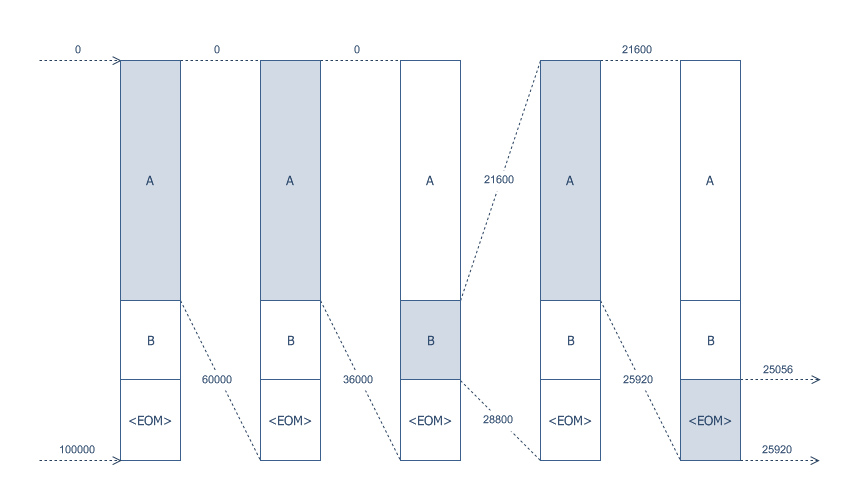
\includegraphics[width=0.95\linewidth]{assets/Range_encoding.jpg}
        \caption{Range Encoding}
        \label{fig:range_encoding}
    \end{figure}

    Range Encoding as shown in \autoref{fig:range_encoding} is similar to Arithmetic Encoding in that it also represents the entire message as a number within a range. However, Range Encoding uses a slightly different approach to dividing the range and updating it.

    \begin{itemize}
        \item Like arithmetic encoding, Range Encoding divides the range into subranges based on the probabilities of the symbols.
        \item However, Range Encoding works with fixed-size integers for each step, which makes it easier to implement and optimize.
        \item As each symbol is processed, the range is updated, and a final value within the range represents the compressed message.
    \end{itemize}

    While Range Encoding is simpler and faster than Arithmetic Encoding in practice, it can be less efficient when dealing with very large data sets or extremely small probabilities. Despite this, it remains popular in modern compression algorithms.

    \subsection{Compression Algorithms}
    Compression algorithms utilize encoding methods such as Arithmetic and Range Encoding to reduce the size of data. These algorithms are designed to identify patterns and redundancies in data, allowing them to replace these patterns with shorter representations, resulting in space savings.

    \subsubsection{LZMA Algorithm}
    The \gls{lzma} is a lossless data compression algorithm that employs both dictionary-based compression and range encoding. It is known for achieving very high compression ratios, making it a popular choice in formats such as 7z and xz.

    LZMA uses a hybrid approach by combining two key techniques:
    \begin{itemize}
        \item \textbf{Dictionary Compression:} \gls{lzma} maintains a sliding window (the dictionary), which stores previously seen data chunks. When encountering repeated sequences, \gls{lzma} replaces these sequences with references to their previous occurrences within the dictionary, allowing for significant compression.
        \item \textbf{Range Encoding:} To efficiently encode the references and symbols, \gls{lzma} uses Range Encoding. Range Encoding is applied to compress the frequency distribution of symbols and dictionary references. This step further reduces the size of the data by encoding the information in a compact form based on the likelihood of each symbol appearing.
    \end{itemize}

    The following is a simplified version of the \gls{lzma} algorithm:
    \begin{enumerate}[label=\textbf{\roman*.}]
        \item \textbf{Initialization:}
        \begin{itemize}
            \item Build a dictionary of size \texttt{window\_size} to store previously encountered data.
            \item Set up a range encoder to start encoding the output.
        \end{itemize}
        \item \textbf{Input Processing:}
        \begin{itemize}
            \item Read a chunk of data from the input stream.
            \item For each symbol, check if it exists in the dictionary.
            \item If the symbol exists, output a reference to the dictionary.
            \item If the symbol doesn't exist, output the symbol itself and add it to the dictionary.
        \end{itemize}
        \item \textbf{Range Encoding:}
        \begin{itemize}
            \item For each reference or symbol, use range encoding to map it to a smaller numerical range.
            \item Adjust the range based on the probability distribution of the symbols and references.
        \end{itemize}
        \item \textbf{Finalize:}
        \begin{itemize}
            \item Complete the encoding and output the final compressed data stream.
        \end{itemize}
    \end{enumerate}

    This hybrid approach makes \gls{lzma} both highly efficient and scalable, able to achieve impressive compression ratios even on large datasets.

    \subsubsection{xz}
    The xz compression format implements the \gls{lzma} algorithm, making use of the hybrid dictionary and range encoding approach to achieve high compression efficiency. xz is a popular compression utility used in Linux distributions and other environments that require strong compression performance.

    xz specifically implements \gls{lzma}2, a variant of the \gls{lzma} algorithm, which provides enhanced parallelism, allowing for better use of multi-core processors and increased compression speed without sacrificing compression ratio.

    Key characteristics of xz's implementation of \gls{lzma} are:

    \begin{itemize}
        \item \textbf{Dictionary Management:} Similar to \gls{lzma}, xz uses a dictionary-based approach where repeated strings in the input data are replaced by references to previous occurrences. This dictionary can be large and is critical for achieving high compression ratios.
        \item \textbf{Parallelization:} xz introduces the \gls{lzma}2 format, which divides the compression task into blocks. This allows multiple blocks to be compressed in parallel, making xz suitable for modern hardware with multiple processors or cores.
        \item \textbf{Range Encoding:} xz uses Range Encoding, just like \gls{lzma}, to encode the dictionary references and symbols, optimizing the final compressed output.
    \end{itemize}

    The xz format is widely used for distributing software packages, particularly in environments where high compression ratios are important. By implementing \gls{lzma}2 with range encoding and dictionary compression, xz can achieve impressive compression ratios while maintaining high performance.

    \subsection{MPEG Audio Layer 3}
    MPEG Audio Layer 3, commonly known as MP3, is a widely used audio compression standard that reduces file size while preserving perceptual audio quality. The encoding process involves several stages that progressively transform and compress the digital audio signal into a highly efficient format.
    
    \subsubsection{MPEG Audio Layer 3 Encoder}
        \begin{figure}[H]
            \centering
            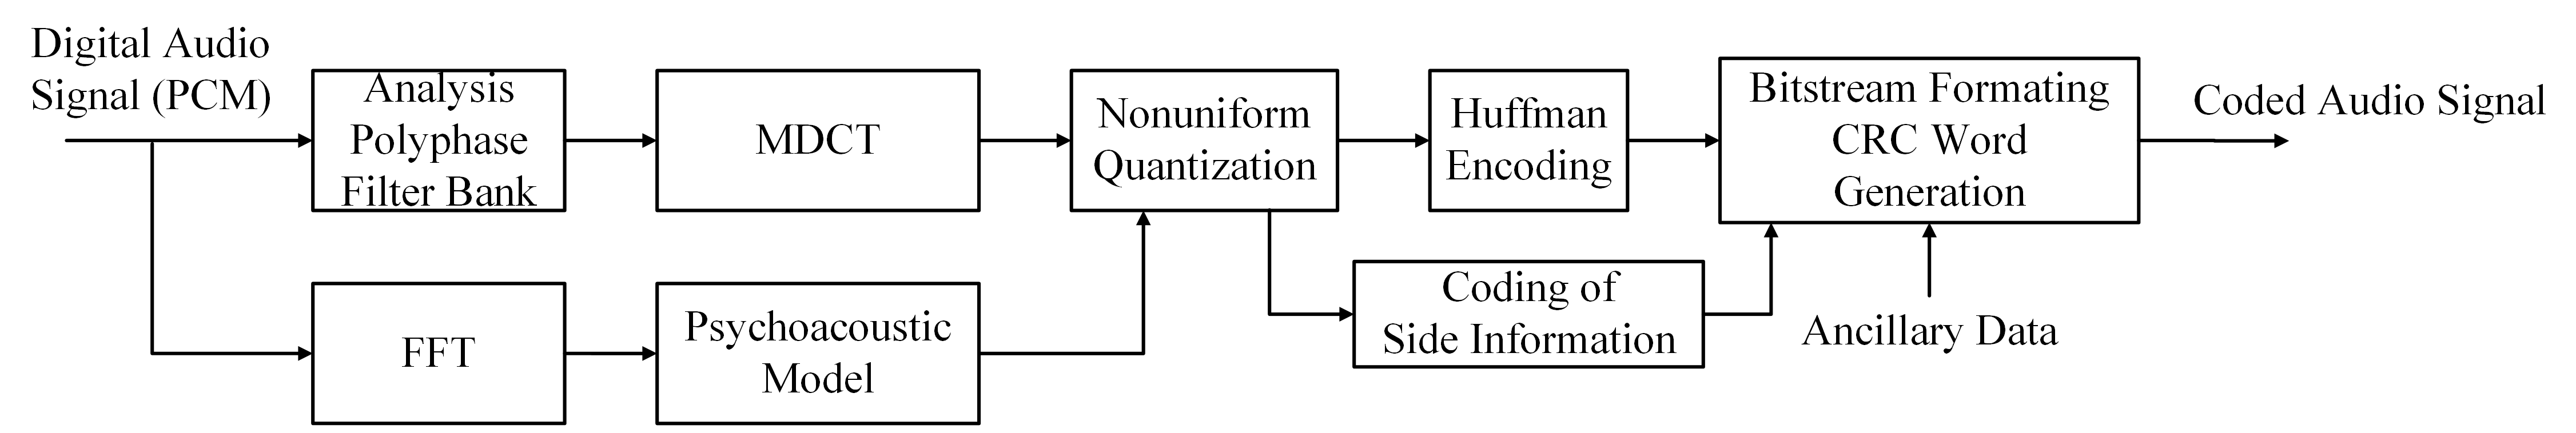
\includegraphics[width=0.95\linewidth]{assets/mp3_encoder.png}
            \caption{MPEG Audio Layer 3 Encoder}
            \label{fig:mp3_encoder}
        \end{figure}

        \begin{enumerate}[label=\textbf{\roman*.}]
            \item \textbf{Digital Audio Signal (PCM):}  
            \gls{pcm} represents the raw, uncompressed digital audio signal. It consists of sampled values of the original sound waveform, typically represented as 16-bit signed integers per sample. The input to the MP3 encoder is PCM audio, commonly sampled at rates like 44.1 kHz (CD quality) or 48 kHz.
        
            \item \textbf{Analysis Polyphase Filter Bank:}  
            This stage splits the audio signal into sub-bands or frequency bands using a polyphase filter bank. Dividing the signal into smaller frequency channels simplifies further processing and enables selective compression.
        
            \item \textbf{FFT (Fast Fourier Transform):}  
            The \gls{fft} converts the time-domain audio signal into the frequency domain. This transformation identifies the energy in different frequency components (sine waves) of the audio, providing insight into the spectral content.
        
            \item \textbf{Psychoacoustic Model:}  
            The psychoacoustic model applies principles of human hearing to discard inaudible data.
            \begin{itemize}
                \item Frequencies above 20 kHz or below the threshold of hearing are removed.
                \item Masking effects eliminate inaudible sounds masked by louder frequencies.
                \item Loudness analysis determines the importance of each frequency band, prioritizing perceptually significant data.
            \end{itemize}
        
            \item \textbf{MDCT (Modified Discrete Cosine Transform):}  
            \gls{mdct} further processes the frequency data by converting overlapping audio blocks into the frequency domain. It reduces blocking artifacts and provides better time-frequency resolution. This step ensures accurate reconstruction during decoding.
        
            \item \textbf{Nonuniform Quantization:}  
            The MDCT coefficients are quantized to compress the audio further:
            \begin{itemize}
                \item Frequencies less perceptible to the human ear are quantized with less precision.
                \item This step introduces bit-rate control, selectively reducing precision to minimize file size while maintaining quality.
            \end{itemize}
        
            \item \textbf{Huffman Encoding:}  
            A lossless compression technique is applied to the quantized data. Huffman encoding assigns shorter codes to frequently occurring values, optimizing the overall file size.
        
            \item \textbf{Bitstream Formatting and CRC Word Generation:}  
            The encoded audio data is organized into a structured bitstream. \gls{crc} data is added to verify data integrity during transmission.
        
            \item \textbf{Coding of Side Information:}  
            Side information includes metadata required for decoding:
            \begin{itemize}
                \item Sampling rate
                \item Bitrate
                \item Frame length
                \item Quantization details
            \end{itemize}
            This ensures accurate reconstruction of the audio.
        
            \item \textbf{Ancillary Data:}  
            Optional ancillary data, such as metadata (ID3 tags), album art, or custom data, can be embedded in the MP3 file. Although not required for decoding, it adds extended functionality.
        \end{enumerate}

        \subsubsection{MPEG Audio Layer 3 Decoder}

        \begin{figure}[H]
            \centering
            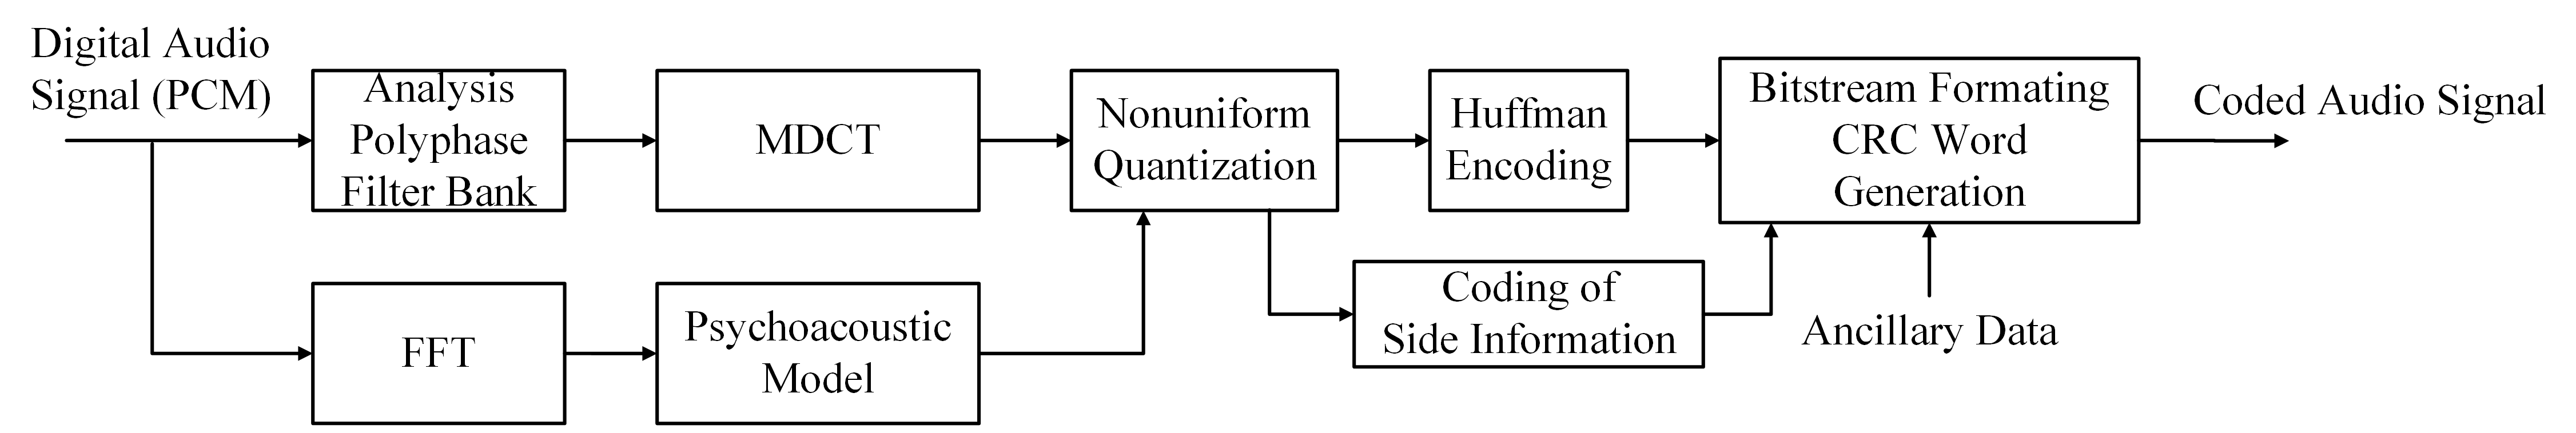
\includegraphics[width=0.95\linewidth]{assets/mp3_encoder.png}
            \caption{MPEG Audio Layer 3 Decoder}
            \label{fig:mp3_decoder}
        \end{figure}
        
        \begin{enumerate}[label=\textbf{\roman*.}]
            \item \textbf{Bitstream:}  
            The bitstream is the compressed MP3 file produced during encoding. It contains the encoded audio data along with side information necessary for decoding.
        
            \item \textbf{Synchronization and Error Checking:}  
            This block resolves synchronization issues in the bitstream and verifies its integrity using techniques like CRC (Cyclic Redundancy Check).
        
            \item \textbf{Huffman Decoding:}  
            This step reverses the Huffman encoding applied during compression, recovering the quantized audio data.
        
            \item \textbf{Scalefactor Decoding:}  
            The scalefactor values embedded in the bitstream are decoded. These values are crucial for restoring the magnitude of the frequency-domain coefficients.
        
            \item \textbf{Descaling:}  
            The quantized values are rescaled to their proper range to ensure accurate reconstruction of the audio data.
        
            \item \textbf{Reordering:}  
            The data reordered during encoding for compression efficiency is restored to its original order.
        
            \item \textbf{Joint Stereo Decoding:}  
            If joint stereo techniques were used in encoding, the stereo channels are reconstructed. This step restores the correlation between the left and right channels.
        
            \item \textbf{Alias Reduction:}  
            Alias reduction eliminates aliasing artifacts caused during the encoding process, ensuring clean audio output.
        
            \item \textbf{IMDCT (Inverse Modified Discrete Cosine Transform):}  
            The \gls{imdct} step reverses the \gls{mdct} transformation applied during encoding, converting frequency-domain data back into the time domain.
        
            \item \textbf{Frequency Inversion:}  
            Any frequency inversion applied during encoding is reversed in this step.
        
            \item \textbf{Synthesis Polyphase Filter Bank:}  
            The Synthesis Polyphase Filter Bank reconstructs the original time-domain signal from the time-frequency data. It operates as the inverse of the Analysis Polyphase Filter Bank used during encoding.
        
            \item \textbf{PCM Output:}  
            The final output is in Pulse Code Modulation \gls{pcm} format, an uncompressed audio representation ready for playback. Separate left and right channels are produced for stereo audio.
        \end{enumerate}
        
    \subsection{Advanced Video Codec (AVC) }
        \begin{figure}[H]
        \centering
        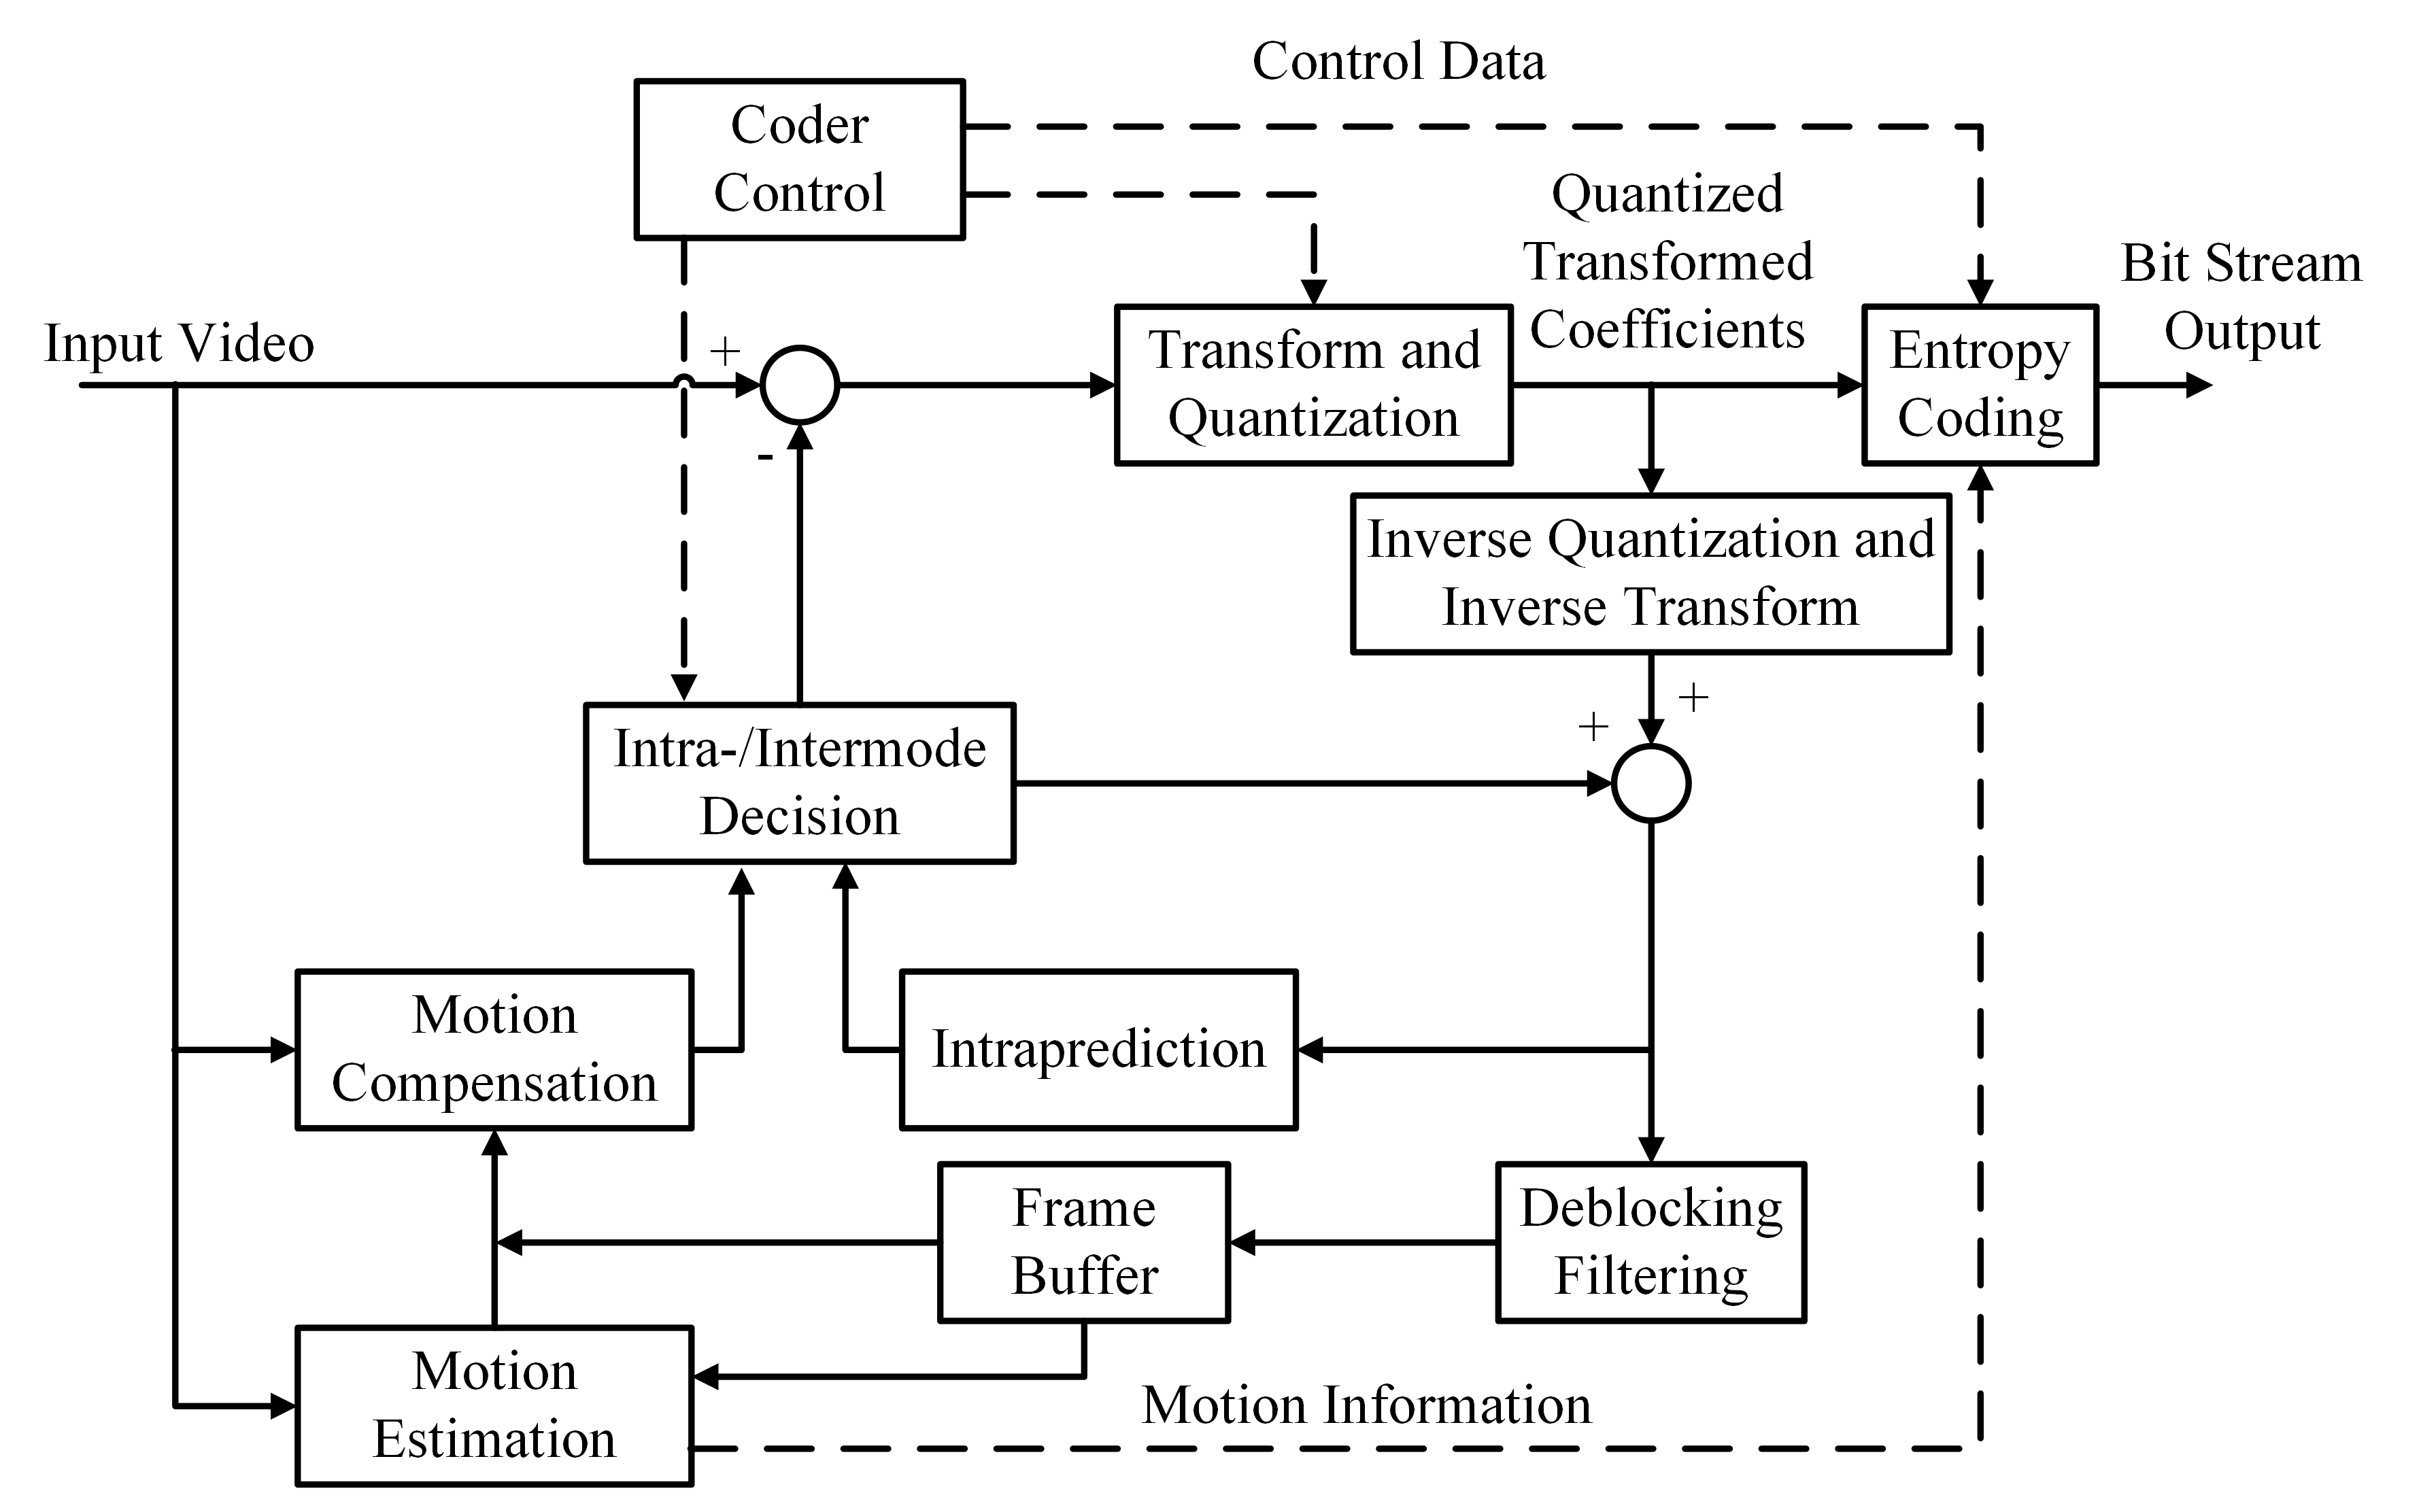
\includegraphics[width=0.95\linewidth]{assets/h264_blockdiagram.png}
        \caption{Block Diagram of Advanced Video Codec}
        \label{fig:avc}
    \end{figure}

    \autoref{fig:avc} outlines the encoding process for the Advanced Video Codec. The process involves a series of steps, starting with the input video and proceeding through various prediction, transformation, and compression techniques to produce a highly efficient encoded bitstream. 

    \begin{enumerate}[label=\textbf{\roman*.}]
        \item \textbf{Input Video:}  
        The process begins with an input video consisting of a sequence of frames, each composed of three components: luminance (Y) and chrominance (Cb and Cr). The luminance provides brightness information, while chrominance adds color details. Frames are divided into macroblocks of $16 \times 16$ pixels for Y and $8 \times 8$ pixels for Cb and Cr.
    
        \item \textbf{Intra-/Intermode Decision:}  
        This step determines how each macroblock will be encoded.
        \begin{itemize}
            \item \textbf{Intra-mode:} Macroblocks are predicted based on previously encoded blocks within the same frame. This mode is effective for spatial redundancy.
            \item \textbf{Inter-mode:} Macroblocks are predicted using reference frames from the past or future. This mode is effective for temporal redundancy.
        \end{itemize}
    
        \item \textbf{Motion Estimation:}  
        When inter-mode is selected, motion estimation determines object movement relative to reference frames.
        \begin{itemize}
            \item Macroblocks can be divided into smaller partitions (e.g., $16 \times 16$, $8 \times 8$, $4 \times 4$).
            \item Motion vectors with sub-pixel precision (e.g., quarter-pixel for luma) are calculated.
            \item A search algorithm minimizes differences between current and reference macroblocks.
        \end{itemize}
    
        \item \textbf{Motion Compensation:}  
        Using motion vectors, motion compensation reconstructs predicted macroblocks.
        \begin{itemize}
            \item Fractional-pixel values are interpolated using filters like six-tap FIR filters.
            \item Multiple reference frames enhance prediction accuracy.
        \end{itemize}
    
        \item \textbf{Intraprediction:}  
        When intra-mode is selected, predictions rely on spatial redundancy:
        \begin{itemize}
            \item Macroblocks are predicted using neighboring reconstructed macroblocks.
            \item Prediction modes include:
            \begin{itemize}
                \item $4 \times 4$ blocks: Nine directional modes.
                \item $8 \times 8$ blocks: Nine modes.
                \item $16 \times 16$ macroblocks: Four modes.
            \end{itemize}
        \end{itemize}
    
        \item \textbf{Residual Calculation:}  
        The residual is calculated by subtracting the predicted macroblock from the actual macroblock, representing the difference or error for compression.
    
        \item \textbf{Transform and Quantization:}  
        \textit{Transformation:} Converts residuals into the frequency domain using an integer transform derived from the \gls{dct}, reducing spatial redundancy. \\
        \textit{Quantization:} Reduces the precision of transformed coefficients:
        \begin{itemize}
            \item Low-frequency components are preserved for quality.
            \item High-frequency components are aggressively compressed.
        \end{itemize}
    
        \item \textbf{Entropy Coding:}  
        Encodes quantized coefficients, motion vectors, and control data into a compressed bitstream.
        \begin{itemize}
            \item \textbf{CAVLC:} Context-Adaptive Variable Length Coding.
            \item \textbf{CABAC:} Context-Adaptive Binary Arithmetic Coding.
        \end{itemize}
    
        \item \textbf{Deblocking Filtering:}  
        Mitigates blocking artifacts introduced by quantization.
        \begin{itemize}
            \item Adaptive filtering smooths block boundaries.
            \item Strength is adjusted based on slice, block edge, and pixel levels.
        \end{itemize}
    
        \item \textbf{Inverse Transform and Inverse Quantization:}  
        Quantized coefficients are inverse-quantized and transformed back to the spatial domain. Reconstructed residuals are added to predictions to recreate macroblocks.
    
        \item \textbf{Frame Buffer:}  
        Stores reference frames.
        \begin{itemize}
            \item Short-term frames for recent predictions.
            \item Long-term frames for scalability and large temporal gaps.
        \end{itemize}
    
        \item \textbf{Output Bit Stream:}  
        Produces a final encoded bitstream containing motion vectors, quantized residual coefficients, prediction modes, and control information.
    \end{enumerate}

    \subsection{High Efficiency Video Coding (HEVC)}
        \begin{figure}[H]
        \centering
        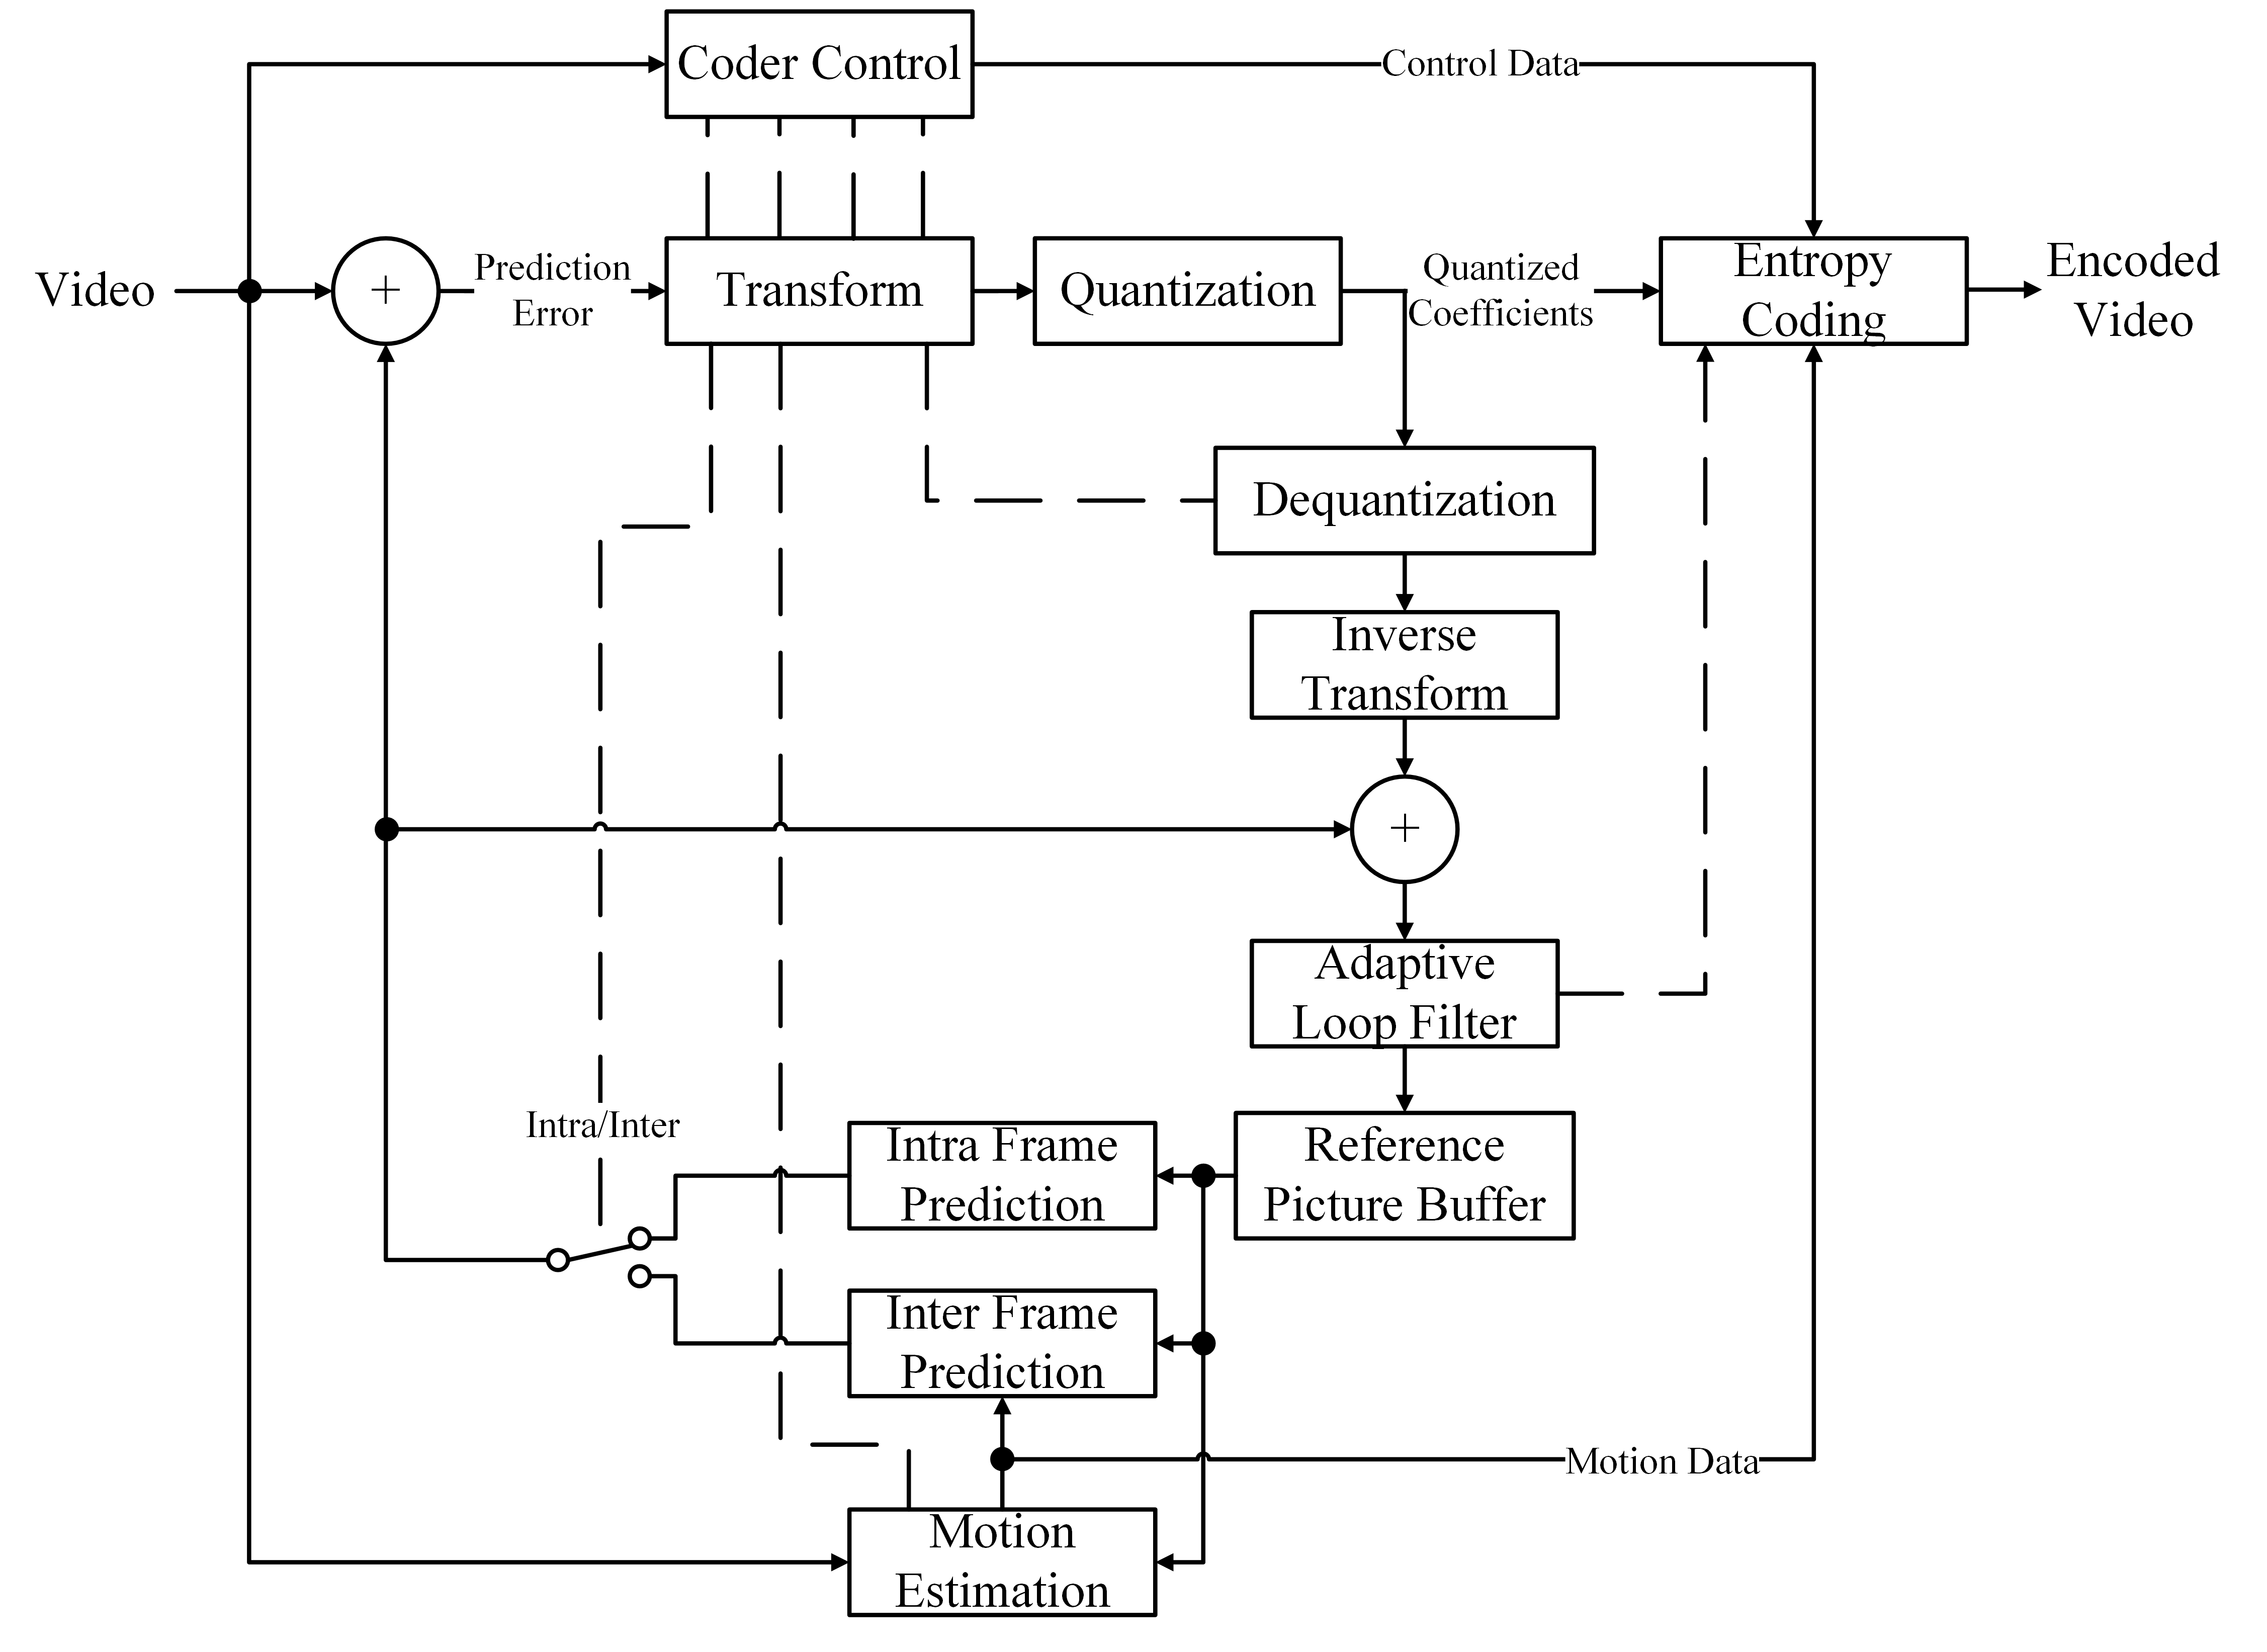
\includegraphics[width=0.95\linewidth]{assets/h265_blockdiagram.png}
        \caption{Block Diagram of High Efficiency Video Coding}
        \label{fig:hevc}
    \end{figure}

    The block diagram of \gls{hevc} shares a similar high-level structure with \gls{avc}, reflecting its hybrid coding framework based on intra-frame and inter-frame prediction, transform, quantization, and entropy coding. However, \gls{hevc} introduces several key advancements to improve compression efficiency, particularly for high-resolution content. Additionally, some blocks in \gls{hevc} feature entirely new functionalities.

    \begin{enumerate}[label=\textbf{\roman*.}]
        \item \textbf{Input Video:}  
        \gls{hevc} processes input video frames divided into luminance (Y) and chrominance (Cb, Cr) components, similar to H.264. However, HEVC replaces macroblocks with flexible Coding Tree Units (CTUs), which can be as large as 64×64 and recursively partitioned into smaller Coding Units (CUs), down to 8×8. This flexibility reduces overhead for high-resolution content.
    
        \item \textbf{Intra-/Intermode Decision:}  
        \gls{hevc} decides between intra-prediction (within a frame) and inter-prediction (between frames) based on the redundancy present. It offers 35 intra-prediction modes for luma and 6 for chroma, significantly improving texture handling compared to H.264's limited modes. Inter-prediction is enhanced with asymmetric motion partitions (AMPs) and motion merge mode.
    
        \item \textbf{Motion Estimation and Compensation:}  
        \gls{hevc} uses refined sub-pixel precision for motion estimation, improving upon H.264's quarter-pixel accuracy. Sophisticated search strategies optimize motion vectors and reduce complexity. Motion merge mode reuses parameters to compress the bitstream further, while multi-reference frame compensation improves prediction accuracy.
    
        \item \textbf{Transform and Quantization:}  
        \gls{hevc} supports larger transform block sizes (up to 32×32) compared to H.264's maximum of 8×8, enhancing compression for smooth areas. It introduces the Discrete Sine Transform (DST) for intra-predicted blocks and uses improved quantization techniques, simplifying the decoding process.
    
        \item \textbf{Entropy Coding:}  
        \gls{hevc} exclusively employs Context-Adaptive Binary Arithmetic Coding (CABAC), optimizing it for larger block sizes and parallel processing, unlike H.264, which also used the less efficient Context-Adaptive Variable Length Coding (CAVLC).
    
        \item \textbf{Deblocking Filter:}  
        \gls{hevc} improves deblocking decisions by considering multiple block boundary types (e.g., CUs, PUs, TUs). This provides better artifact suppression, especially for high-resolution content.
    
        \item \textbf{Adaptive Loop Filtering (ALF):}  
        \gls{hevc} applies adaptive filters optimized for each frame's content, reducing distortions introduced during encoding. This ensures better visual quality by minimizing blocking and blurring artifacts.
    
        \item \textbf{Reference Picture Buffer:}  
        \gls{hevc} stores reference frames in an optimized buffer, supporting larger coding tree units and parallel processing methods like wavefront parallel processing.
    
        \item \textbf{Coder Control:}  
        \gls{hevc} integrates advanced coder control to manage partitioning, mode selection, and bit allocation. It supports parallel encoding strategies to maximize multi-core processor efficiency.
    \end{enumerate}


\pagebreak


\section{\MakeUppercase{Mathematical Formulation}}

\subsection{Mathematical Modeling in SIRENs}
\gls{siren} excel in tasks requiring the modeling of periodic and smooth phenomena, which are common in audio and video signals. The continuous nature of the function modeled by \gls{siren} makes them ideal for compressing these signals efficiently. The typical loss function used for training \gls{siren} in the context of compression is the \gls{mse}, which ensures the fidelity of the reconstructed signal:
\begin{equation}
    L = \frac{1}{N} \sum_{n=1}^N (\Phi(\mathbf{x}_n) - y_n)^2 
\end{equation}
Additionally, to capture temporal dynamics in video and audio, derivatives of the function are often included in the training objective:
\begin{equation}
    L = \frac{1}{N} \sum_{n=1}^N \left((\Phi(\mathbf{x}_n) - y_n)^2 + \lambda (\nabla\Phi(\mathbf{x}_n) - \nabla y_n)^2\right) 
\end{equation}
where, \( N \) is the total number of sampled points, \( \Phi \) is the SIREN model, \( \mathbf{x}_n \) are the input coordinates for the \(n\)-th data point, \( y_n \) are the actual output values at the \(n\)-th data point, \( \lambda \) is a regularization parameter, \( \nabla\Phi(\mathbf{x}_n) \) is the derivative of the \gls{siren} output with respect to the input at \( \mathbf{x}_n \), and \( \nabla y_n \) is the derivative of the true output values with respect to the input at \( \mathbf{x}_n \).


\subsection{Forward and Backward Propagation in SIREN Network}
\begin{figure}[H]
    \centering
    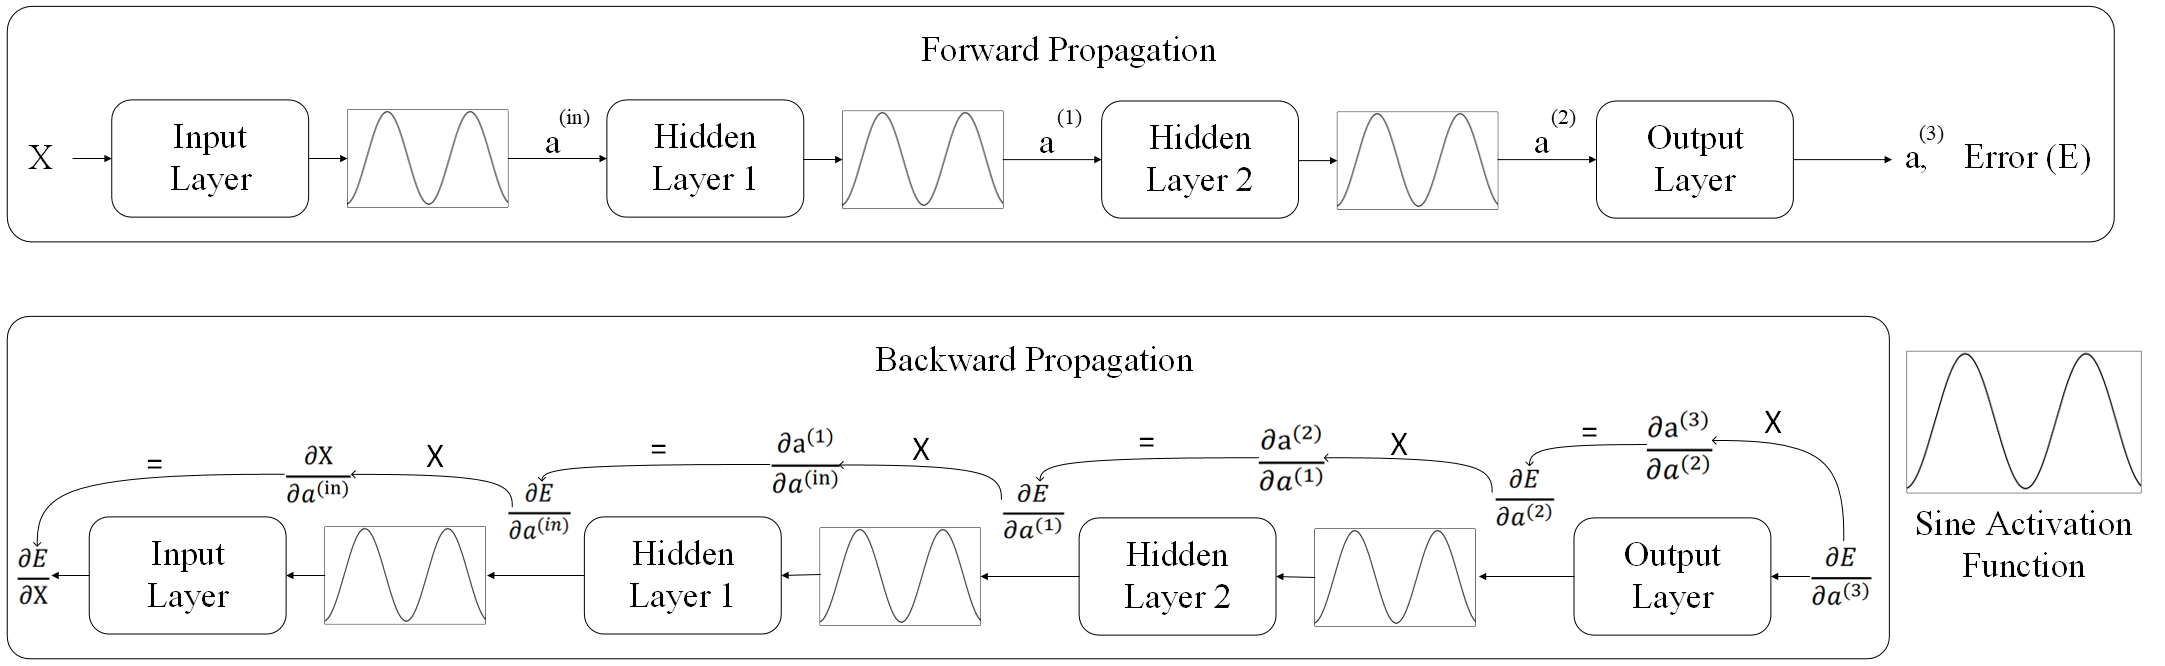
\includegraphics[width=\linewidth]{assets/Propagation concept figure Major Project.png}
    \caption{Forward and Backward Propagation in SIREN Network}
    \label{fig:propagation-diagram}
\end{figure}

The figure provides an illustration of the forward and backward propagation processes in a \gls{siren} neural network. In the forward propagation section, the input \( \mathbf{X} \) is passed through the input layer, then sine activation is applied, and then sequentially through hidden layers 1 (with sine activation) and hidden layer 2 (with sine activation), and finally through the output layer. The forward propagation process can be described by the equations:
\begin{equation}
    \mathbf{Z}^{(l)} = \mathbf{W}^{(l)T} \mathbf{a}^{(l-1)} + \mathbf{b}^{(l)}
\end{equation}
\begin{equation}
    \mathbf{a}^{(l)} = \sin(\mathbf{Z}^{(l)})
\end{equation}
where,
\begin{itemize}
    \item \( \mathbf{Z}^{(l)} \) is the linear combination of inputs at layer \( l \).
    \item \( \mathbf{W}^{(l)} \) represents the weights of the \( l \)-th layer.
    \item \( \mathbf{a}^{(l-1)} \) is the activation from the previous layer.
    \item \( \mathbf{b}^{(l)} \) represents the biases of the \( l \)-th layer.
    \item \( \mathbf{a}^{(l)} \) is the activation of the \( l \)-th layer after applying the sine function.
\end{itemize}

The error \( \mathbf{E} \) is calculated based on the difference between the predicted output \( \mathbf{a}^{(3)} \) and the actual output \( \mathbf{y}_i \). Specifically, we use the Mean Squared Error (MSE) loss function:
\begin{equation}
    \mathbf{E} = \frac{1}{2} \sum_{i=1}^{N} (\mathbf{a}^{(3)}_i - \mathbf{y}_i)^2
\end{equation}
where,
\begin{itemize}
    \item \( \mathbf{a}^{(3)}_i \) is the predicted output.
    \item \( \mathbf{y}_i \) is the actual output.
\end{itemize}

The backward propagation section shows the gradient calculation needed to update the network's weights. It starts with the error gradient \( \frac{\partial \mathbf{E}}{\partial \mathbf{a}^{(3)}} \) at the output layer and propagates backwards through hidden layers 2 and 1, and finally to the input layer. This involves computing the gradients \( \frac{\partial \mathbf{a}^{(3)}}{\partial \mathbf{a}^{(2)}} \), \( \frac{\partial \mathbf{a}^{(2)}}{\partial \mathbf{a}^{(1)}} \), and \( \frac{\partial \mathbf{a}^{(1)}}{\partial \mathbf{a}_{(in)}} \).

The weights and biases are updated as per the following equations:
\begin{equation}
    \mathbf{W}^{(l)} \leftarrow \mathbf{W}^{(l)} - \eta \frac{\partial \mathbf{E}}{\partial \mathbf{W}^{(l)}}  
\end{equation}
\begin{equation}
    \mathbf{b}^{(l)} \leftarrow \mathbf{b}^{(l)} - \eta \frac{\partial \mathbf{E}}{\partial \mathbf{b}^{(l)}}  
\end{equation}

where,
\begin{itemize}
    \item \( \mathbf{W}^{(l)} \) represents the weights of the \( l \)-th layer.
    \item \( \mathbf{b}^{(l)} \) represents the biases of the \( l \)-th layer.
    \item \( \eta \) is the learning rate.
    \item \( \frac{\partial \mathbf{E}}{\partial \mathbf{W}^{(l)}} \) is the gradient of the error with respect to the weights of the \( l \)-th layer.
    \item \( \frac{\partial \mathbf{E}}{\partial \mathbf{b}^{(l)}} \) is the gradient of the error with respect to the biases of the \( l \)-th layer.
\end{itemize}

The detailed forward and backward propagation equations and the gradients of error with respect to weight and bias matrices are provided in \autoref{app:forward-backward-eqn}.


\subsection{Quantization Modeling}
Quantization maps a floating-point weight \( w \) to a discrete integer \( w' \):


Then the dequantized value can be calculated as:
\begin{equation}
\text{dequantized value} = \text{quantized value} \cdot \text{scale}
\end{equation}



\begin{equation}
w' = \text{round}\Bigl(\frac{w}{s} + z\Bigr)
\label{eq:quantization_mapping}
\end{equation}
where:
\begin{itemize}
    \item \( w \in \mathbb{R} \) is the original floating-point weight.
    \item \( w' \in \mathbb{Z} \) is the quantized integer weight.
    \item \( s \in \mathbb{R}^+ \) is the scaling factor (step size).
    \item \( z \in \mathbb{R} \) is the zero-point, which may be a floating-point or integer value.
\end{itemize}

\subsubsection{Dequantization}
The dequantized value \( \hat{w} \) approximates the original floating-point value:
\begin{equation}
\hat{w} = s \cdot \bigl(w' - z\bigr)
\label{eq:dequantization}
\end{equation}

\subsubsection{Calculation of Scale and Zero-Point}
The scale \( s \) and zero-point \( z \) are determined based on 
the range of the floating-point weights \(\bigl[w_{\text{min}}, w_{\text{max}}\bigr]\) 
and the quantized range \(\bigl[q_{\text{min}}, q_{\text{max}}\bigr]\):
\begin{equation}
    s_{\text{asym}} = \frac{w_{\text{max}} - w_{\text{min}}}{2^n}
\label{eq:calc_scale_asym}
\end{equation}
\begin{equation}
    s_{\text{sym}} = \frac{\max\left(|w_{\text{min}}|, |w_{\text{max}}|\right)}{2^{n-1} - 1}
\label{eq:calc_scale_sym}
\end{equation}
\begin{equation}
    z_{\text{asym}} = q_{\text{min}} - \frac{w_{\text{min}}}{s_{\text{asym}}}
\label{eq:calc_zero_point_asym}
\end{equation}
\begin{equation}
    z_{\text{sym}} = 0
\label{eq:calc_zero_point_sym}
\end{equation}


\subsubsection{Quantization Error}
The error introduced by quantization is:
\begin{equation}
\epsilon = w - \hat{w}
\label{eq:quant_error}
\end{equation}
This is used in the calculation of \gls{sqnr} as explained in \autoref{subsubsec:SQNR}.

\subsection{Mathematical Formulation of the Arcsine Distribution}

We use the arcsine distribution in our analysis. The key mathematical properties of this distribution are outlined below, with detailed derivations provided in the appendix.

\subsubsection{Probability Density Function (PDF)}
The PDF of the arcsine distribution on the interval \((-1, 1)\) is given by:
\begin{equation}
f(x) = \frac{1}{\pi \sqrt{1-x^2}}
\end{equation}

\subsubsection{Cumulative Distribution Function (CDF)}
The cumulative distribution function (CDF), \( F(x) \), is defined as the integral of the probability density function (PDF) from the lower bound of the interval to \( x \):
\begin{equation}
F(x) = \int_{-1}^{x} f(t) \, dt
\end{equation}

\subsubsection{Mean}
The mean \(\mu\) of the distribution is calculated as follows:
\begin{equation}
\mu = \int_{-1}^{1} x f(x) \, dx = \int_{-1}^{1} x \cdot \frac{1}{\pi \sqrt{1-x^2}} \, dx
\end{equation}

\subsubsection{Variance}
The variance \(\sigma^2\) of the distribution is derived from the expected square and the square of the expected value:
\begin{equation}
\sigma^2 = \mathbf{E}[X^2] - (\mathbf{E}[X])^2
\end{equation}

These equations are fundamental to our project's analysis section and form the basis of our statistical analysis.

\subsection{Mathematical Framework in LZMA2 Compression}
LZMA2 compression builds upon the classical Lempel-Ziv (LZ) approach by integrating advanced entropy coding techniques. The major mathematical framework behind LZMA2 is the combination of dictionary-based redundancy elimination and probabilistic modeling via range encoding.

\subsubsection{Dictionary-Based Compression}
At its core, LZMA2 uses a sliding-window dictionary to identify repeated sequences in the input data. Let 
\[
S = \{s_1, s_2, \dots, s_N\}
\]
denote the input data sequence. The algorithm searches for the longest match \( s_i \dots s_{i+k} \) that has appeared previously within a dictionary window. When a match is found, it is represented as a pair:
\begin{equation}
    \text{match} = \{ \text{distance}, \text{length} \}
\end{equation}
which replaces the explicit data sequence, thereby reducing redundancy.

\subsubsection{Probabilistic Modeling and Range Encoding}
After parsing the data into literals (unmatched bytes) and match references, LZMA2 applies range encoding—a variant of arithmetic coding—to compress the sequence based on probability models. Suppose the probability of observing a symbol \( x \) is \( p(x) \). The range encoder maintains a current interval \([L, H)\) and refines it for each symbol:
\begin{equation}
    \begin{aligned}
        \text{Range}_{\text{new}} &= \text{Range}_{\text{old}} \times p(x), \\
        L_{\text{new}} &= L_{\text{old}} + \text{Range}_{\text{old}} \times C(x),
    \end{aligned}
\end{equation}
where \( C(x) \) is the cumulative probability of all symbols preceding \( x \). This mechanism effectively encodes the entire input as a single number within the final interval.

The probability model is updated adaptively using context modeling. Given a context, the probability \( P(x \mid \text{context}) \) is estimated by:
\begin{equation}
    P(x \mid \text{context}) = \frac{\text{count}(x, \text{context}) + \alpha}{\sum_{x'} \left(\text{count}(x', \text{context}) + \alpha\right)}
\end{equation}
where \(\text{count}(x, \text{context})\) is the frequency of symbol \(x\) within the context and \(\alpha\) is a smoothing parameter that prevents zero probabilities.

\subsubsection{Integration of Dictionary Matching and Entropy Coding}
The synergy between dictionary-based matching and range encoding is what grants LZMA2 its high compression efficiency. The encoder decides between encoding a literal or a match by estimating the compression gain:
\begin{equation}
    \text{Compression Gain} = \log_2\left(\frac{1}{p(\text{match or literal})}\right)
\end{equation}
A higher gain indicates that representing the data via a match or literal will yield a more compact encoded output. This decision process, driven by the underlying probability distributions, allows LZMA2 to balance between exploiting local redundancy (via dictionary matches) and minimizing the bit-cost (via entropy coding).

\pagebreak

\section{\MakeUppercase{System Architecture and Methodology}}
This section provides an overview of the system architecture and the methodology used in video \gls{codec} with a implicit neural network-based approach.
    \subsection{Block Diagram}
        \begin{figure}[H]
            \centering
            \includegraphics[width=\linewidth]{assets/Major Block Diagram.png}
            \caption{System Block Diagram}
            \label{fig:Block-Diagram}
        \end{figure}
        
        The block diagram outlines a comprehensive workflow for transmitting and receiving a video with audio through a compression and decompression pipeline. The process begins with the input video that includes both video and audio streams. In the transmitting end, the pre-processing pipeline separates the audio and video streams, downsampling the video to an NxM resolution and sampling the audio to match this resolution in terms of frequency. The extracted pixel values from the video are aligned with repeated audio samples to match the number of pixels, followed by normalization of pixel coordinates (x, y), the frame index (t), and the audio time step (T). The space-time coordinates (x, y, t) are then overfitted using Implicit Neural Representations (INR), preparing the data for compression. The compression pipeline applies knowledge distillation to simplify the model, followed by quantization to reduce data precision and encoding for efficient transmission. The compressed model is then transmitted through a guided or unguided channel. On the receiving end, the compressed model undergoes a decompression pipeline that includes decoding and dequantization to restore the original scale of the data. The post-processing pipeline processes the RGB pixel output along with derived amplitude values per pixel, which are used to reconstruct the video and audio. Finally, the output is the reconstructed video with audio, ensuring the transmitted data is efficiently compressed and accurately restored at the receiving end.

        \subsubsection{Input Video with Audio}
        The process begins with an input video that includes both visual and auditory information, serving as the source material for the subsequent encoding and compression processes.

        \subsubsection{Pre-processing Pipeline}
        \begin{figure}[H]
            \centering
            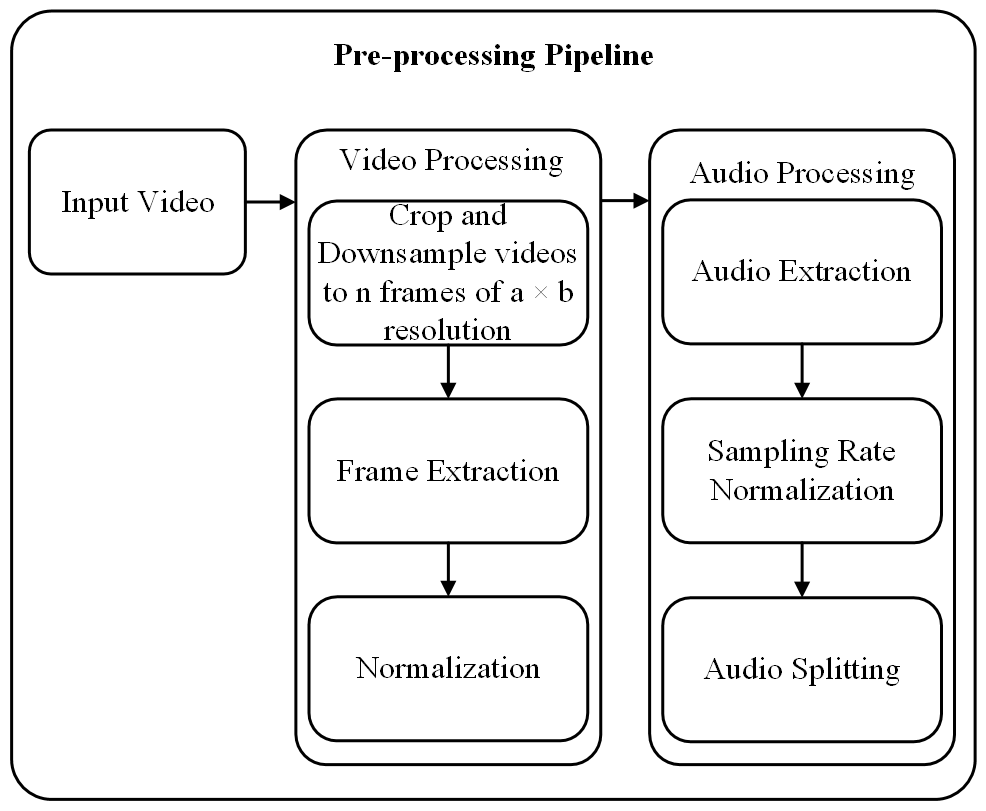
\includegraphics[width=0.9\linewidth]{assets/Major Data Pre-Processing.png}
            \caption{Pre-processing Pipeline}
            \label{fig:pre-processing-pipeline}
        \end{figure}
        
        \textbf{Overview of the Pre-processing Pipeline for Video with Audio}
        The figure illustrates a pre-processing pipeline designed for handling video files with accompanying audio tracks. The pipeline is organized into two main branches: one for processing video data and the other for audio data. Each branch standardizes and optimizes the respective data types, ensuring compatibility for integration and further analysis or processing.
        
        \textbf{Video Processing Branch}
        \begin{itemize}
            \item \textbf{Crop and Downsample Videos to \(n\) Frames of \(a \times b\) Resolution:} 
            Video frames are cropped and resized to a fixed resolution of \(a \times b\). This step reduces the complexity of the video data, making it computationally efficient while preserving essential visual information. Additionally, the video is downsampled to \(n\) frames, ensuring a uniform frame rate and minimizing redundancy.
        
            \item \textbf{Pixel Extraction:} 
            After downsampling, individual pixel values are extracted from each video frame. These pixel values represent the visual content of the video and encapsulate the color and intensity information for each frame.
        
            \item \textbf{Normalization:} 
            The extracted pixel values are normalized to a standard range, typically between 0 and 1. Normalization ensures consistency in data representation, minimizes numerical instability, and facilitates improved performance in subsequent processing stages.
        \end{itemize}
        
        \textbf{Audio Processing Branch}
        \begin{itemize}
            \item \textbf{Audio Extraction at Sample Rate \(a \times b\) kHz:} 
            The audio data is extracted from the input video and resampled to match the video resolution, specifically at a sample rate proportional to the resolution (\(a \times b\) kHz). This alignment ensures that the audio data corresponds directly to the spatial dimensions of the video frames.
        
            \item \textbf{Sampling Rate Normalization:} 
            The resampled audio undergoes normalization to standardize its amplitude range. This ensures uniformity in the audio data and aligns it with the normalized video pixel data.
        
            \item \textbf{Repeat Audio to Match the Number of Pixels:} 
            To synchronize the audio with the video data, audio samples are repeated so that their quantity matches the number of pixels in each video frame. This step ensures compatibility between the audio and video data for seamless integration and processing.
        \end{itemize}
        
        After pre-processing, the video and audio data are standardized and aligned for integration. The video frames with normalized pixel data and the corresponding audio samples are represented in a unified format. This unified representation ensures that the input data is prepared and ready for further processing, including model fitting and analysis.
        
        \subsubsection{Training Model (Fully Connected Neural Network)}
        A specially designed neural network consisting of multiple fully connected layers is trained to accept space-time coordinates as input and output the corresponding \gls{rgb} values for pixels and the amplitude for the audio, effectively mapping these inputs to their visual and auditory outputs.
    
        \subsubsection{Compression Pipeline}
        \begin{enumerate}[label=\textbf{\roman*.}]
            \item \textbf{Knowledge Distillation:} A smaller model is trained to mimic the behavior of a larger overfitted model, effectively transferring knowledge while reducing the complexity of the model.
            \item \textbf{16-bit Integer Quantization:} The network parameters are reduced in precision by quantizing them to 16-bit integers, which decreases the model size while retaining essential information and minimizing performance loss.
            \item \textbf{Model Encoding:} The quantized model weights are encoded using \gls{lzma}. This process compresses the quantized weights into a compact and efficient representation for transmission or storage.
        \end{enumerate}
        \subsubsection{Transmission and Decompression}

        After the model has been processed through the compression pipeline, it is transmitted over a guided or unguided channel to the receiving end. This transmission ensures that the compressed and encoded model reaches its destination efficiently, preserving the integrity of the compressed data.

        Once received, the model undergoes a decompression process, starting with \textbf{decoding}. In this step, the encoded data is converted back into its quantized format. The decoding process reverses the arithmetic or range encoding applied during the compression pipeline in \gls{lzma}, ensuring that the quantized weights and parameters are accurately restored.

        Following decoding, the model is passed through \textbf{dequantization}. During this step, the quantized data, represented as 16-bit integers, is scaled back to its original precision range. This scaling is achieved using the quantization parameters (such as scale and zero-point) that were preserved during the compression process. Dequantization restores the numerical accuracy of the model while maintaining the reduced size achieved through quantization.

        The decompressed model, now in its restored form, is ready for inference. At this stage, it provides RGB values for each pixel and amplitude values for audio corresponding to the space-time coordinates $\left[(x, y, t), T\right]$. These outputs serve as the foundation for the subsequent steps in the post-processing pipeline.'

        \subsubsection{Post-processing Pipeline}
        \begin{figure}[H]
            \centering
            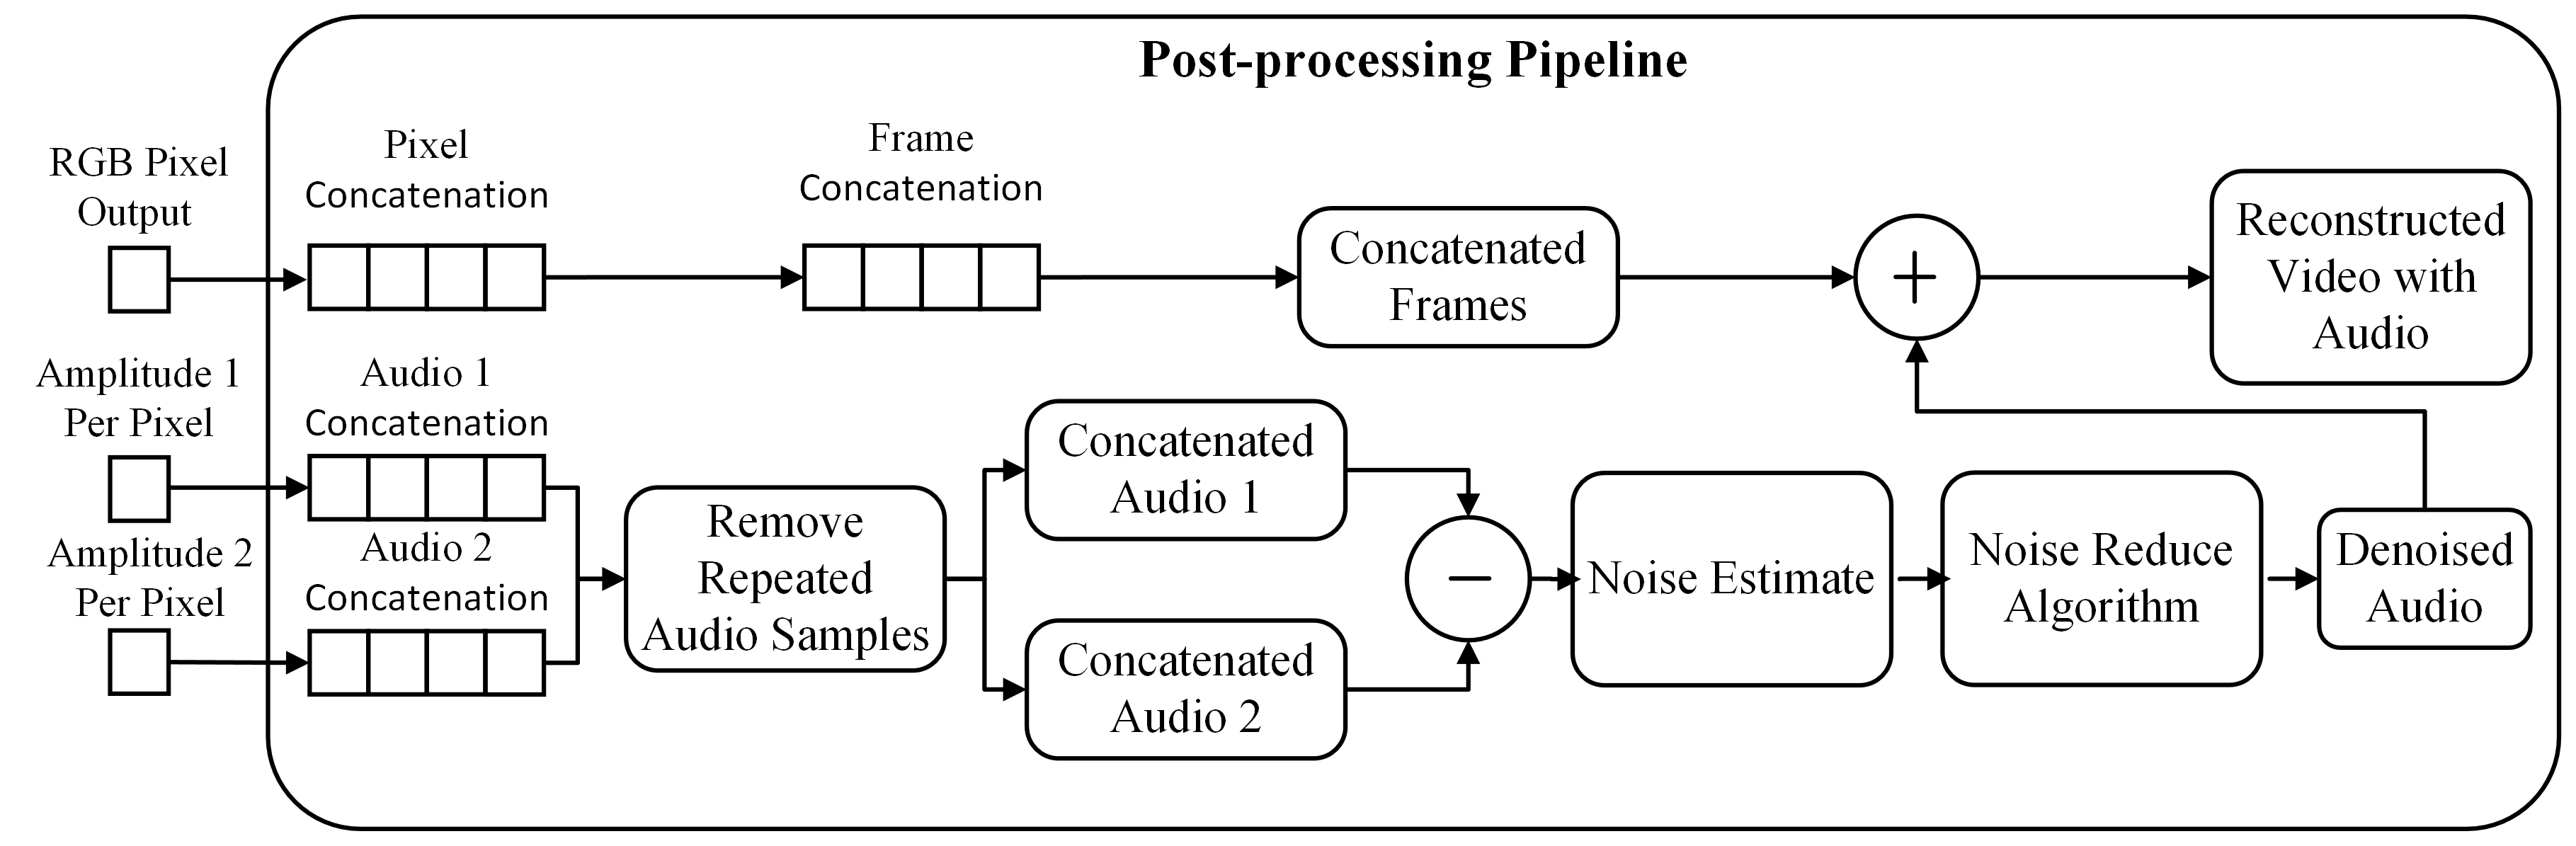
\includegraphics[width=0.9\linewidth]{assets/Major Data Post-Processing.png}
            \caption{Post-processing Pipeline}
            \label{fig:post-processing-pipeline}
        \end{figure}
        The post-processing pipeline illustrated in \autoref{fig:post-processing-pipeline} outlines the steps taken after the transmitted model has been decompressed and dequantized. The decompressed model is inferenced to retrieve the respective RGB values and audio amplitude values for the space-time coordinates $\left[(x, y, t), T\right]$. These outputs are critical for reconstructing the video and audio components.

        The RGB values for each pixel are extracted and concatenated into a tensor that represents the color information for the video frames. Similarly, the model outputs two amplitude values for the audio—Amplitude 1 and Amplitude 2—corresponding to each pixel. These amplitude values are concatenated to form a unified audio signal. However, the concatenated audio includes repeated samples, which are removed in the next step to match the original audio sample rate and timing. This ensures the audio remains synchronized with the video frames.
        
        To enhance the audio quality, a noise reduction process is performed. The two audio outputs (Concatenated Audio 1 and Concatenated Audio 2) are subtracted to estimate the noise present in the audio. The estimated noise, along with one of the audio outputs, is then passed through a noise reduction algorithm. This algorithm processes the signals to produce a denoised audio output that is free from distortions and artifacts.
        
        Meanwhile, the concatenated RGB values are used to generate individual video frames. These frames are then merged to reconstruct the full video. Finally, the denoised audio is combined with the reconstructed video to create the complete decompressed video with synchronized audio. This pipeline ensures a high-quality output with minimal noise and distortion, preserving the fidelity of the original input.
    \subsubsection{Noise Reduction Process}
    During the training and inference phases, the generated audio signals contained residual noise, which was due to imperfections in the model's processing. To address this, we applied a noise reduction algorithm specifically designed to suppress this residual noise while preserving the integrity of the audio content. The noise estimate was obtained by leveraging the two audio output branches, which generated two inferred outputs for the same signal; the difference between these outputs was used to estimate the noise. Using this noise estimate, a dedicated noise clip was extracted to compute noise characteristics such as mean and standard deviation across frequency bands. A dynamic noise threshold was then determined and applied to the audio spectrogram, followed by Gaussian smoothing to refine the noise suppression mask. This process effectively removed the residual noise and ensured the reconstructed audio maintained high fidelity.
    The following section details the implementation of this noise reduction algorithm.
    \begin{algorithm}[H]
        \caption{Noise Reduction Algorithm}
        \label{alg:noise_reduction}
        \begin{algorithmic}[1]
        \REQUIRE audio\_clip, noise\_clip, parameters (smoothing parameters, FFT size, and threshold control)
        
        \STATE \textbf{Compute Spectrogram of Noise:}
        \STATE noise\_stft $\gets$ \texttt{STFT(noise\_clip)}
        \STATE noise\_stft\_db $\gets$ \texttt{ConvertToDB(noise\_stft)}
        \STATE mean\_freq\_noise $\gets$ \texttt{Mean(noise\_stft\_db, axis=freq)}
        \STATE std\_freq\_noise $\gets$ \texttt{Std(noise\_stft\_db, axis=freq)}
        \STATE noise\_threshold $\gets$ mean\_freq\_noise + $k \times$ std\_freq\_noise
        
        \STATE \textbf{Compute Spectrogram of Audio:}
        \STATE sig\_stft $\gets$ \texttt{STFT(audio\_clip)}
        \STATE sig\_stft\_db $\gets$ \texttt{ConvertToDB(sig\_stft)}
        
        \STATE \textbf{Generate Mask:}
        \STATE sig\_mask $\gets$ (sig\_stft\_db $>$ noise\_threshold)
        \STATE smoothed\_mask $\gets$ \texttt{ApplyGaussianFilter(sig\_mask)}
        
        \STATE \textbf{Apply Mask:}
        \STATE masked\_stft $\gets$ sig\_stft $\times$ smoothed\_mask
        
        \STATE \textbf{Reconstruct Signal:}
        \STATE recovered\_signal $\gets$ \texttt{ISTFT(masked\_stft)}
        
        \RETURN recovered\_signal
        \end{algorithmic}
    \end{algorithm}
    
    \subsection{Quantization}
    \textit{Quantization} in machine learning is the process of reducing the number of bits that represent the model's weights and activations. It typically involves converting 32-bit floating-point numbers to lower precision formats like 16-bit, 8-bit, or even binary (1-bit) representations. This reduces the model size and accelerates inference on hardware with limited computational resources.

    \autoref{alg:model-quantization} outline the process of model quantization, which aims to reduce the precision of neural network weights to improve efficiency. The process begins with a trained neural network model. The first step is to choose a quantization scheme, which can be either uniform quantization, where weights are mapped to fixed, uniformly distributed levels, or non-uniform quantization, where techniques like k-means clustering are used to determine the mapping. Following this, the number of quantization levels $Q$ is determined (e.g., 8-bit, 16-bit). Each weight $W_{ij}$ in the model is then mapped to the nearest quantization level within $Q$. The original weights $W$ are replaced with these quantized weights, resulting in a quantized model. Optionally, the quantized model can be fine-tuned on the training dataset to recover any lost accuracy. The final step is to return the quantized model $Q(W)$. This approach effectively reduces the model's memory footprint and potentially improves its computational efficiency while maintaining its performance.
    
    \begin{algorithm}[H]
        \caption{Model Quantization}
        \label{alg:model-quantization}
        \begin{algorithmic}[1]
        \REQUIRE Neural network model with weights $W$, training dataset, quantization levels $Q$ (e.g., 8-bit, 16-bit)
        
        \STATE Train the model on the training dataset
        \STATE Find zero-point and scale factor for each layer
        \FOR{each weight $W_{ij}$ in $W$}
            \STATE Map $W_{ij}$ to the nearest quantization level in $Q$
        \ENDFOR
        \STATE Replace original weights $W$ with quantized weights $Q(W)$
        \STATE Also store the scale factor and zero-point for each layer
        
        \RETURN $Q(W)$
        \end{algorithmic}
    \end{algorithm}
        

    \subsection{Loss Function}
    To effectively generate \gls{inr} for audio-video data, it is essential to define appropriate loss functions that guide the learning process. Below, the specific loss functions for audio and video are introduced, followed by the formulation of a combined loss function that integrates both modalities.

        \subsubsection{Audio Loss Function}
        The loss function for audio data is defined as:
        \begin{equation}
            \mathcal{L}_{\text{audio}} = 0.5 \left( \int_{\Omega_{\text{audio}}} \| \Phi_{\text{audio,1}}(t) - f_{\text{audio}}(t) \| \, dt \right) + 0.5 \left( \int_{\Omega_{\text{audio}}} \| \Phi_{\text{audio,2}}(t) - f_{\text{audio}}(t) \| \, dt \right)
        \end{equation}
        where,
        \begin{itemize}
            \item \( t \in \mathbb{R} \) is the time point,
            \item  \( \Phi_{\text{audio,1}}(t) \) is the first audio output of the model at time \( t \),
            \item \( \Phi_{\text{audio,2}}(t) \) is the second audio output of the model at time \( t \),
            \item \( f_{\text{audio}}(t) \) is the ground truth audio amplitude at time \( t \),
            \item \( \Omega_{\text{audio}} \) is the time interval over which the audio is defined.
        \end{itemize}
    
        \subsubsection{Video Loss Function}
            The loss function for video data is defined as:
        \begin{equation}
            \mathcal{L}_{\text{video}} = \int_{\Omega_{\text{video}}} \| \Phi_{\text{video}}(x, t) - f_{\text{video}}(x, t) \| \, dx \, dt
        \end{equation}
        where,
        \begin{itemize}
        \item \( (x, t) \in \mathbb{R}^3 \) represents the space-time coordinates,
        \item \( \Phi_{\text{video}}(x, t) \) is the model's output for the video at space-time coordinate \( (x, t) \),
        \item \( f_{\text{video}}(x, t) \) is the ground truth RGB value at space-time coordinate \( (x, t) \),
        \item \( \Omega_{\text{video}} \) is the space-time region over which the video is defined.
        \end{itemize}
    
        \subsubsection{Combined Teacher Loss Function}
        The combined loss function for both audio and video data is formulated as:
        \begin{equation}
            \mathcal{L}_{\text{combined}} = \lambda_{\text{audio}} \mathcal{L}_{\text{audio}} + \lambda_{\text{video}} \mathcal{L}_{\text{video}}
            \end{equation}
            where,
            \begin{itemize}
                \item \( \lambda_{\text{audio}} \) is the weight that balances the contribution of the audio loss,
                \item \( \lambda_{\text{video}} \) is the weight that balances the contribution of video loss.
            \end{itemize}
    This combined loss function ensures that both the audio and video outputs are supervised and optimized simultaneously.

    \subsubsection{Knowledge Distillation Loss Function}
    The Knowledge Distillation (KD) loss function is formulated to combine both the hard and soft loss components for audio and video data. The overall loss is defined as:

    \begin{equation}
        \mathcal{L}_{\text{KD}} = \alpha \mathcal{L}_{\text{hard}} + (1 - \alpha) \mathcal{L}_{\text{soft}}
    \end{equation}
    where,

    \begin{itemize}
        \item \( \alpha \) is a hyperparameter that balances the contribution of the hard and soft loss components,
        \item \( \mathcal{L}_{\text{hard}} \) is the total hard loss (based on the student's output and the ground truth),
        \item \( \mathcal{L}_{\text{soft}} \) is the total soft loss (based on the student's output and the teacher's output).
    \end{itemize}

    The hard and soft losses are defined as:

    \begin{equation}
        \mathcal{L}_{\text{hard}} = 0.5 \times \mathcal{L}_{\text{video, hard}} + 0.5 \times \left( 0.5 \times \mathcal{L}_{\text{audio, hard}} + 0.5 \times \mathcal{L}_{\text{audio(siam), hard}} \right)
    \end{equation}

    \begin{equation}
        \mathcal{L}_{\text{soft}} = 0.5 \times \mathcal{L}_{\text{video, soft}} + 0.5 \times \left( 0.5 \times \mathcal{L}_{\text{audio, soft}} + 0.5 \times \mathcal{L}_{\text{audio(siam), soft}} \right)
    \end{equation}

    
    \subsection{Evaluation Metrics for Video}
        To rigorously evaluate the effectiveness of our proposed INR based video compression technique, we will utilize a suite of metrics that assess various dimensions of video quality, including visual fidelity, perceptual quality, and predictive accuracy. Here's an overview of each metric, their numerical value ranges, and whether it's preferable for their values to increase or decrease:
        \subsubsection{Peak Signal-to-Noise Ratio}
            \begin{itemize}
                \item \textbf{Overview}: \gls{psnr} is commonly employed to measure the quality of reconstruction in lossy compression \gls{codec}s. It compares the similarity between the original and compressed video by measuring the ratio between the maximum possible power of a signal and the power of distorting noise.
                \item \textbf{Value Range}: Typically expressed in \gls{db}, the higher the \gls{psnr}, the better the quality of the compressed video. A higher \gls{psnr} value indicates that the reconstruction is of higher quality.
                \item \textbf{Preference} $\uparrow$: Values typically range from 20 to 50 \gls{db}, where higher values (around 40 \gls{db} or more) represent excellent quality.
                \item \textbf{Formula}
                \begin{equation}\label{eqn:PSNR}
                    \text{PSNR} = 20 \cdot \log_{10}\left(\frac{{\text{MAX}_I}}{\sqrt{\text{MSE}}}\right)
                \end{equation}
                where, $\text{MAX}_I$ is the maximum possible pixel value of the image (e.g., 255 for 8-bit images), and $\text{MSE}$ is the mean squared error between the original and compressed image.
               \end{itemize} 

        \subsubsection{Signal-to-Quantization Noise Ratio (SQNR)}
        \label{subsubsec:SQNR}
        \begin{itemize}
            \item \textbf{Overview}: \gls{sqnr} is a widely used metric to assess the quality of quantized signals in digital signal processing and machine learning models. It measures the ratio of the power of the original signal to the power of the noise introduced during quantization.
            \item \textbf{Value Range}: Typically expressed in \gls{db}, higher \gls{sqnr} values indicate better fidelity of the quantized signal to the original. A perfect quantization would result in an infinite \gls{sqnr}.
            \item \textbf{Preference} $\uparrow$: Higher values are preferred, as they represent lower quantization noise. For practical systems, values depend on the bit depth and dynamic range of the quantizer.
            \item \textbf{Formula}
            \begin{equation}\label{eqn:SQNR}
                \text{SQNR} = 10 \cdot \log_{10}\left(\frac{P_s}{P_n}\right)
            \end{equation}
            where, \(P_s\) is the signal power, defined as:
            \begin{equation}
                P_s = \frac{1}{N} \sum_{i=1}^N x_i^2
            \end{equation}
            and \(P_n\) is the quantization noise power, defined as:
            \begin{equation}
                P_n = \frac{1}{N} \sum_{i=1}^N (x_i - \hat{x}_i)^2
            \end{equation}
            Here, \(x_i\) is the original signal, \(\hat{x}_i\) is the quantized signal, and \(N\) is the number of samples.
        \end{itemize}
               
           
        \subsubsection{Learned Perceptual Image Patch Similarity}
            \begin{itemize}
                \item \textbf{Overview}: \gls{lpips} metric evaluates the perceptual difference between two images or videos. Unlike traditional metrics that focus on pixel-level accuracy, \gls{lpips} uses deep learning to assess how perceptually similar two images are to the human eye.
                \item \textbf{Value Range}: This metric produces a similarity score that ranges from 0 to 1, where lower scores indicate greater perceptual similarity.
                \item \textbf{Preference} $\downarrow$: A lower \gls{lpips} score means that the compressed video is perceptually closer to the original, indicating better compression performance.
            \end{itemize}

        \subsubsection{Structural Similarity Index Measure}
            \begin{itemize}
                \item \textbf{Overview}: \gls{ssim} is used to measure the similarity between two images or videos. It considers attributes that are important to the human visual system such as luminance, contrast, and structure.
                \item \textbf{Value Range}: \gls{ssim} values range from -1 to 1. A score of 1 indicates perfect similarity, meaning there is no loss of structural information.
                \item \textbf{Preference} $\uparrow$: Higher \gls{ssim} values signify less visual distortion and better compression quality.
                \item \textbf{Formula}
                \begin{equation}\label{eqn:SSIM}
                    \text{SSIM}(x, y) = \frac{(2 \mu_x \mu_y + c_1)(2 \sigma_{xy} + c_2)}{(\mu_x^2 + \mu_y^2 + c_1)(\sigma_x^2 + \sigma_y^2 + c_2)}
                \end{equation}
                where, $\mu_x$ and $\mu_y$ are the average intensities of images $x$ and $y$, $\sigma_{x}$ and $\sigma_y$ are the variance, $\sigma_{xy}$ is the covariance between $x$ and $y$, and $c_1$ and $c_2$ are variables to stabilize division.
            \end{itemize}

        \subsubsection{File Size}
            \begin{itemize}
                \item \textbf{Overview}: File size measures the total amount of storage space required by a compressed video file. It is a direct indicator of the efficiency of a compression technique.
                \item \textbf{Value Range}: File size is typically measured in bytes, \gls{kb}, \gls{mb}, or \gls{gb}. The value range can vary widely depending on the length and resolution of the video.
                \item \textbf{Preference} $\downarrow$: Lower file sizes are preferable as they indicate more efficient compression.
            \end{itemize}

        \subsubsection{Bandwidth Usage}
            \begin{itemize}
                \item \textbf{Overview}: Bandwidth usage measures the amount of data transmitted over a network to stream or download a video. It evaluates the feasibility of video transmission in various network conditions.
                \item \textbf{Value Range}:  Bandwidth usage is typically measured in \gls{bps}, \gls{kbps}, or \gls{mbps}. The value range can vary depending on the video quality and compression efficiency.
                \item \textbf{Preference} $\downarrow$: Lower bandwidth usage is preferable as it indicates more efficient data transmission.
            \end{itemize}

        \subsubsection{Encoding/Decoding Time}
        \begin{itemize}
            \item \textbf{Overview}: Encoding/decoding time measures the time required to compress (encode) or decompress (decode) a video file. It is a critical factor in real-time applications and systems with limited processing capabilities.
            \item \textbf{Value Range}: Encoding/decoding time is typically measured in seconds or milliseconds. The exact value can vary widely depending on the complexity of the video content.
            \item \textbf{Preference} $\downarrow$: Lower encoding/decoding times are preferred, as they indicate more efficient compression.
        \end{itemize}
\subsection{Evaluation Metrics for Audio}
To thoroughly assess the effectiveness of our proposed audio processing techniques, we will utilize a comprehensive suite of metrics that evaluate various aspects of audio quality, including clarity, fidelity, intelligibility, and perceptual similarity. Here's an overview of each metric, their numerical value ranges, and the preferred direction for their values:

\subsubsection{Log Spectral Distance (LSD)}
\begin{itemize}
    \item \textbf{Overview:} \gls{lsd} measures the difference between the log magnitude spectra of the reference and processed audio signals, making it sensitive to spectral distortions.
    
    \item \textbf{Value Range:} \gls{lsd} is typically measured in decibels (dB) and can range from 0 (no spectral distortion) to higher positive values.
    
    \item \textbf{Preference $\downarrow$:} Lower values are preferable, indicating lower spectral distortion.
    
    \item \textbf{Formula:}
    
    LSD is computed as:
    \begin{equation}
        \text{LSD} = \frac{1}{N} \sum_{n=1}^{N} \sqrt{\frac{1}{K} \sum_{k=1}^{K} \left[ \log |X(k,n)| - \log |Y(k,n)| \right]^2}
    \end{equation}
    where, \( X(k,n) \) and \( Y(k,n) \) are the magnitude spectra of the original and processed signals for the \( n \)-th frame and \( k \)-th frequency bin, respectively, \( N \) is the number of frames, and \( K \) is the number of frequency bins.
\end{itemize}

\subsubsection{Peak Signal-to-Noise Ratio (PSNR)}
\begin{itemize}
    \item \textbf{Overview:} \gls{psnr} is a widely used metric to measure the quality of reconstruction of lossy compression codecs. It represents the ratio between the maximum possible power of a signal and the power of corrupting noise.
    
    \item \textbf{Value Range:} \gls{psnr} is expressed in decibels (dB) and typically ranges from 20 to 50 dB, with higher values indicating better quality.
    
    \item \textbf{Preference $\uparrow$:} Higher values are preferable, indicating less noise and better signal reconstruction quality.
    
    \item \textbf{Formula:}
    
    PSNR is calculated as:
    \begin{equation}
        \text{PSNR} = 20 \cdot \log_{10}\left(\frac{{\text{MAX}_I}}{\sqrt{\text{MSE}}}\right)
    \end{equation}
    where, \( \text{MAX} \) is the maximum possible pixel value (in audio, the signal's peak value), and \gls{mse} is the mean squared error between the original and processed audio signals.
\end{itemize}

\subsubsection{Virtual Speech Quality Objective Listener (VISQOL)}

\begin{itemize}
    \item \textbf{Overview:} \gls{visqol} is an objective, full-reference metric for perceived audio quality. It uses a spectro-temporal measure of similarity between a reference and a test speech signal to produce a MOS-LQO (Mean Opinion Score - Listening Quality Objective) score. MOS-LQO scores range from 1 (the worst) to 5 (the best).

    \item \textbf{Value Range:} \gls{visqol} scores typically range from \textbf{1 to 5}, where \textbf{1} indicates poor perceived quality and \textbf{5} represents near-perfect audio quality.

    \item \textbf{Preference} $\uparrow$: Higher \gls{visqol} values are preferable, as they indicate better perceptual audio quality and closer resemblance to the original signal.

    \item \textbf{Formula:} \\
    \gls{visqol} is computed using a \textit{similarity index} between the original and processed audio signals. The process involves:
    \begin{enumerate}
        \item Computing frame-level perceptual similarities using frequency representations of the signals.
        \item Aggregating these similarities into a single perceptual quality score.
    \end{enumerate}
\end{itemize}

\subsubsection{File Size}
            \begin{itemize}
                \item \textbf{Overview}: File size measures the total amount of storage space required by a compressed video file. It is a direct indicator of the efficiency of a compression technique.
                \item \textbf{Value Range}: File size is typically measured in bytes, \gls{kb}, \gls{mb}, or \gls{gb}. The value range can vary widely depending on the length and resolution of the video.
                \item \textbf{Preference} $\downarrow$: Lower file sizes are preferable as they indicate more efficient compression.
            \end{itemize}


    \pagebreak

\section{\MakeUppercase{Dataset Exploration}}

\autoref{tab:audio_video_files} provides a summary of various audio-video files, detailing their serial numbers (SN), file names, resolution, frames per second (fps), audio sample rate,file size in \gls{mib} and video duration in seconds. All the audio-video files are stored in AVI/wav format because AVI is an uncompressed format that preserves the original, raw audio-video quality without any loss of data. Unlike compressed video formats, which reduce file size by discarding some visual information, AVI/wav files maintain the full integrity of audio-video streams.

\begin{table}[H]
    \centering
    \caption{Video Files Characteristics}
    \label{tab:audio_video_files}
    \begin{tabular}{|c|c|c|c|c|c|c|}
        \hline
        \multirow{2}{*}{\textbf{SN}} & \textbf{Video} & \multirow{2}{*}{\textbf{Resolution}} & \multirow{2}{*}{\textbf{FPS}} & \multicolumn{1}{c|}{\textbf{Sample}} & \multicolumn{1}{c|}{\textbf{Size}} & \multicolumn{1}{c|}{\textbf{Duration}} \\ 
        &\textbf{File} & & & \textbf{Rate (Hz)} & \textbf{(MiB)} & \textbf{(s)} \\ 
        \hline 
        1 & Video 1 & \multirow{5}{*}{448 x 256} & 1 & 114688 & 1.92 & 5 \\ 
        \cline{1-2} \cline{4-7}
        2 & Video 2 & & 1 & 96000 & 5.33 & 10 \\ 
        \cline{1-2} \cline{4-7}
        3 & Video 3 & & 10 & 114688 & 6.08 & 3 \\ 
        \cline{1-2} \cline{4-7}
        4 & Video 4 & & 2 & 114688 & 13.6 & 25 \\ 
        \cline{1-2} \cline{4-7}
        5 & Video 5 & & 24 & 114688 & 12.4 & 3 \\ 
        \hline
    \end{tabular}
\end{table}

Videos 1 and 2 contain temporally uncorrelated frames, selected to assess the model's performance when successive frames undergo significant changes. In Video 1, the audio features a melody played on the violin, with frequency components ranging from 1.60 Hz to 4437.80 Hz, while Video 2 includes the voice of a Nepali male speaker, whose audio spans a frequency range of 0.3 Hz to 5739.9 Hz.

On the other hand, Videos 3, 4, and 5 consist of temporally correlated frames and were chosen to evaluate how the model handles sequentially related data. Video 3 showcases a man dancing, accompanied by a song with audio frequencies spanning 0.1 Hz to 15537.67 Hz. Similarly, Video 4 involves people dancing with funky beats, and its audio frequency components range from 0.4 Hz to 10340.8 Hz. Video 5 presents a person delivering a speech in English, with its audio frequency range being 1.2 Hz to 10512.67 Hz.

The audio sample rates are set higher to accommodate the model's need for pixel coordinates, frame indices, and audio time steps as inputs. Given that the number of pixel coordinates is typically larger than the number of audio time steps, repeating the audio time steps to match the resolution would introduce significant repetition. To minimize this repetition and improve model performance, a higher sample rate is used.



\pagebreak

\section{\MakeUppercase{Implementation Details}}
The project is developed using Python, leveraging PyTorch as the primary deep learning framework. Interactive Python sessions are utilized for testing and rapid prototyping. Jupyter Notebooks are employed for exploratory data analysis and iterative experimentation, allowing for an interactive and visual approach to model development. TensorBoard is used to visualize training metrics and monitor the performance of the \gls{siren} network during training. Visual Studio Code serves as the main \gls{ide} for code writing and debugging.

\subsection{Instrumentation}
    The software and hardware used for this project are listed below:
    \begin{table}[H]
        \caption{Instrumentation Table}
        \label{table:instrumentation-table}
        \centering
        \begin{tabular}{|L{0.2\linewidth}|L{0.3\linewidth}|L{0.4\linewidth}|}
            \hline
            \textbf{Requirement} & \textbf{Solution} & \textbf{Reason} \\
            \hline
            High-Performance Computing & NVIDIA RTX 4090 & Overfitting the video to the model \\
            \hline
            Deep Learning Frameworks & PyTorch &
            Developing and implementing neural network models \\
            \hline
            Development Environment & Visual Studio Code with Notebook extensions & Running and Debugging Code\\
            \hline
        \end{tabular}
    \end{table}
    


\subsubsection{Hardware Specifications}
The project is trained on a system with the following specifications:
    \begin{itemize}
        \item \textbf{CPU:} The system is equipped with a 13th Gen Intel® Core™ i9-13980HX processor, featuring 32 cores with a base clock speed of 2.42 GHz. This provides substantial computational power for training deep learning models.
        \item \textbf{GPU:} The primary \gls{gpu} is an NVIDIA GeForce RTX 4090 Laptop \gls{gpu} with 16 \gls{gib} of VRAM, which accelerates the training and inference processes of the \gls{siren} network. This powerful \gls{gpu} is crucial for handling the complex computations required for video compression tasks.
        \item \textbf{Memory:} The system has a total of 24 \gls{gib} of RAM, ensuring ample memory for handling large datasets and complex models during training and evaluation.
    \end{itemize}




\subsection{Neural Network Architecture (Audio + Video)}
\begin{figure}[H]
    \centering
    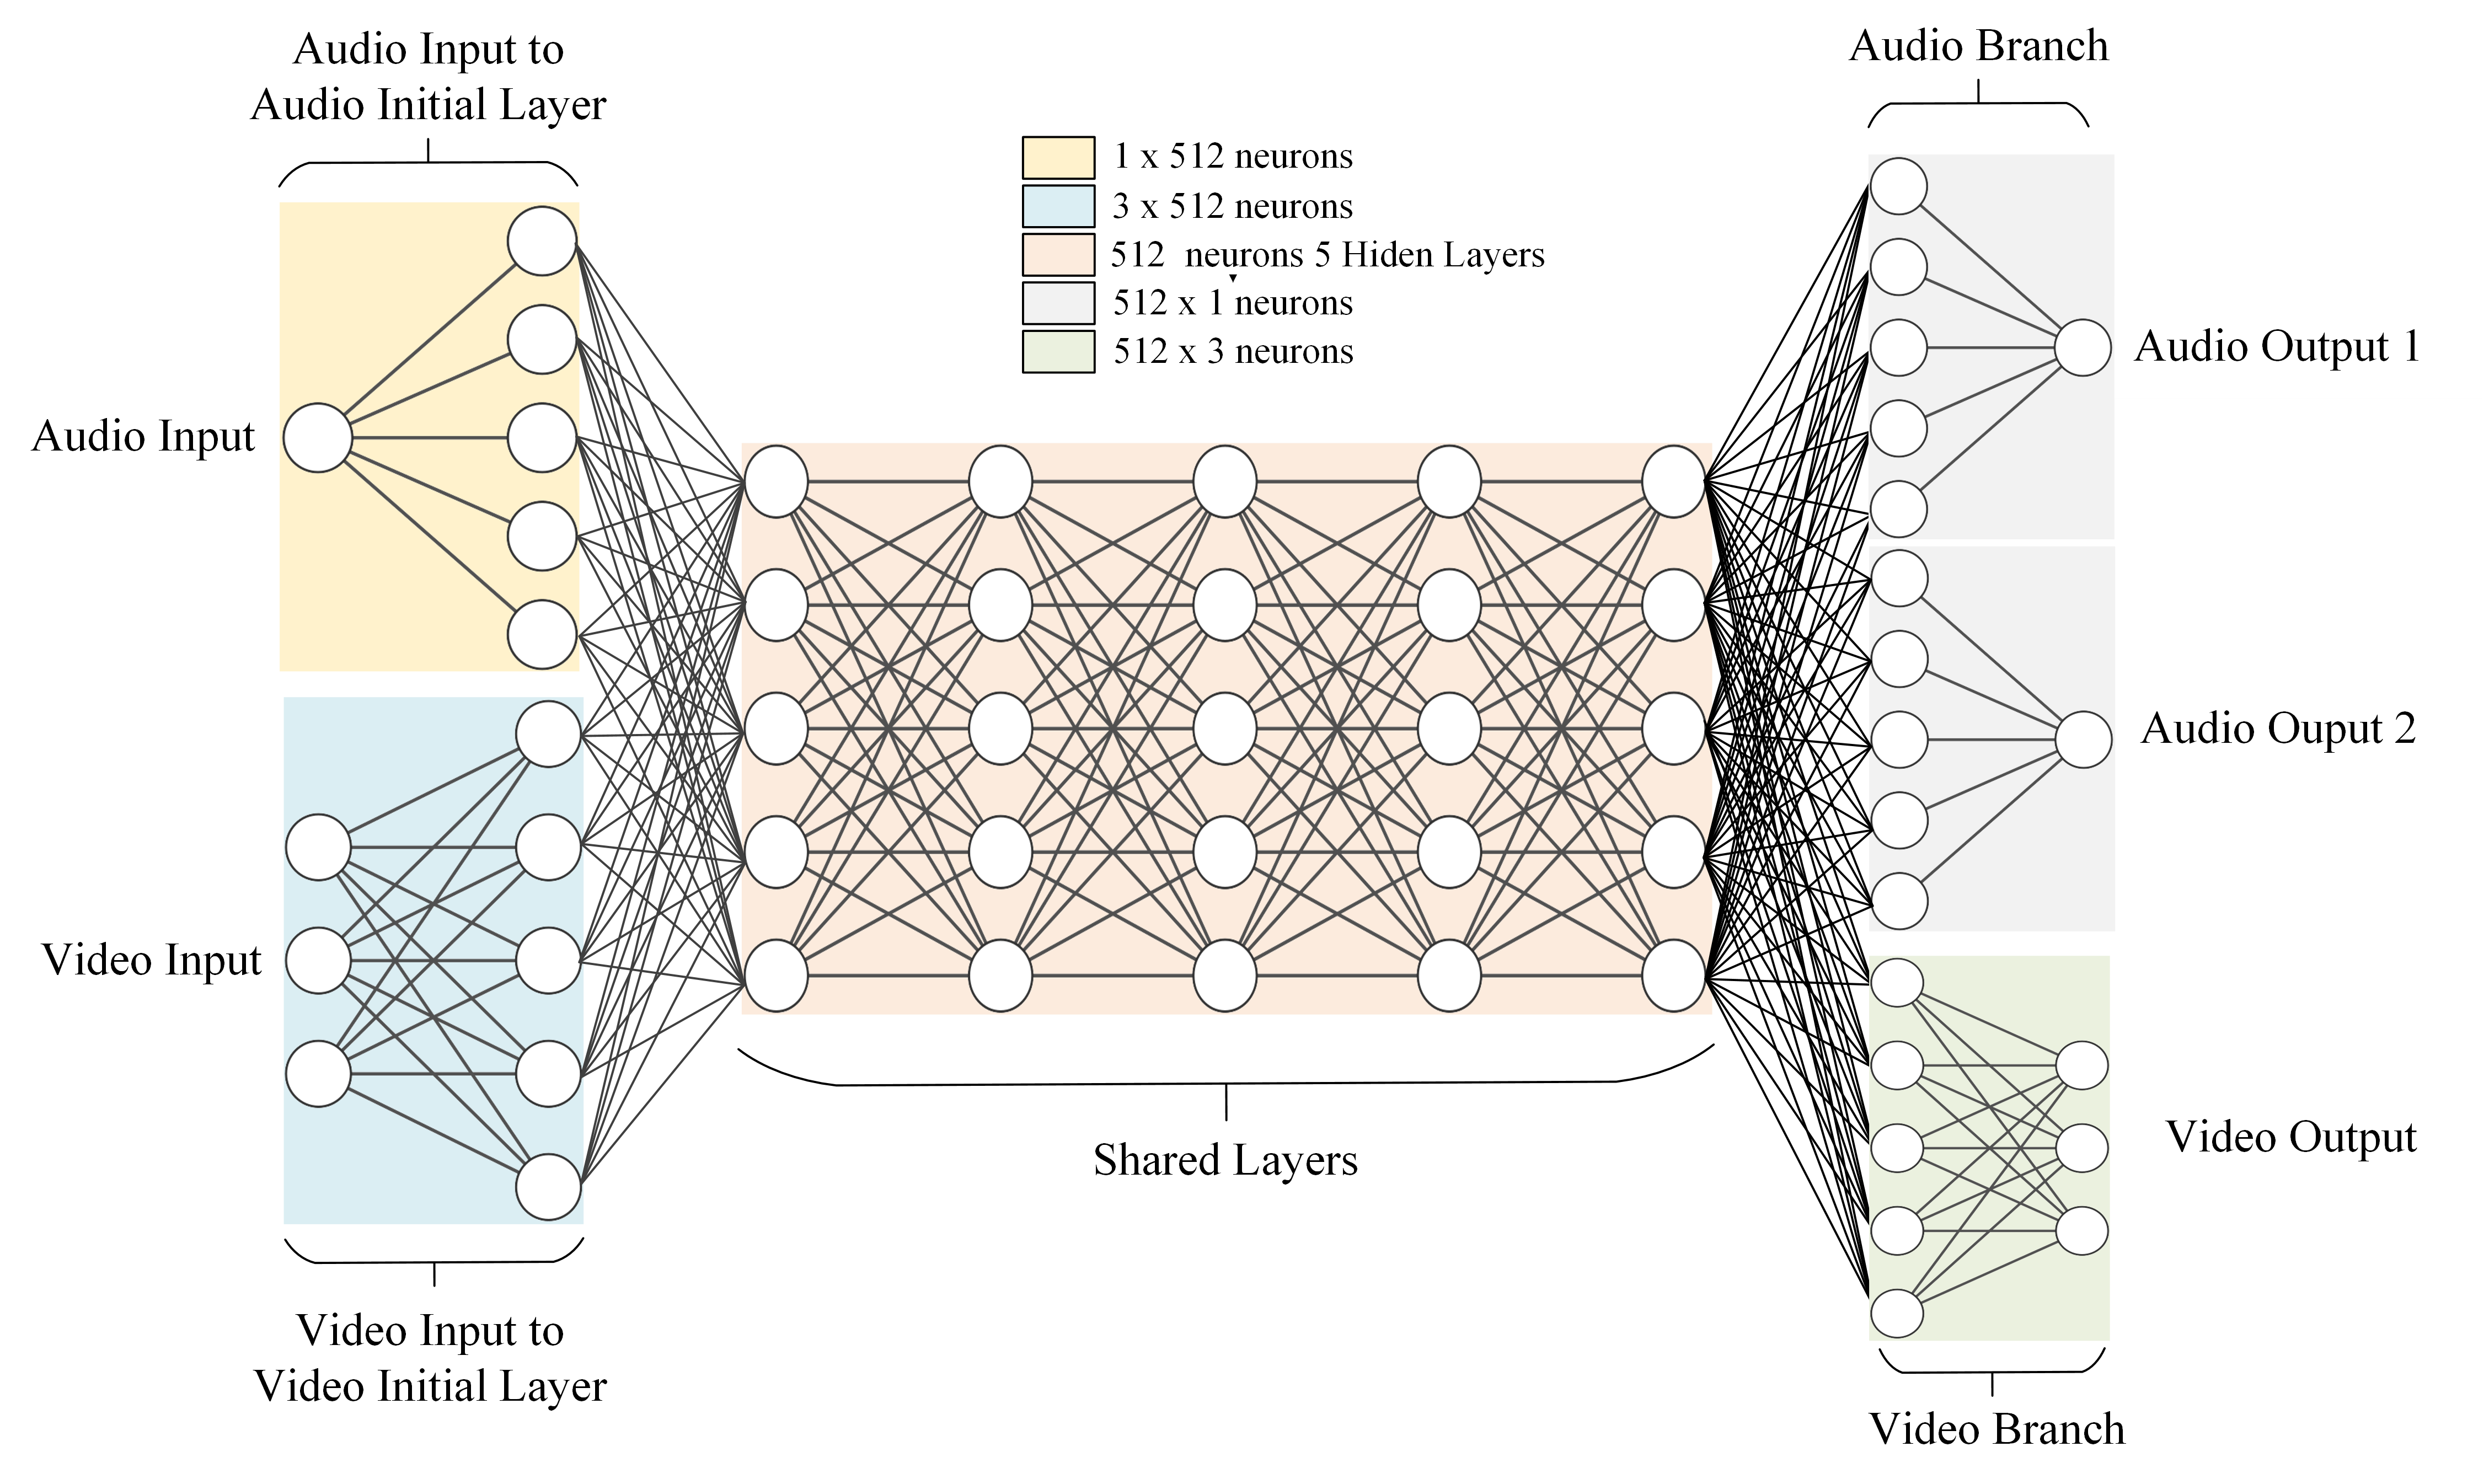
\includegraphics[width=\linewidth]{assets/audio_video_neural.png}
    \caption{SIREN Architecture for Video with Audio}
    \label{fig:arch-audio}
\end{figure}

The \gls{siren} architecture for video with audio consists of three major components: the initial layers, the shared layers, and the video/audio branches. The input to the network includes the spatial-temporal coordinates \(x, y, t\), the frame index \(t\), and the audio timestep \(T\), while the output consists of the RGB pixel values and the audio amplitude \(A\).

The input \(T\) is passed to the audio initial branch and the  spatial-temporal input \(x, y, t\) is fed into the video initial branch. The outputs from these initial layers are then combined and sent to the shared layers, which consist of five layers for the teacher model and three layers for student.

The output from the shared layers is branched into three separate layers: two branches for audio and one for video. The two audio branches are identical, each comprising one layer, which  is a linear layer. These two branches each produce slightly different amplitudes \(A\) for the same audio timestep \(T\), and these outputs are used to estimate and remove noise from the audio data. The video branch consists of one layer as well, being a linear layer, whose output is the RGB values.

The distinct initial layers for audio and video are necessary because it is not possible to have a good initialization for both audio and video if they were in the same branch. The audio branch works well with weights initialized within the range \([-25, 25]\), and the video branch performs well with weights initialized in the range \([-2/3, 2/3]\). Therefore, separate initial layers are required to optimize the reconstruction quality for both modalities.

The two identical audio branches are crucial because they provide the necessary outputs for noise estimation and removal from the audio data. All hidden layers in the shared and initial branches consist of 512 neurons for teacher model while all layers except hidden layers consists of 300 neurons with hidden layers consisting of 512 neurons for student model, with sine activations, except for the last layers in the two audio output branches and the video output branch, which uses linear activation.

\subsubsection{Trainable Parameters}
The breakdown of the trainable parameters (weights and biases) are as follows:

\begin{table}[H]
    \caption{Trainable Parameters in the SIREN Models}
    \label{table:trainable-parameters-teacher-student}
    \centering
    \resizebox{\textwidth}{!}{
    \begin{tabular}{|p{6em}|l|c|c|c|c|}
    \hline
    \multirow{2}{*}{\textbf{Layer}}             & \multirow{2}{*}{\textbf{Parameter}}             & \multicolumn{2}{c|}{\textbf{Dimensions}} & \multicolumn{2}{c|}{\textbf{Total}} \\ \cline{3-6}
                                  &                                  & \textbf{Teacher}    & \textbf{Student}    & \textbf{Teacher}    & \textbf{Student}    \\ \hline
    \multirow{2}{8em}{\textbf{Audio Initial Branch}} & Weight matrix                   & $1 \times 512$      & $1 \times 300$      & 512                 & 300                 \\
                                  & Bias vector                     & $512$               & $300$               & 512                 & 300                 \\ \hline
    \multirow{2}{8em}{\textbf{Video Initial Branch}} & Weight matrix                   & $3 \times 512$      & $3 \times 300$      & 1,536               & 900                 \\
                                  & Bias vector                     & $512$               & $300$               & 512                 & 300                 \\ \hline
    \multirow{2}{5em}{\textbf{Shared Layers}}        & Weight matrix                   & $1024 \times 512$   & $600 \times 512$    & 524,288             & 307,200             \\
                                  & Bias vector                     & $512$               & $512$               & 512                 & 512                 \\
                                  & Weight matrix        & $4 \times (512 \times 512)$    & $2 \times (512 \times 512)$ & 1,048,576     & 524,288            \\
                                  & Bias vector         & $4 \times 512$      & $2 \times 512$      & 2,048               & 1,024              \\ \hline
    \multirow{2}{5em}{\textbf{Video Branch}}         & Weight matrix                   & $512 \times 512$    & $512 \times 300$    & 262,144             & 153,600             \\
                                  & Bias vector                     & $512$               & $300$               & 512                 & 300                 \\
                                  & Weight matrix                   & $512 \times 3$      & $300 \times 3$      & 1,536               & 900                 \\
                                  & Bias vector                     & $3$                 & $3$                 & 3                   & 3                   \\ \hline
    \multirow{2}{5em}{\textbf{Audio Branch 1}}       & Weight matrix                   & $512 \times 512$    & $512 \times 300$    & 262,144             & 153,600             \\
                                  & Bias vector                     & $512$               & $300$               & 512                 & 300                 \\
                                  & Weight matrix                   & $512 \times 1$      & $300 \times 1$      & 512                 & 300                 \\
                                  & Bias vector                     & $1$                 & $1$                 & 1                   & 1                   \\ \hline
    \multirow{2}{5em}{\textbf{Audio Branch 2}}       & Weight matrix                   & $512 \times 512$    & $512 \times 300$    & 262,144             & 153,600             \\
                                  & Bias vector                     & $512$               & $300$               & 512                 & 300                 \\
                                  & Weight matrix                   & $512 \times 1$      & $300 \times 1$      & 512                 & 300                 \\
                                  & Bias vector                     & $1$                 & $1$                 & 1                   & 1                   \\ \hline
    \multicolumn{4}{|c|}{\textbf{Total}}  & \textbf{2,369,029}  & \textbf{1,298,029} \\ \hline
    \end{tabular}
    }
\end{table}


The total number of trainable parameters in the neural network is 2,369,029 for teacher model and 1,298,029 for student model.

\subsubsection{Hyperparameters for the Model}
\begin{table}[H]
    \centering
    \caption{Hyperparameters for Training the Teacher and Student Models}
    \begin{tabular}{|l|p{0.2\textwidth}|p{0.3\textwidth}|}
    \hline
    \textbf{Hyperparameter ($\boldsymbol{\theta}$)} & \textbf{Teacher Model} & \textbf{Student Model}  \\
    \hline
    Number of Epochs                   & 7000                    & 6000                    \\
    \hline
    \multicolumn{1}{|l|}{Omega ($\omega$)} & \multicolumn{2}{c|}{30}  \\
    \hline
    \multicolumn{1}{|l|}{First Layer Weight (Audio) ($\beta_a$)} & \multicolumn{2}{c|}{$(-25, 25)$} \\
    \hline
    \multicolumn{1}{|l|}{First Layer Weight (Video) ($\beta_v$)} & \multicolumn{2}{c|}{$\left(-\frac{2}{3}, \frac{2}{3}\right)$} \\
    \hline
    Learning Rate ($\eta$)              & $1\times10^{-5}$       & $1\times10^{-4}$ for the first 1000 epochs, $1\times10^{-5}$ for the remaining 5000 epochs \\
    \hline
    \multicolumn{1}{|l|}{Optimizer ($\text{Opt}$)} & \multicolumn{2}{c|}{Adam} \\
    \hline
    \end{tabular}
    \label{tab:teacher_student_model_hyperparams}
\end{table}
    
The model was trained for 7000 epochs for the teacher model and 6000 epochs for the student model, with the best-performing version saved based on the lowest loss achieved during training. The value of $\omega$ was set to 30 for both models, following the default configuration of the \gls{siren}model, as it effectively balances frequency representation.

For the first layer weight initialization, the audio branch used a range of $(-25, 25)$ ($\beta_a$) for both the teacher and student models. This range was specifically chosen to accurately represent high-frequency audio features while avoiding unnecessary noise. Larger ranges were tested but resulted in excessive noise, making $(-25, 25)$ the ideal choice.

Similarly, the video branch utilized a narrower initialization range of $\left(-\frac{2}{3}, \frac{2}{3}\right)$ ($\beta_v$) for both models, reflecting the lower frequency nature of video data. Wider ranges led to grainy images and inaccurate color predictions, confirming this range as optimal.

The learning rate was set to $1 \times 10^{-5}$ ($\eta$) for the teacher model and $1 \times 10^{-4}$ for the first 1000 epochs, then $1 \times 10^{-5}$ for the remaining 5000 epochs for the student model, ensuring stable and gradual optimization without large fluctuations in the loss function. The Adam optimizer ($\text{Opt}$) was employed for both models, due to its suitability for SIREN-based models, leveraging its adaptive learning capabilities to efficiently handle sinusoidal feature extraction and optimize the model effectively.

\pagebreak

\subsection{Data Preparation and Training Implementation}

\subsubsection{Pseudocode for Data Preparation}

\autoref{alg:synchronize_video_audio} ensures that the total number of video pixels and corresponding audio samples are synchronized for input compatibility with the model, which requires inputs in the format \([(x, y, t), T]\). 

If the number of video samples (\texttt{video\_size}) is less than the number of audio samples (\texttt{audio\_size}), the algorithm repeats the video coordinates and data until they match the audio sample count. The repetition is performed by calculating a repeat factor as the integer division of \texttt{audio\_size} by \texttt{video\_size}, and appending any remaining samples as needed. 

Similarly, if the audio sample count is smaller, the audio coordinates and data are repeated to align with the video sample count. The process ensures that both video and audio inputs are synchronized and ready for processing by the model.

The synchronized outputs are returned as \texttt{video\_coords}, \texttt{video\_data}, \texttt{audio\_coords}, and \texttt{audio\_data}.

\begin{algorithm}
    \caption{Synchronize Video and Audio Samples}
    \label{alg:synchronize_video_audio}
    \begin{algorithmic}[1]
    \REQUIRE video\_coords, video\_data, audio\_coords, audio\_data
    \STATE video\_size $\gets$ Number of video samples
    \STATE audio\_size $\gets$ Number of audio samples
    \IF{video\_size \textless\ audio\_size}
        \STATE repeat\_factor $\gets \lfloor$ audio\_size / video\_size $\rfloor$
        \STATE remainder $\gets$ audio\_size mod video\_size
        \STATE Repeat video coordinates and data by repeat\_factor
        \IF{remainder \textgreater\ 0}
            \STATE Append first remainder video samples
        \ENDIF
    \ELSIF{audio\_size \textless\ video\_size}
        \STATE repeat\_factor $\gets \lfloor$ video\_size / audio\_size $\rfloor$
        \STATE remainder $\gets$ video\_size mod audio\_size
        \STATE Repeat audio coordinates and data by repeat\_factor
        \IF{remainder \textgreater\ 0}
            \STATE Append first remainder audio samples
        \ENDIF
    \ENDIF
    \RETURN Synchronized video\_coords, video\_data, audio\_coords, audio\_data
    \end{algorithmic}
\end{algorithm}

\autoref{alg:load_video_audio} prepares ground truth data and input coordinates for the model. It loads and normalizes video and audio data from the provided paths, generating spatial (x, y) and temporal (frame index, time) coordinates. Video and audio are synchronized using \autoref{alg:synchronize_video_audio}, ensuring alignment between frames and audio samples. The combined coordinates and normalized data are returned as the final input for the model.

\begin{algorithm}
    \caption{Load and Prepare Video with Audio Data}
    \label{alg:load_video_audio}
    \begin{algorithmic}[1]
    \REQUIRE path\_to\_video, path\_to\_audio, sidelength
    \STATE \textbf{Load Video Data:}
    \IF{path\_to\_video contains '.npy'}
        \STATE video\_data $\gets$ Load data using NumPy
    \ELSIF{path\_to\_video contains '.mp4' \OR path\_to\_video contains '.avi'}
        \STATE video\_data $\gets$ Read frames using skvideo.io.vread
        \STATE Normalize video\_data $\gets$ video\_data / 255.0
    \ENDIF
    \STATE video\_shape $\gets$ (frames, height, width)
    \STATE channels $\gets$ RGB channels of video\_data
    
    \STATE \textbf{Load or Extract Audio Data:}
    \IF{path\_to\_audio contains '.mp4' \OR path\_to\_audio contains '.avi'}
        \STATE Extract audio using FFmpeg and save as a temporary .wav file
        \STATE audio\_rate, audio\_data $\gets$ Load .wav file using wavfile.read
        \STATE Remove the temporary .wav file
    \ELSE
        \STATE audio\_rate, audio\_data $\gets$ Load directly using wavfile.read
    \ENDIF
    \STATE Normalize audio\_data $\gets$ audio\_data / max(abs(audio\_data))
    
    \STATE Compute audio\_samples\_per\_frame $\gets$ len(audio\_data) / Number of video frames
    
    \STATE \textbf{Generate Video Coordinates:}
    \STATE mgrid\_video $\gets$ Generate (x, y) grid for each frame using get\_mgrid
    \STATE Normalize frame indices frameindex $\gets$ linspace(0, 1, Number of frames)
    \STATE Repeat (x, y) coordinates for all frames and append frameindex
    \STATE video\_coords $\gets$ Flattened (x, y, frameindex)
    \STATE Flatten video\_data $\gets$ Normalize and reshape to (N, channels)
    
    \STATE \textbf{Generate Audio Coordinates:}
    \STATE Normalize time audio\_coords $\gets$ linspace(0, 1, len(audio\_data))
    \STATE Flatten audio\_data $\gets$ Reshape to (N, 1)
    
    \STATE \textbf{Synchronize Video and Audio:}
    \STATE (video\_coords, video\_data, audio\_coords, audio\_data) $\gets$ \textbf{\autoref{alg:synchronize_video_audio}}
    
    \STATE \textbf{Combine Video and Audio Data:}
    \STATE combined\_coords $\gets$ Concatenate video\_coords and audio\_coords
    \STATE combined\_data $\gets$ Concatenate video\_data and audio\_data
    
    \RETURN (combined\_coords, combined\_data)
    \end{algorithmic}
\end{algorithm}

\pagebreak 

\subsubsection{Pseudocode for Training}
The following algorithms describe training the teacher and student models using knowledge distillation, where the teacher guides the student to achieve efficient performance by transferring knowledge.

\begin{algorithm}
    \caption{Training the Teacher Model}
    \label{alg:teacher-train-loop}
    \begin{algorithmic}[1]
        \REQUIRE Dataset \texttt{D}, model \texttt{M}, optimizer \texttt{O}, hyperparameters: epochs \texttt{N}, learning rate \texttt{lr}, batch size \texttt{B}, best loss \texttt{best\_loss}
    
        \STATE Initialize dataset \texttt{D}, DataLoader \texttt{D\_loader}, and model \texttt{M}.
        \STATE Initialize optimizer \texttt{O} with learning rate \texttt{lr}.
        \STATE Set the number of epochs \texttt{epochs = N} and initialize \texttt{best\_loss = +$\infty$}.
    
        \FOR{epoch \texttt{i} = 1 \texttt{to} \texttt{N}}
            \STATE Sample a batch \texttt{(inputs, targets)} from \texttt{D\_loader}.
            \STATE Move data to device: \texttt{inputs, targets}.
    
            \STATE \textbf{Step 1: Model Inference}
            \STATE Compute model outputs:
            \[
            \hat{y} = M(x)
            \]
    
            \STATE \textbf{Step 2: Compute Loss}
            \STATE Compute the loss function:
            \[
            L = \lambda_1 \cdot \text{MSE}(\hat{y}_\text{video}, y_\text{video}) + \lambda_2 \cdot \text{MSE}(\hat{y}_\text{audio}, y_\text{audio})
            \]
         
    
            \STATE \textbf{Step 3: Backpropagation and Optimization}
            \STATE Zero gradients and perform backpropagation:
            \[
            \nabla_{\theta} L
            \]

            \STATE Update model parameters:
            \[
            \theta \gets \theta - \eta \cdot \nabla_{\theta} L
            \]
    
            \STATE \textbf{Step 4: Save Best Model}
            \IF{\texttt{L < best\_loss}}
                \STATE Save the model weights and update best\_loss.
            \ENDIF
    
            \STATE \textbf{Step 5: Log Training Progress}
            \STATE Log or print current loss and training progress.
        \ENDFOR
    \end{algorithmic}
\end{algorithm}

\autoref{alg:teacher-train-loop} describes the training process for the teacher model. It initializes the dataset, model, optimizer, and training parameters such as learning rate. During training, batches of input data and their corresponding targets are sampled and used for inference. The model computes outputs, calculates the loss based on \gls{mse} for both video and audio components, and updates its weights using backpropagation. 

\autoref{alg:student-train-loop} outlines training the student model using knowledge distillation. It leverages a pretrained teacher model to guide the learning of the student model.
\begin{algorithm}[ht!]
    \caption{Training the Student Model Using a Teacher Model}
    \label{alg:student-train-loop}
    \begin{algorithmic}[1]
        \REQUIRE Pretrained teacher model \texttt{T}, student model \texttt{S}, dataset \texttt{D}, optimizer, hyperparameters: epochs \texttt{N}, learning rate \texttt{$\eta$}, weight \texttt{$\alpha$}
    
        \STATE Load the dataset \texttt{D} and prepare a data loader.
        \STATE Load teacher model \texttt{T} with pretrained weights.
        \STATE Initialize student model \texttt{S} and optimizer with learning rate \texttt{$\eta$}.
    
        \FOR{each epoch \texttt{$i = 1, \dots, N$}}
            \STATE Sample a batch \texttt{(x, y)} from the data loader, where \texttt{x} is the input and \texttt{y} is the ground truth.
            \STATE Move data \texttt{(x, y)} to the computation device (e.g., GPU).
    
            \STATE \textbf{Step 1: Teacher Model Inference}
            \STATE Compute teacher outputs:
            \[
            \hat{y}_T = T(x)
            \]
    
            \STATE \textbf{Step 2: Student Model Inference}
            \STATE Compute student outputs:
            \[
            \hat{y}_S = S(x)
            \]
    
            \STATE \textbf{Step 3: Compute Losses}
            \STATE Split ground truth \texttt{y} into components (e.g., \texttt{y = (y\_video, y\_audio)}).
            \STATE Compute the hard loss (comparison with ground truth):
            \[
            L_\text{hard} = \beta_1 \cdot \text{MSE}(\hat{y}_S^\text{video}, y_\text{video}) + 
                            \beta_2 \cdot \text{MSE}(\hat{y}_S^\text{audio}, y_\text{audio})
            \]

            \STATE Compute the soft loss (comparison with teacher outputs):
            \[
            L_\text{soft} = \gamma_1 \cdot \text{MSE}(\hat{y}_S^\text{video}, \hat{y}_T^\text{video}) +
                            \gamma_2 \cdot \text{MSE}(\hat{y}_S^\text{audio}, \hat{y}_T^\text{audio})
            \]

            \STATE Combine hard and soft losses:
            \[
            L_\text{total} = \alpha \cdot L_\text{hard} + (1 - \alpha) \cdot L_\text{soft}
            \]
    
            \STATE \textbf{Step 4: Update Student Model}
            \STATE Perform backpropagation and update \texttt{S}:
            \[
            \theta_S \gets \theta_S - \eta \cdot \nabla_{\theta_S} L_\text{total}
            \]
    
            \STATE \textbf{Step 5: Save Best Model (if applicable)}
            \IF{$L_\text{total} < L_\text{best}$}
                \STATE Save \texttt{S} and update \texttt{$L_\text{best}$}.
            \ENDIF
    
            \STATE Log training progress (e.g., loss values) to a file.
        \ENDFOR
    \end{algorithmic}
\end{algorithm}
The teacher's outputs serve as ``soft targets", in addition to the ``hard targets" from the ground truth. Losses are computed for both soft and hard targets, and a weighted loss drives the student model's optimization enables the student model to mimic the teacher while retaining its own efficiency.

\subsection{LZMA2 Compression of Model}
\begin{algorithm}
    \caption{LZMA2 Compression Algorithm}
    \label{alg:lzma2-compression}
    \begin{algorithmic}[1]
    \REQUIRE input\_data, dictionary\_size, compression\_level
    \STATE Initialize dictionary with size dictionary\_size
    \STATE Configure compression parameters based on compression\_level
    \STATE Initialize range encoder and output buffer
    \STATE pos $\gets$ 0
    \WHILE{pos $<$ len(input\_data)}
        \STATE Determine block\_size based on remaining data and performance criteria
        \STATE Evaluate compression gain for the current block
        \IF{compression gain is insufficient}
            \STATE \textbf{Set Block Type:} Uncompressed
            \STATE Write control byte with uncompressed flag and block\_size to output buffer
            \STATE Copy raw data block from input\_data[pos : pos+block\_size] to output buffer
        \ELSE
            \STATE \textbf{Set Block Type:} Compressed
            \STATE Write control byte with compressed flag and block\_size to output buffer
            \FOR{each position \texttt{i} in input\_data[pos : pos+block\_size]}
                \STATE Search dictionary for the longest match for input\_data[i:]
                \IF{match is found}
                    \STATE Encode match length and distance using range encoder
                    \STATE Update dictionary with matched sequence
                    \STATE Advance \texttt{i} by match length
                \ELSE
                    \STATE Encode literal byte input\_data[i] using range encoder
                    \STATE Update dictionary with literal byte
                    \STATE Advance \texttt{i} by 1
                \ENDIF
            \ENDFOR
            \STATE Append encoded block from range encoder to output buffer
        \ENDIF
        \STATE Update pos $\gets$ pos + block\_size
    \ENDWHILE
    \STATE Write end-of-stream marker to output buffer
    \RETURN compressed\_data from output buffer
    \end{algorithmic}
\end{algorithm}

\autoref{alg:lzma2-compression} outlines the abstract LZMA2 compression process. The algorithm begins by initializing a dictionary and configuring the compression parameters based on the desired compression level. It then iterates over the input data in blocks, dynamically deciding whether to compress a block or store it uncompressed based on the potential compression gain. For compressed blocks, the algorithm performs match searching within the dictionary, encoding matches and literal bytes via a range encoder. Finally, it writes an end-of-stream marker and returns the assembled compressed data.

\pagebreak

\subsection{Website Development}

The website serves as the primary interface for users to interact with the system, allowing them to upload videos, train INR models, perform inference, and transfer videos or trained models to other users within the same network. The development of the website involved the following key techniques:

\begin{itemize}
    \item Client-Server Architecture: The frontend communicates with the backend using HTTP requests for model training and inference while using WebRTC and WebSockets for peer-to-peer file transfers.
    \item Real-Time Communication: WebRTC is used for direct peer-to-peer transfer of trained INR models and videos between users in the same network, reducing the dependency on a central server.
    \item Interactive and Responsive UI: The frontend is built using modern web development technologies, ensuring a seamless user experience for managing video uploads, model training, and inference.
    \item Efficient Model Processing: The backend, developed using FastAPI, handles INR model training and inference efficiently using Python subprocess execution to run deep learning scripts.
\end{itemize}

\subsubsection{Frontend Technologies}

The frontend of the website is designed to ensure usability, responsiveness, and seamless interaction between users. The key technologies used are:

\begin{itemize}
    \item HTML, CSS, and JavaScript: These form the core structure and styling of the website.
    \item Tailwind CSS: Used for rapid UI development and maintaining a clean and responsive design.
    \item WebSockets: Facilitates real-time communication with the backend for managing WebRTC connections and signaling.
    \item WebRTC API: Enables real-time, peer-to-peer file transfers without requiring an intermediary server.
    \item UUID-based Client Identification: Ensures unique client identification for WebRTC connections.
\end{itemize}

\subsubsection{Backend Technologies}

The backend of the system is implemented using FastAPI, a high-performance web framework for building APIs in Python. The backend handles the following responsibilities:

\begin{itemize}
    \item Model Training and Inference: The backend processes videos by running INR model training scripts and returning trained models.
    \item File Storage Management: Uploaded videos and trained INR models are structured in organized directories for efficient retrieval.
    \item WebSocket Communication for Signaling: The backend manages WebRTC connection establishment by relaying signaling messages between users.
    \item Real-Time Client Tracking: It maintains an active list of connected users and dynamically updates the user interface to reflect available clients for file transfers.
\end{itemize}

\subsubsection{WebRTC for Real-Time Communication}

WebRTC (Web Real-Time Communication) is a core component of the system that enables direct peer-to-peer communication. It allows users within the same network to transfer trained INR models and videos efficiently without routing data through a central server.

\paragraph{WebRTC Architecture}

The system follows a structured WebRTC connection flow:

\begin{enumerate}
    \item Client Discovery and Connection Establishment: Users are identified via a WebSocket connection, which is used to establish initial contact.
    \item Signaling via WebSockets: WebRTC requires an external signaling mechanism to exchange metadata (such as session descriptions and ICE candidates). WebSockets are used for this purpose.
    \item Peer-to-Peer Data Transmission: Once a connection is established, file transfers occur directly between users over WebRTC's Data Channel.
    \item Low-Latency Data Transfer: The use of WebRTC minimizes latency and maximizes transfer speed by avoiding cloud-based storage or intermediary servers.
\end{enumerate}

\paragraph{ICE Server Configuration}

To facilitate NAT traversal and allow direct communication between peers, WebRTC requires an ICE (Interactive Connectivity Establishment) server. The system employs a public STUN (Session Traversal Utilities for NAT) server to ensure connection establishment across different network configurations.

\paragraph{WebRTC and WebSockets Integration}

WebRTC connections rely on WebSockets for signaling before peer-to-peer communication can be established. The integration follows these steps:

\begin{itemize}
    \item A user requesting a file transfer sends an offer via WebSocket.
    \item The receiving user replies with an answer, establishing the connection.
    \item ICE candidates (network details) are exchanged to finalize the connection.
    \item Once established, the file transfer occurs directly between peers over the WebRTC Data Channel.
\end{itemize}

\subsubsection{Backend Implementation Using FastAPI}

The backend is designed to handle INR model training, inference requests, and WebRTC signaling efficiently. It includes the following components:

\paragraph{WebSocket Management}

The backend manages WebSocket connections to enable real-time client communication and WebRTC session initiation. It maintains an updated list of connected users and their available models for transfer.

\paragraph{Model Training and Inference Pipeline}

When a user uploads a video for training, the backend performs the following steps:

\begin{enumerate}
    \item Storage: The uploaded video is stored in a designated directory.
    \item Processing: A Python subprocess executes the INR model training script on the uploaded video.
    \item Model Generation: The trained model is saved and made available for inference or peer-to-peer transfer.
    \item Inference Support: Users can submit trained models for inference, generating reconstructed video representations.
\end{enumerate}

\paragraph{File Management and API Endpoints}

The backend provides API endpoints to manage file uploads, inference execution, and retrieving processed results. It ensures efficient file handling, secure storage, and dynamic retrieval of trained INR models.

\pagebreak
\subsection{UML Diagrams}
To better visualize and understand the workflow and interactions within the application, the following \gls{uml} diagrams illustrate the key processes involved in model training, inference, and file transfer.
\subsubsection{Sequence Diagram}
\begin{figure}[H]
    \centering
    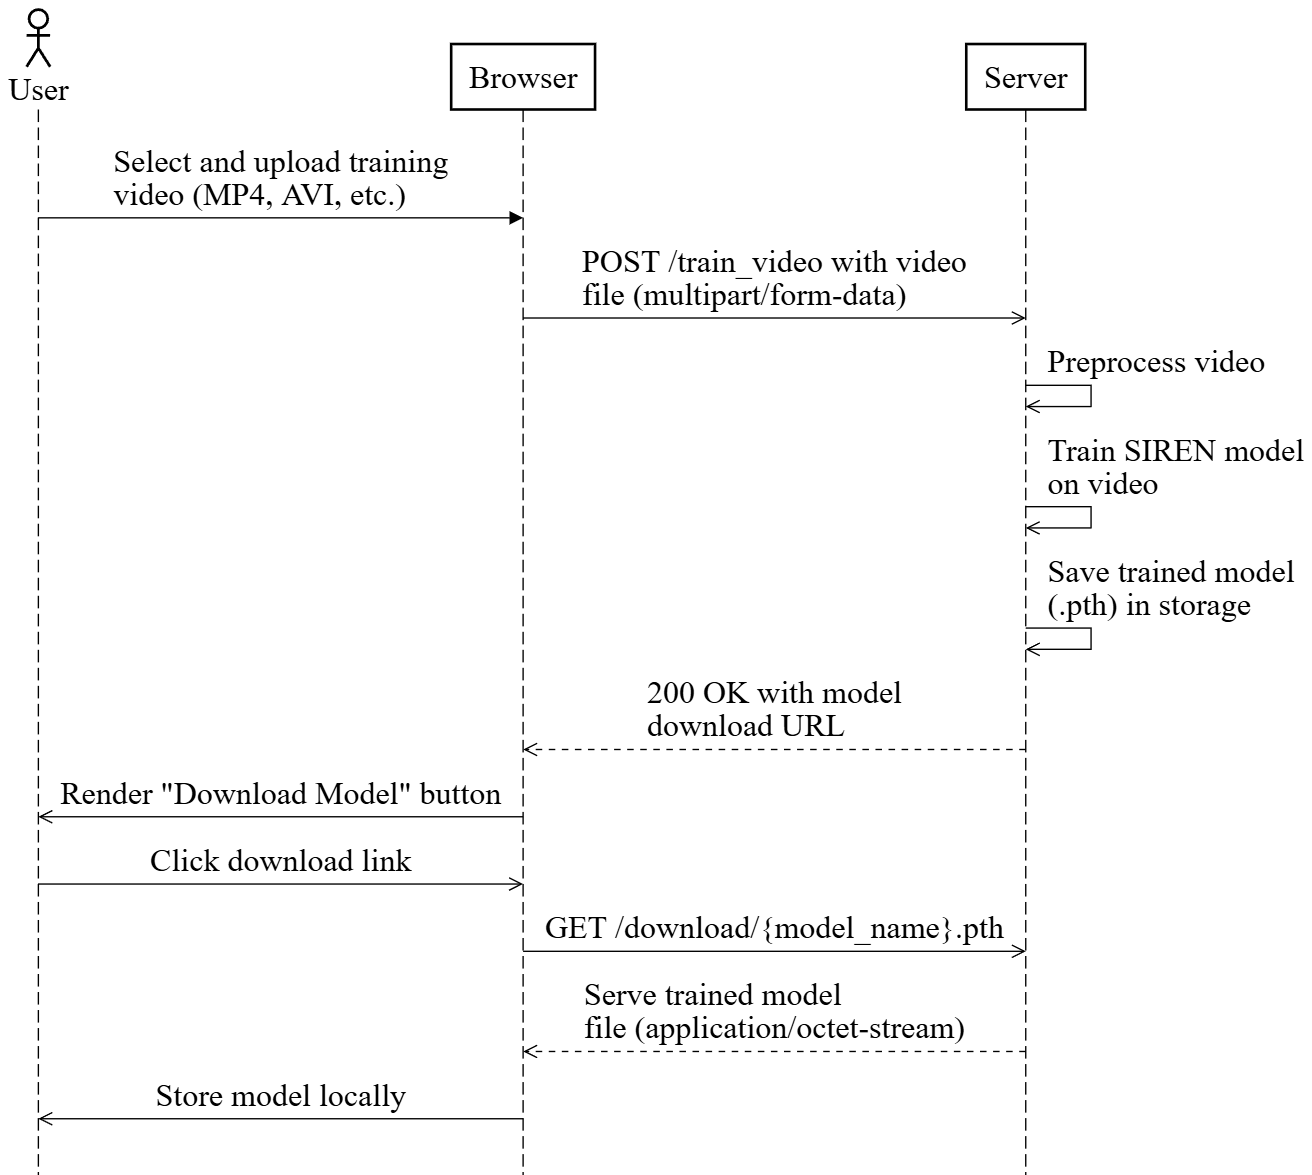
\includegraphics[width=\linewidth]{assets/website/training_seq.png}
    \caption{Sequence Diagram for Training the Model}
    \label{fig:training-seq}
\end{figure}
\autoref{fig:training-seq} illustrates the sequence of steps involved in the training of the model. It begins when the user selects and uploads a training video through the browser. The browser sends the video file to the server, which then preprocesses the video and trains the \gls{siren} model on it. Once the model is trained, it is saved and a download URL is provided back to the user through the browser. The user can then download the trained model.

\begin{figure}[H]
    \centering
    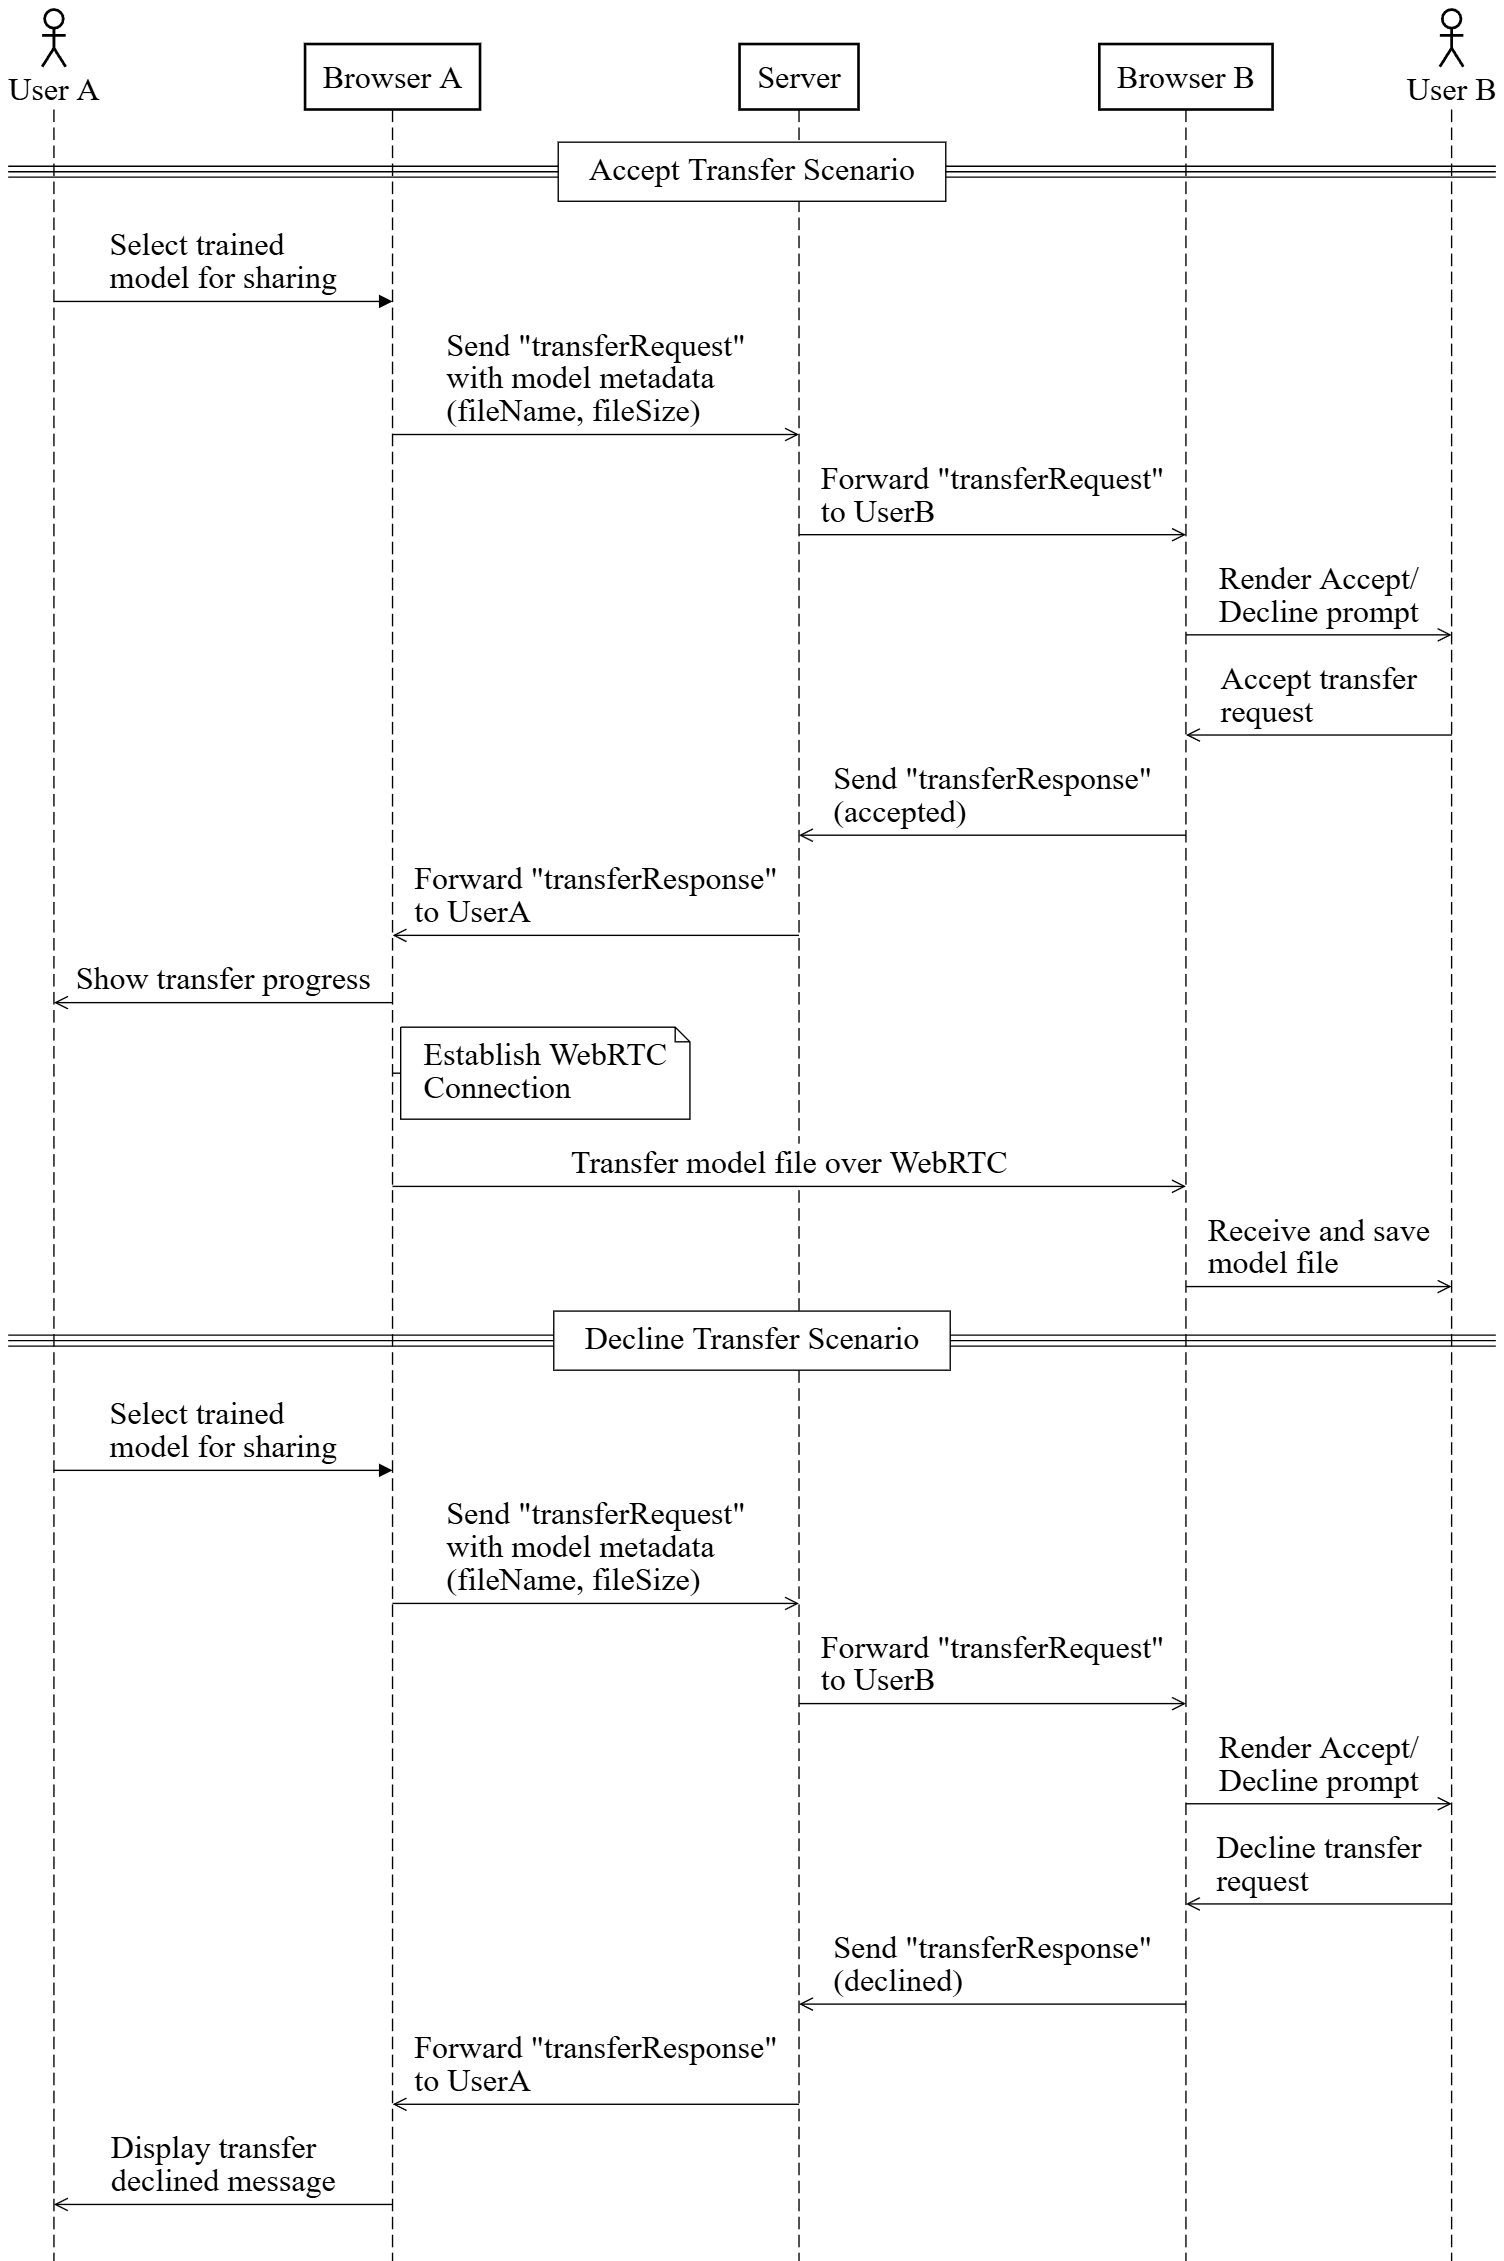
\includegraphics[width=\linewidth]{assets/website/transfer_seq.png}
    \caption{Sequence Diagram for the File Transfer}
    \label{fig:transfer-seq}
\end{figure}
\autoref{fig:transfer-seq} shows the process of transferring the trained model from one user to another. The first user selects a model for sharing, and the browser sends a transfer request to the server, including the model's metadata. The server forwards the request to the second user's browser, which prompts them to accept or decline the transfer. If accepted, the model file is transferred over a \gls{webrtc} connection; if declined, the first user is notified. This process includes scenarios for both accepting and declining the transfer.

\begin{figure}[H]
    \centering
    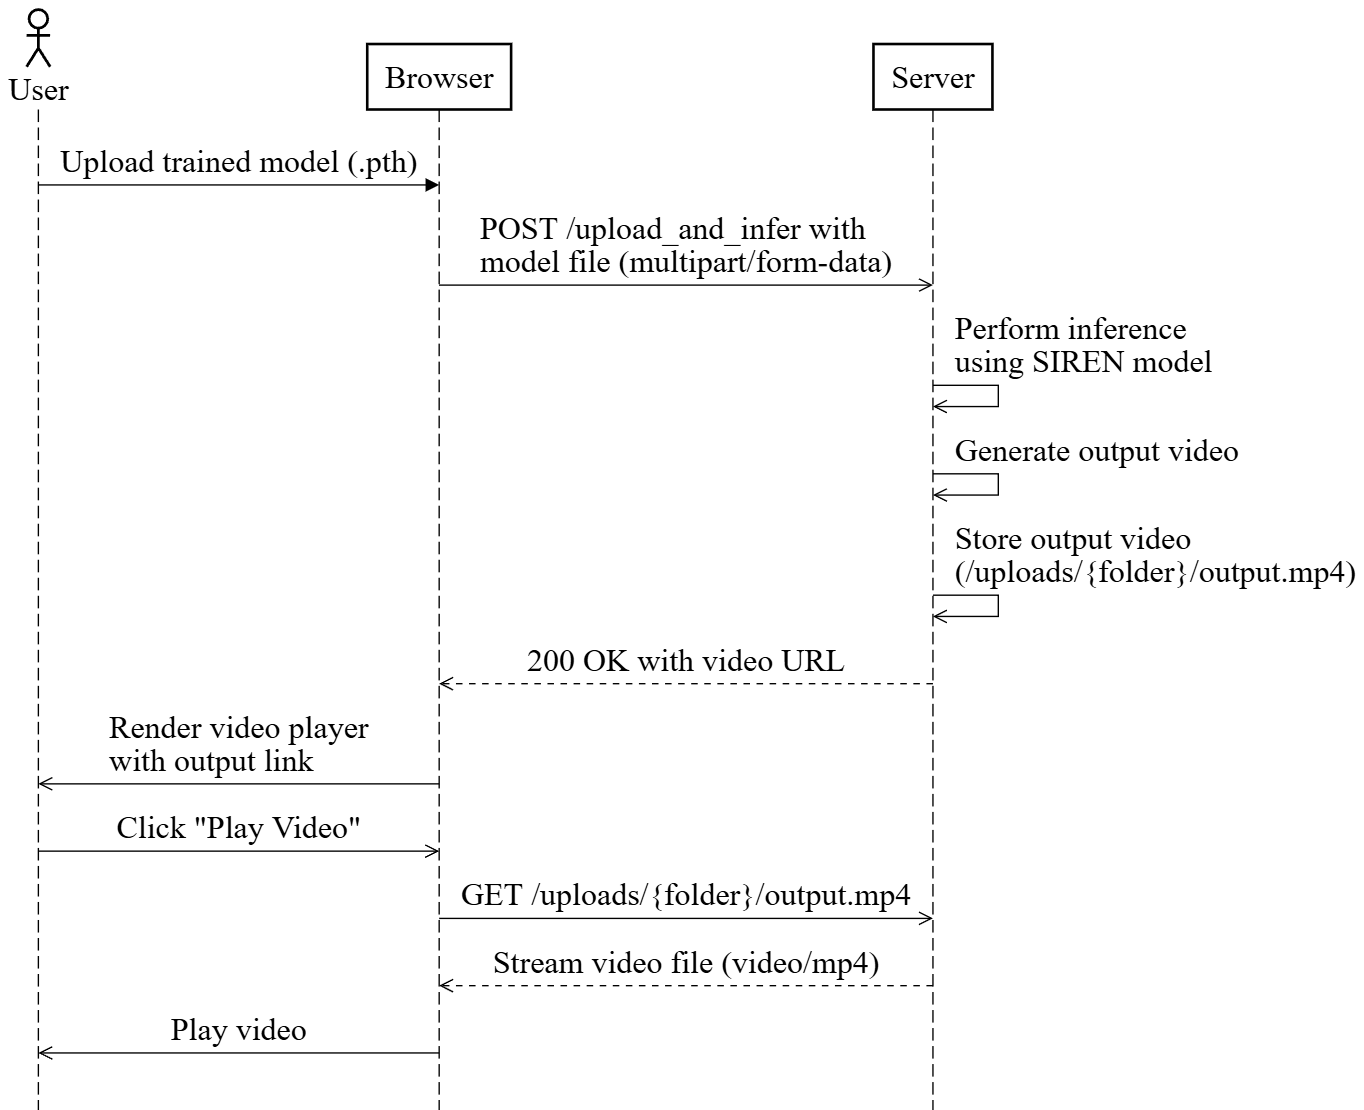
\includegraphics[width=\linewidth]{assets/website/inference_seq.png}
    \caption{Sequence Diagram for Inferencing the Model}
    \label{fig:inference-seq}
\end{figure}
\autoref{fig:inference-seq} shows the process where the user uploads a trained model file to the server for inference. The server inferences the trained \gls{siren} model, generates the output video, and stores it. The server then sends the URL of the output video back to the browser, where the user can view the video player and click ``Play Video" to stream the video from the server.

\subsubsection{Usecase Diagram}
\begin{figure}[H]
    \centering
    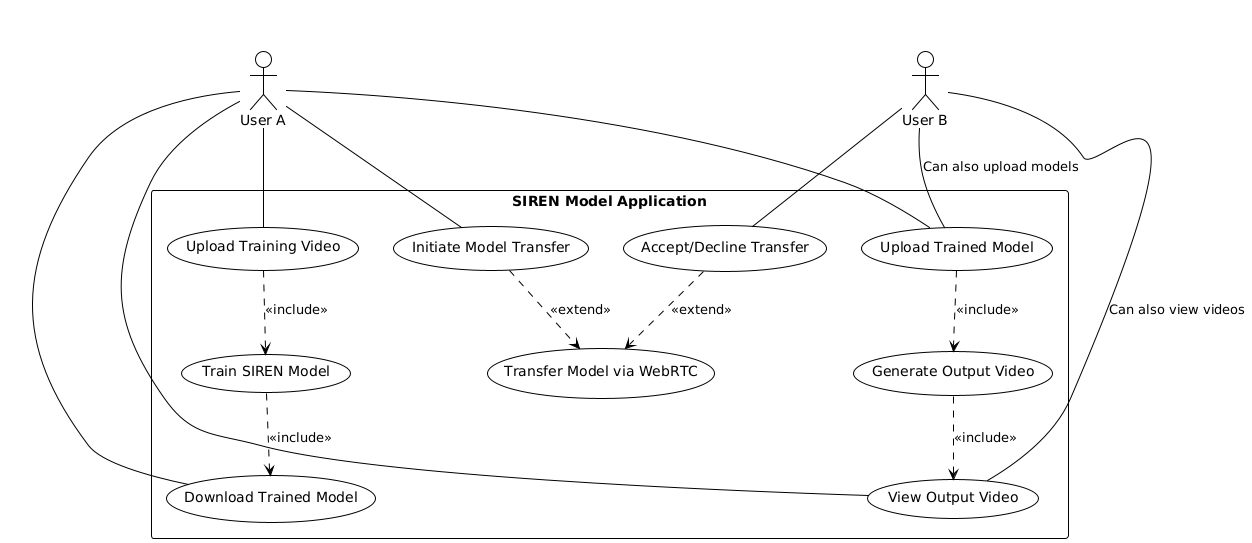
\includegraphics[width=\linewidth]{assets/website/usecase.png}
    \caption{Usecase Diagram}
    \label{fig:usecase}
\end{figure}
\autoref{fig:usecase} illustrates the use case diagram for the \gls{siren} model application. It defines the interactions between two actors, User A and User B, with various use cases related to model training, inference, and file transfer.

The diagram is divided into three primary areas:

\begin{itemize}
    \item \textbf{Model Training Related Use Cases:} This includes uploading the training video, training the \gls{siren} model, and downloading the trained model.
    \item \textbf{Model Inference Related Use Cases:} This section involves uploading the trained model, generating the output video, and viewing the output video.
    \item \textbf{File Transfer Related Use Cases:} This area includes initiating the model transfer, accepting or declining the transfer, and transferring the model via \gls{webrtc}.
\end{itemize}
\pagebreak 


\section{\MakeUppercase{Results and Analysis}}
This section covers the results and analysis of the models, including loss curves, audio analysis, comparisons with traditional codecs, and the effects of quantization.

\subsection{Teacher Model Loss Curves}

\begin{figure}[H]
    \centering
    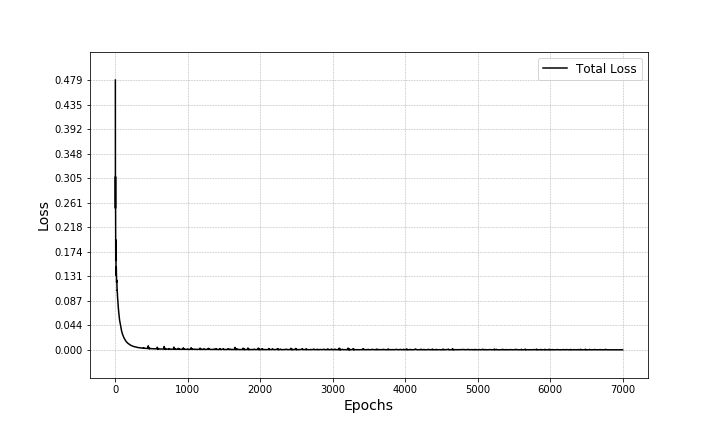
\includegraphics[height=0.6\linewidth]{assets/audio_video_loss_curves/video1_loss.png}
    \caption{Teacher Model Training Loss Curve for Video 1}
    \label{fig:video-loss-curve-1}
\end{figure}

\begin{figure}[H]
    \centering
    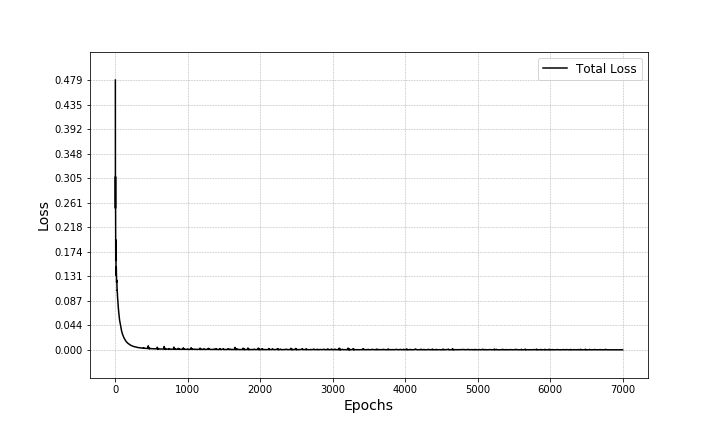
\includegraphics[height=0.6\linewidth]{assets/audio_video_loss_curves/video1_loss.png}
    \caption{Teacher Model Training Loss Curve for Video 2}
    \label{fig:video-loss-curve-2}
\end{figure}

\begin{figure}[H]
    \centering
    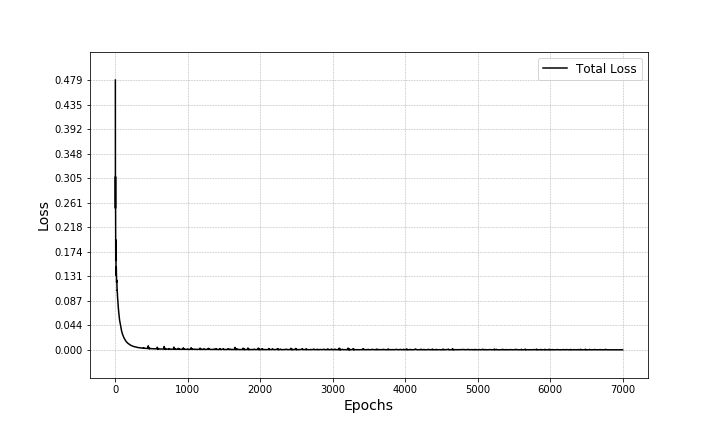
\includegraphics[height=0.6\linewidth]{assets/audio_video_loss_curves/video1_loss.png}
    \caption{Teacher Model Training Loss Curve for Video 3}
    \label{fig:video-loss-curve-3}
\end{figure}

\begin{figure}[H]
    \centering
    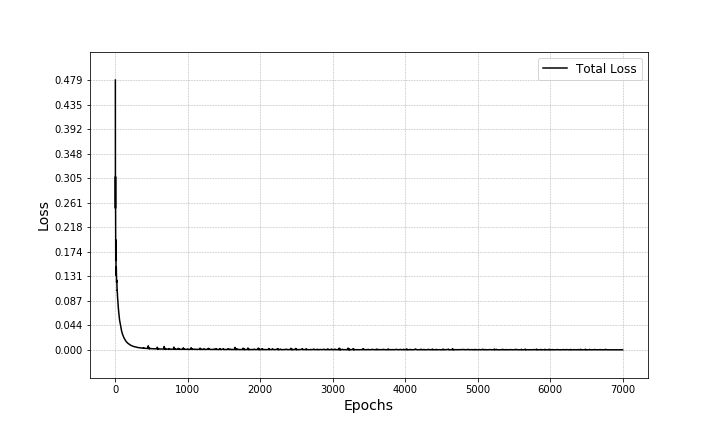
\includegraphics[height=0.6\linewidth]{assets/audio_video_loss_curves/video1_loss.png}
    \caption{Teacher Model Training Loss Curve for Video 4}
    \label{fig:video-loss-curve-4}
\end{figure}

\begin{figure}[H]
    \centering
    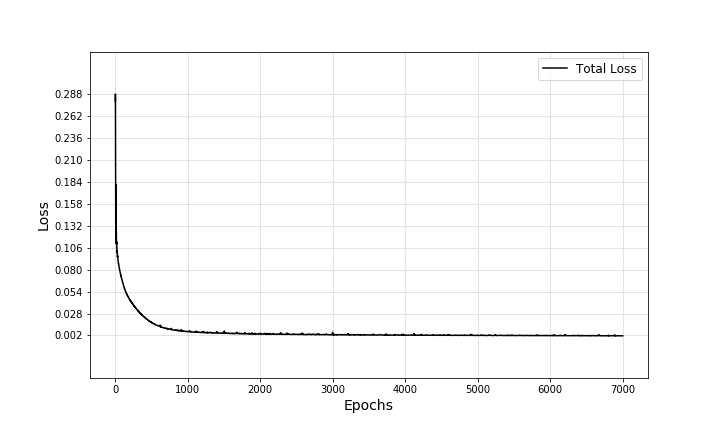
\includegraphics[height=0.6\linewidth]{assets/audio_video_loss_curves/video5_loss.png}
    \caption{Teacher Model Training Loss Curve for Video 5}
    \label{fig:video-loss-curve-5}
\end{figure}


The loss values for the model start at a low level and show a very steep decline, approaching nearly zero around epoch 500. After this point, the rate of decline in the loss slows down almost being linear. Although the loss value approaches zero, training continues beyond this point. This is because even though there were only minute improvements in the loss function the performance metrics such as \gls{psnr}, \gls{ssim}, \gls{lpips}, \gls{lsd} were improving. The continued training ensured that these evaluation metrics were optimized, further enhancing the quality of the video representation model.

\subsection{Student Model Loss Curves}

\begin{figure}[H]
    \centering
    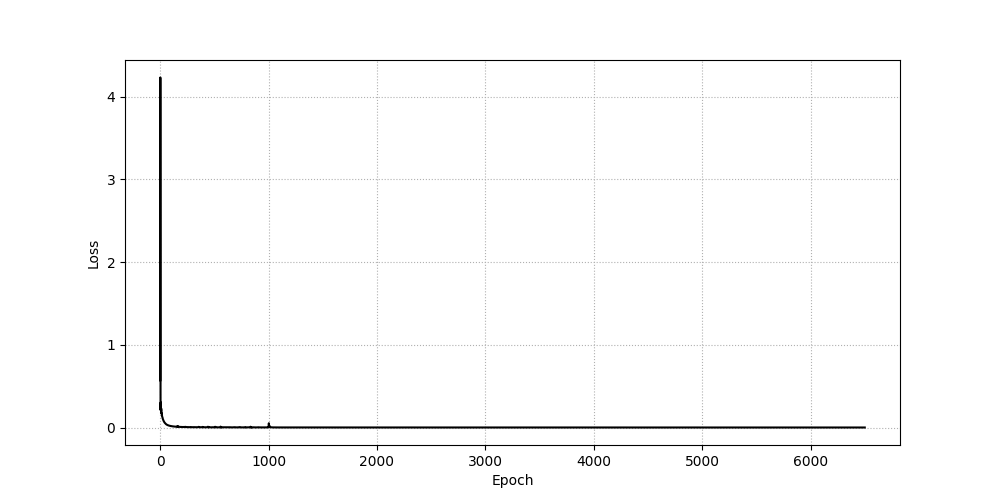
\includegraphics[width=1\linewidth,height=0.6\linewidth]{assets/quantization/student_vvsa_loss_curve.png}
    \caption{Student Model Training Loss Curve of Video 1}
    \label{fig:student-video-loss-curve-1}
\end{figure}

\begin{figure}[H]
    \centering
    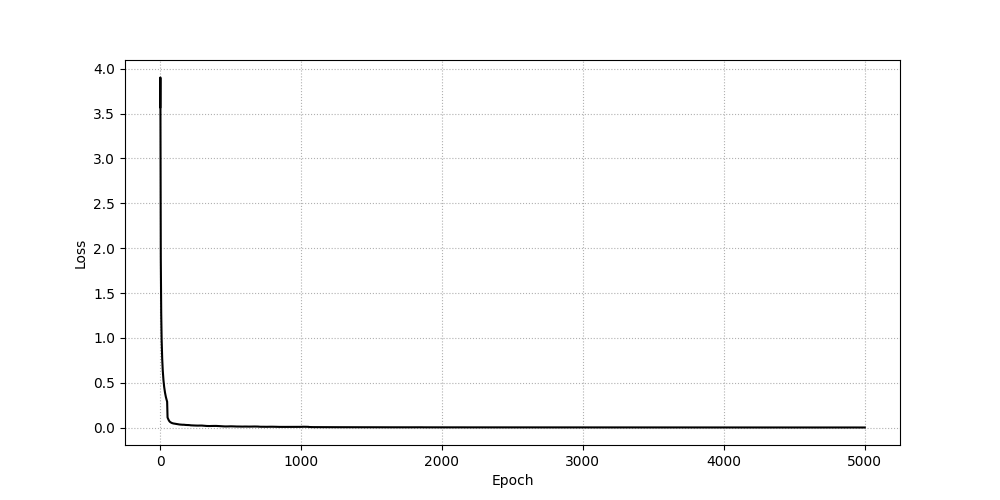
\includegraphics[width=1\linewidth,height=0.6\linewidth]{assets/quantization/student_rick_loss_curve.png}
    \caption{Student Model Training Loss Curve of Video 3}
    \label{fig:student-video-loss-curve-3}
\end{figure}

Initially, the loss begins at a relatively high value, with a sharp and rapid decline within the first few hundred epochs, indicating significant progress in optimizing the model. Within epoch 200, the loss value stabilizes and approaches nearly zero, with further reductions becoming progressively smaller and almost linear in trend. Although the improvements in the loss function become minimal after this point, training continues in the same manner as for the teacher models.

\subsection{FFT and Spectrogram Analysis of Audio Content Across Videos}
This section provides a visual analysis of the fidelity of the audio predictions by comparing the ground truth and predicted signals in both the time and frequency domains.

\begin{figure}[H]
    \centering
    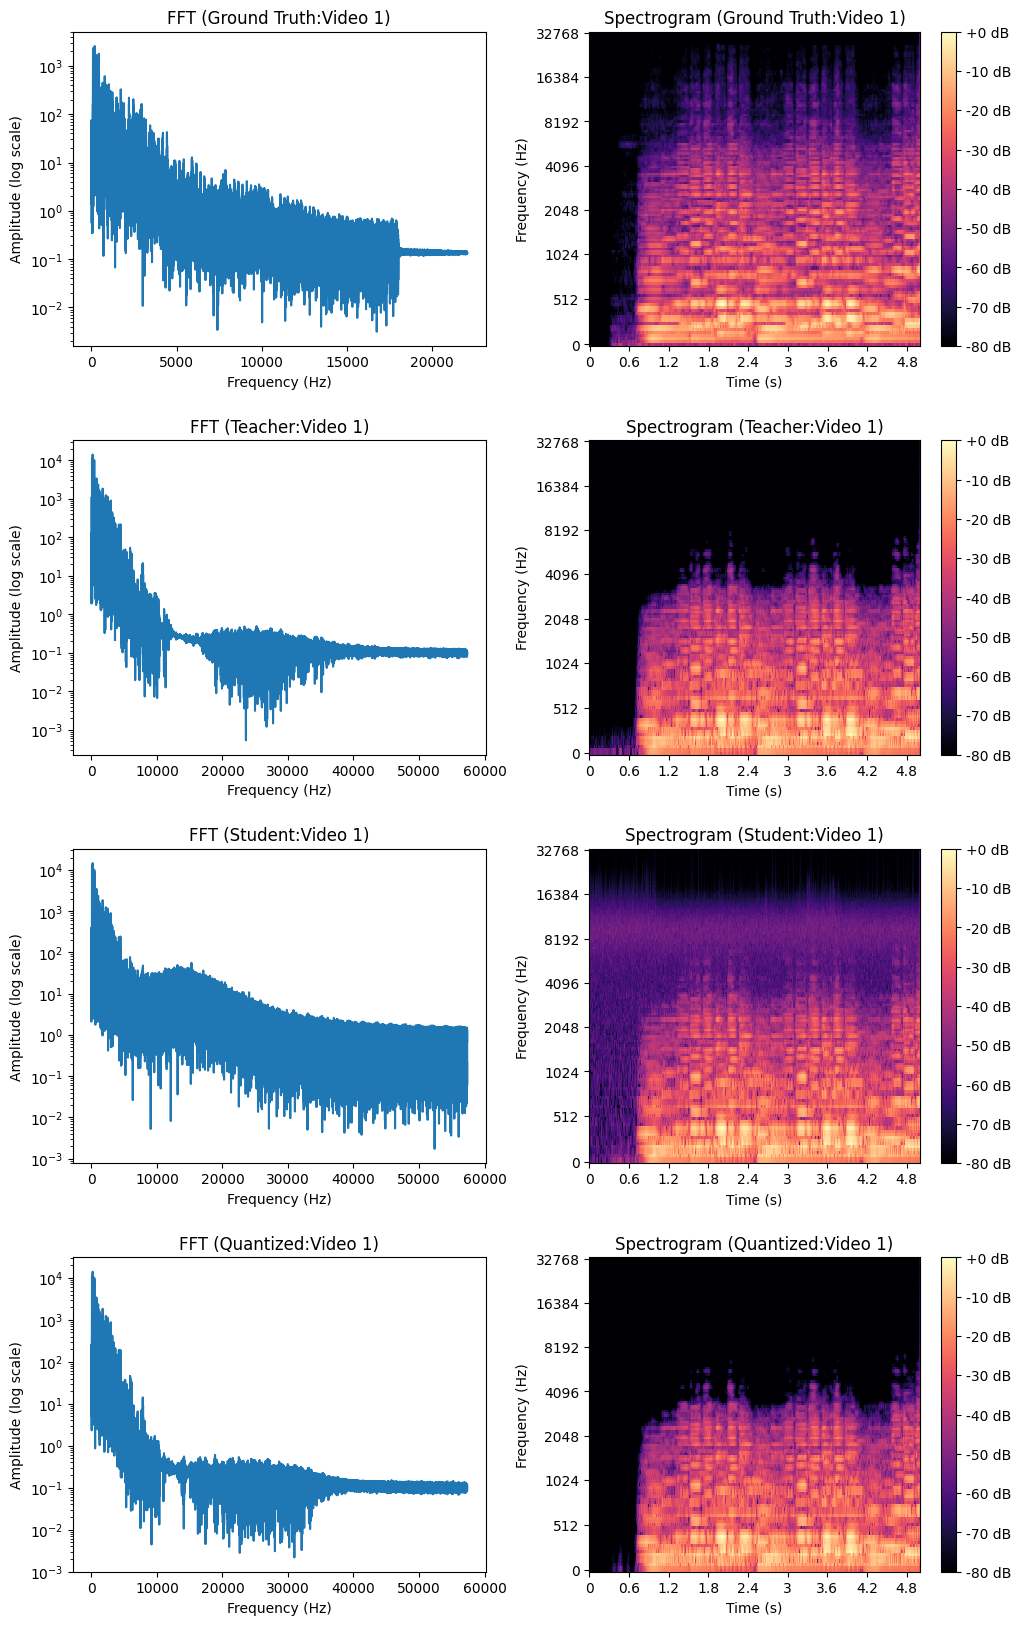
\includegraphics[width=0.8\linewidth]{assets/quantization/fft_spectrogram_Video1.png}
    \caption{FFT and Spectrogram Analysis of Audio Content in Video 1}
    \label{fig:fft-spec-v1}
\end{figure}

\begin{figure}[H]
    \centering
    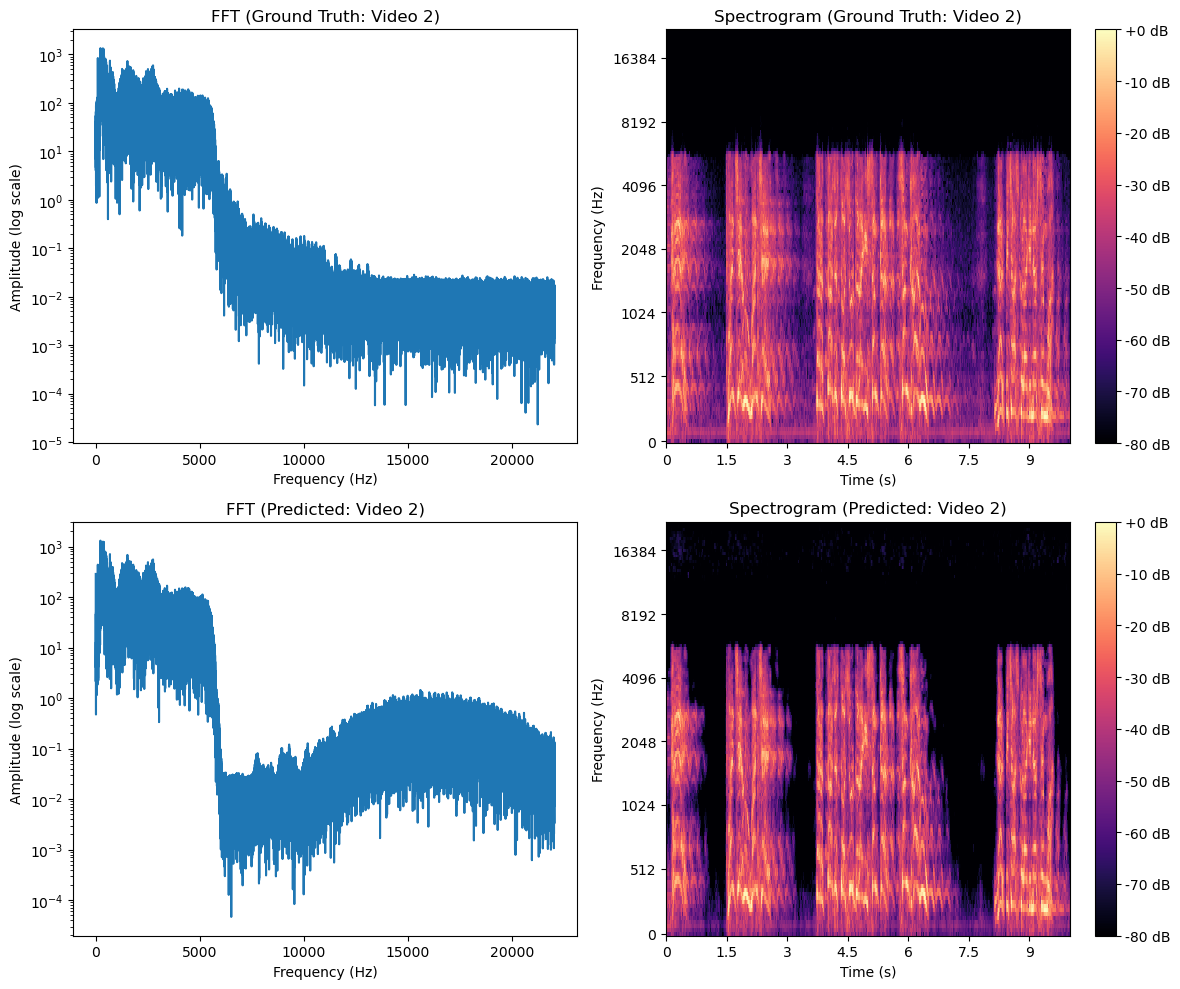
\includegraphics[width=0.8\linewidth]{assets/audio_video_analysis/Video_2_analysis.png}
    \caption{FFT and Spectrogram Analysis of Audio Content in Video 2}
    \label{fig:fft-spec-v2}
\end{figure}

\begin{figure}[H]
    \centering
    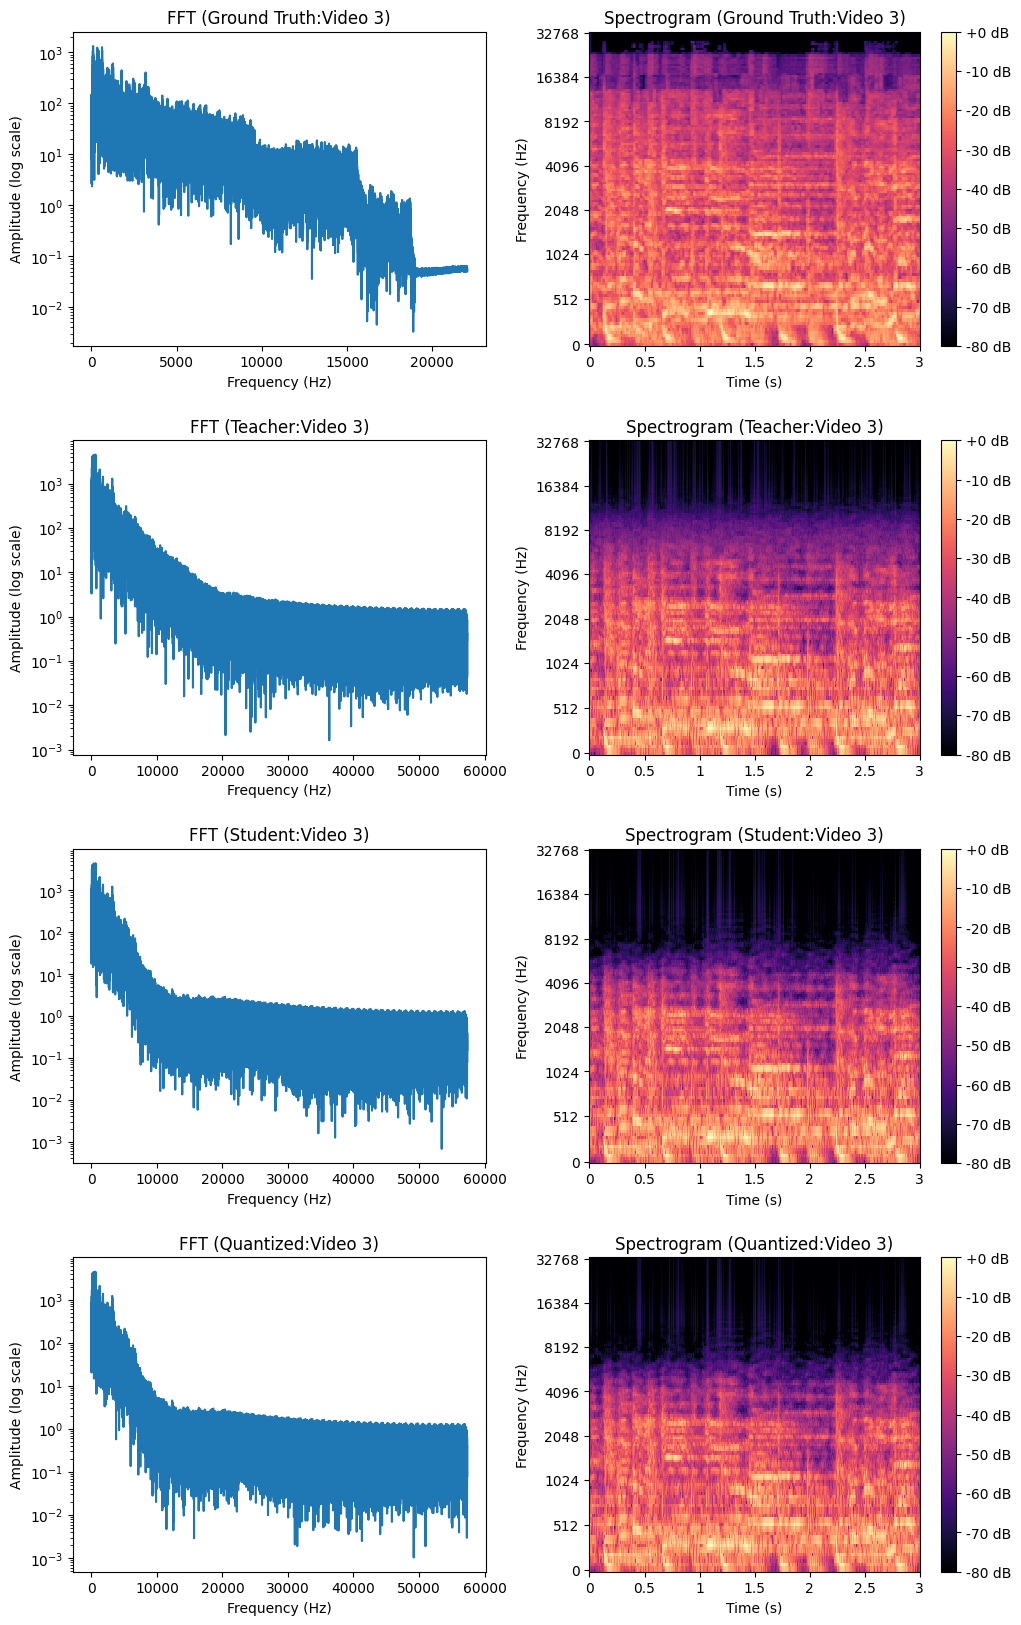
\includegraphics[width=0.7\linewidth]{assets/quantization/fft_spectrogram_Video3.png}
    \caption{FFT and Spectrogram Analysis of Audio Content in Video 3}
    \label{fig:fft-spec-v3}
\end{figure}

\begin{figure}[H]
    \centering
    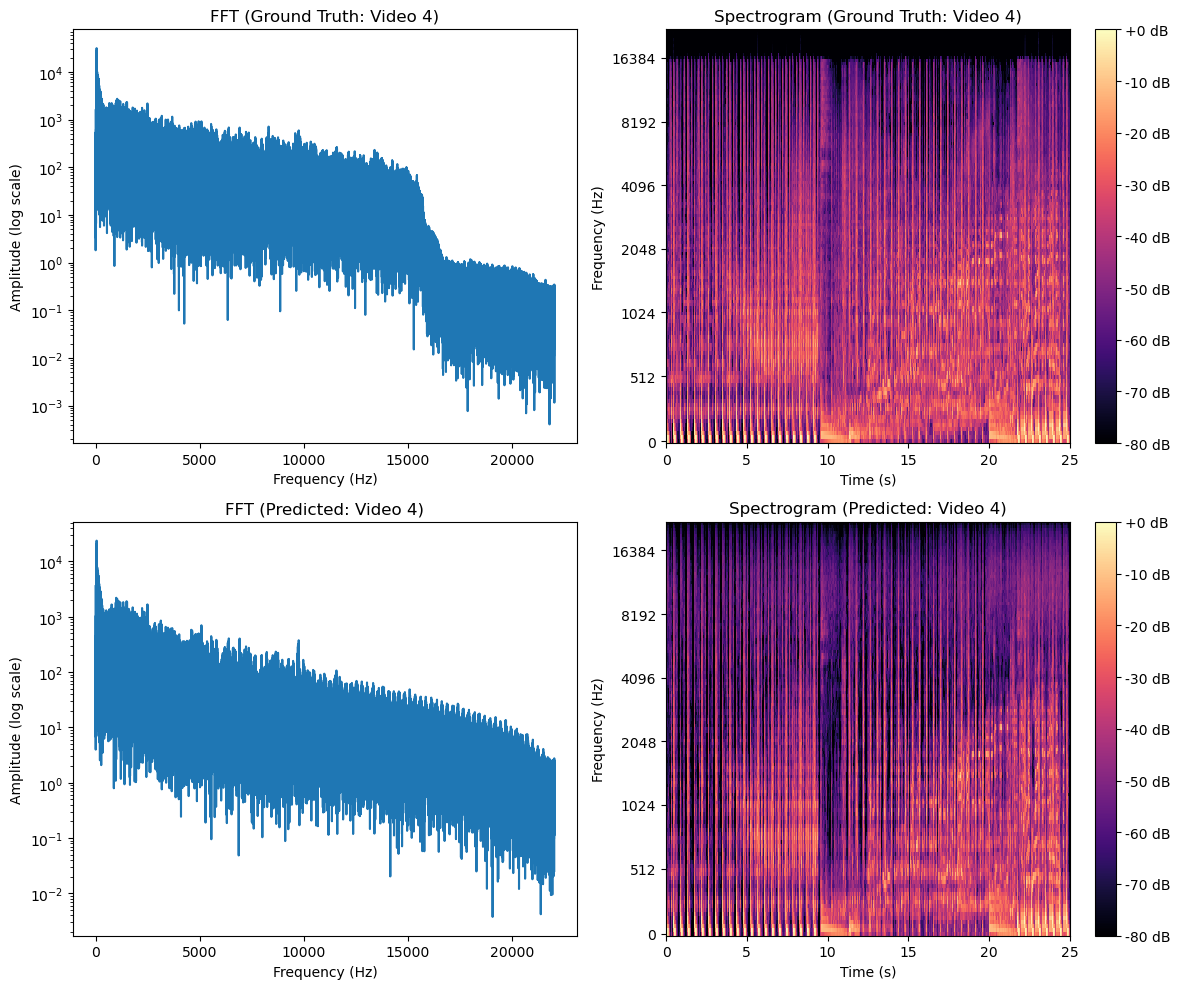
\includegraphics[width=0.8\linewidth]{assets/audio_video_analysis/Video_4_analysis.png}
    \caption{FFT and Spectrogram Analysis of Audio Content in Video 4}
    \label{fig:fft-spec-v4}
\end{figure}

\begin{figure}[H]
    \centering
    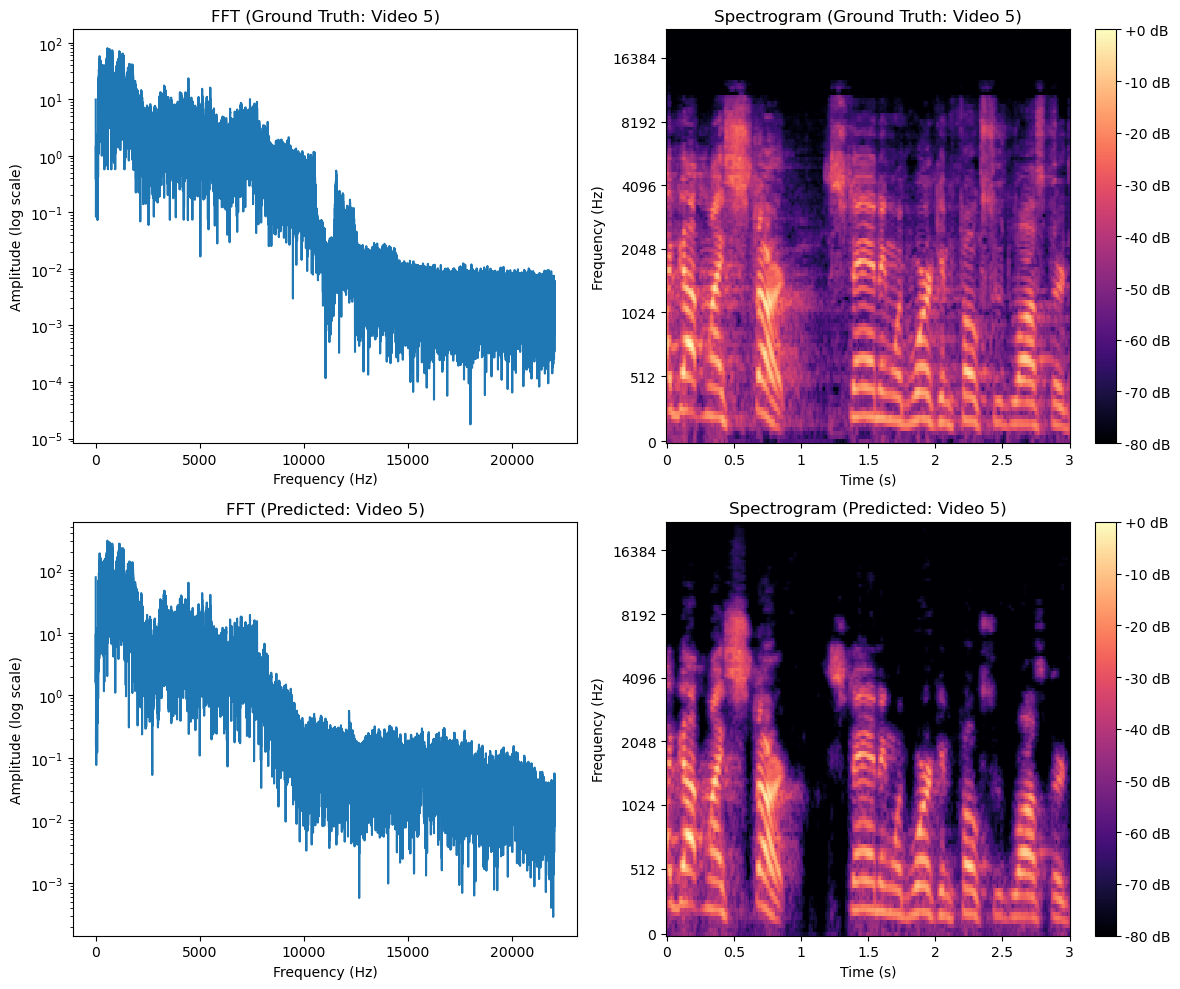
\includegraphics[width=0.8\linewidth]{assets/audio_video_analysis/Video_5_analysis.png}
    \caption{FFT and Spectrogram Analysis of Audio Content in Video 5}
    \label{fig:fft-spec-v5}
\end{figure}

The \gls{fft} and spectrogram plots of the audio content in the inferenced videos closely resemble the ground truth plots across all videos. The model successfully recreates the audio signals with various frequency components, although slight deviations are observed in the FFT plots. However, the spectrograms remain almost identical across all videos, demonstrating the model's ability to capture the temporal structure of the audio. 

In the spectrogram of Video 2 and Video 5, a slight loss of signal is noticable, which can be attributed to the application of the noise reduction algorithm. This algorithm appears to have mistakenly identified some parts of the signal as noise and removed them, leading to this minor discrepancy.


\subsection{Comparision with Traditional Codecs}
    \subsubsection{Performance Metrics of Teacher Model}
    \begin{table}[H]
        \centering
        \caption{Video Metrics of Teacher Model}
        \label{table:video-metric-teacher}
        \begin{tabular}{|c|c|c|c|c|c|c|}
        \hline
        \multirow{2}{*}{\textbf{Video}} & \textbf{PSNR} & \multirow{2}{*}{\textbf{LPIPS}} & \multirow{2}{*}{\textbf{SSIM}} & \textbf{Original} & \textbf{Model Size} & \textbf{Compression} \\
        & \textbf{(dB)} &  &  & \textbf{Size (KiB)} & \textbf{(KiB)} & \textbf{Ratio} \\
        \hline
        Video 1 & 42.69 & 0.05 & 0.98 & 1972 & \multirow{5}{*}{9260} & 0.21 \\
        \cline{1-5} \cline{7-7}
        Video 2 & 35.08 & 0.17 & 0.92 & 5462 &  & 0.58 \\
        \cline{1-5} \cline{7-6}
        Video 3 & 21.88 & 0.39 & 0.67 & 6235 &  & 0.67 \\
        \cline{1-5} \cline{7-7}
        Video 4 & 26.89 & 0.41 & 0.72 & 14018 &  & 1.50 \\
        \cline{1-5} \cline{7-7}
        Video 5 & 32.88 & 0.21 & 0.92 & 12781 &  & 1.37 \\
        \hline
        \end{tabular}
    \end{table}
    
    \begin{table}[H]
        \centering
        \caption{Audio Metrics of Teacher Model}
        \label{table:audio-metric-teacher}
        \begin{tabular}{|c|c|c|c|}
        \hline
        \multirow{2}{*}{\textbf{Video}} & \textbf{PSNR} & \textbf{LSD} & \multirow{2}{*}{\textbf{ViSQOL}}\\
        & \textbf{(dB)} & \textbf{(dB)} &  \\
        \hline
        Video 1 & 57.57 & 4.50 & 3.54 \\
        \hline
        Video 2 & 57.09 & 4.28 & 3.35 \\
        \hline
        Video 3 & 62.50 & 7.60 & 4.51 \\
        \hline
        Video 4 & 64.33 & 8.15 & 3.58 \\
        \hline
        Video 5 & 46.60 & 6.89 & 2.66 \\
        \hline
        \end{tabular}
    \end{table}

    \autoref{table:video-metric-teacher} presents the video metrics of the teacher model, showing the \gls{psnr}, \gls{lpips}, \gls{ssim}, original video size, model size, and compression ratio for five different videos. The \gls{psnr} values range from 21.88 dB to 42.69 dB, indicating a notable variation in video quality. Video 1 achieves the highest \gls{psnr} at 42.69 dB, demonstrating superior quality compared to the other videos. In contrast, Video 3 has the lowest \gls{psnr} of 21.88 dB, reflecting a lower-quality reconstruction. The \gls{ssim} values remain high, suggesting that the model preserves structural details well across all videos, with values ranging from 0.67 to 0.98. The compression ratios vary from 0.21 for Video 1 to 1.50 for Video 4, showing how compression affects the model's storage efficiency and output size.

    \autoref{table:audio-metric-teacher} shows the audio metrics for the teacher model, including \gls{psnr}, \gls{lsd}, and \gls{visqol} scores for each video. The \gls{psnr} values indicate high fidelity, with Video 3 achieving the highest \gls{psnr} at 62.50 dB, while Video 5 has the lowest at 46.60 dB. The \gls{lsd} values indicate the level of distortion, with Video 1 having the lowest value of 4.50 dB, signifying better quality. The \gls{visqol} scores, which evaluate perceptual quality, show consistency across most videos, with Video 3 achieving the highest score of 4.51. Overall, the audio metrics indicate that the teacher model performs well, but there is a slight decline in performance for Video 5, particularly in terms of \gls{psnr} and \gls{visqol}.


\subsubsection{Performance Metrics of Student Model with Quantization}
    Quantization impacts the quality of reconstructed images and audio, as measured by PSNR, SSIM and LSD. It also reduces file size. The following table shows the performance metrics for student model before and after quantization to 16-bit.

    \begin{table}[H]
        \centering
        \caption{Metrics Before and After Quantization of Student Model for Video 1}
        \label{tab:metrics-quantization-video-1}
        \begin{tabular}{|c|c|c|c|}
            \hline
            \multirow{2}{*}{\textbf{Metrics}} & \multicolumn{2}{c|}{\textbf{Value}} \\ \cline{2-3}
            & \textbf{Student Model} & \textbf{16-bit Quantization} \\ \hline
            \textbf{PSNR(Frames)(dB)} & 35.5525 & 35.3520 \\ \hline
            \textbf{SSIM} & 0.9194 & 0.9189 \\ \hline
            \textbf{LPIPS} & 0.0794 & 0.0848\\ \hline
            \textbf{PSNR(Audio)(dB)} & 18.7929 & 18.8487  \\ \hline
            \textbf{LSD(dB)} & 4.5930 & 4.8484 \\ \hline
            % \textbf{VISQOL} & & \\ \hline
            \textbf{SQNR(dB)} & - & 39.214 \gls{db} \\ \hline
            \textbf{File Size(MiB)} & 4.96 & 2.48 \\ \hline
            \textbf{Compression Ratio} & 0.38 & 0.77 \\ \hline
        \end{tabular}
    \end{table}

    The results from the \autoref{tab:metrics-quantization-video-1} demonstrate the effect of quantization on both video and audio quality for Video 1. A significant reduction in file size is observed, dropping from 4.96 \gls{mib} to 2.48 \gls{mib}, a 50\% reduction. Despite this compression, the quality metrics indicate only minor degradation. The PSNR for the video frames decreased slightly from 35.5525 \gls{db} to 35.3520 \gls{db}, showing that the overall visual quality remains almost unchanged post-quantization. Similarly, the \gls{ssim} metric, which measures structural similarity, experienced a marginal decrease from 0.9194 to 0.9189, indicating that the structural integrity of the video is nearly preserved.

    The \gls{sqnr} value at 39.214 \gls{db} provides a robust measure of the quantization noise introduced during the compression process. This relatively high value suggests that the noise is effectively controlled, ensuring that the perceived quality remains satisfactory. The audio metrics show a slight improvement, with the \gls{psnr} increasing from 18.7929 \gls{db} to 18.8487 \gls{db}, suggesting that the audio quality benefits slightly from the quantization process. However, the \gls{lsd} value increased from 4.5930 \gls{db} to 4.8484 \gls{db}, indicating a slight degradation in the audio frequency spectrum. Nevertheless, this change is minimal and does not significantly affect the overall audio experience. The overall file size reduction highlights the efficiency of quantization in compressing both video and audio, with manageable trade-offs in quality.

    \begin{table}[H]
        \centering
        \caption{Metrics Before and After Quantization of Student Model for Video 3}
        \label{tab:metrics-quantization-video-3}
        \begin{tabular}{|c|c|c|c|}
            \hline
            \multirow{2}{*}{\textbf{Metrics}} & \multicolumn{2}{c|}{\textbf{Value}} \\ \cline{2-3}
            & \textbf{Student Model} & \textbf{16-bit Quantization} \\ \hline
            \textbf{PSNR(Frames)(dB)} & 28.8588 & 28.7153 \\ \hline
            \textbf{SSIM} & 0.7579 & 0.7529 \\ \hline
            \textbf{LPIPS} & 0.4039 & 0.4126 \\ \hline
            \textbf{PSNR(Audio)(dB)} & 24.1992 & 24.1786 \\ \hline
            \textbf{LSD(dB)} & 10.7038 & 10.6928 \\ \hline
            \textbf{File Size(MiB)} & 4.96 & 2.48 \\ \hline
            \textbf{Compression Ratio} & 1.22 & 2.45\\ \hline
        \end{tabular}
    \end{table}

    The results in \autoref{tab:metrics-quantization-video-3} show the impact of quantization on Video 2. As with Video 1, the file size is reduced by 50\%, from 4.96 \gls{mib} to 2.48 \gls{mib}, demonstrating the effectiveness of quantization in compressing the video. The \gls{psnr} for video frames decreased slightly from 28.8588 \gls{db} to 28.7153 \gls{db}, indicating minimal visual quality degradation, and the \gls{ssim} dropped marginally from 0.7579 to 0.7529, suggesting that the structural integrity is similarly well-preserved.

    For the audio, the \gls{psnr} showed a negligible change, from 24.1992 \gls{db} to 24.1786 \gls{db}, and the \gls{lsd} remained almost the same, moving from 10.7038 \gls{db} to 10.6928 \gls{db}, further confirming that the audio quality remains stable after quantization. Overall, the results are consistent with those observed in Video 1, indicating a good balance between file size reduction and quality retention.


    \subsubsection{Performance Metrics of Traditional Codecs}

    % Video Metrics Table
    \begin{table}[H]
        \centering
        \caption{Metrics for Video Content of Video 1}
        \label{table:vid-met-1}
        \begin{tabular}{|c|c|c|c|c|c|c|c|}
        \hline
        \multicolumn{8}{|c|}{\textbf{Video 1 (1972 KiB)}} \\ \hline
        \multirow{2}{*}{\textbf{Codec}} & \multirow{2}{*}{\textbf{CRF}} & \textbf{Bitrate} & \textbf{PSNR} & \textbf{SSIM} & \textbf{LPIPS} & \textbf{File Size} & \textbf{Compression} \\ 
        &  & \textbf{(kbps)} & \textbf{(dB)} &  &  & \textbf{(KiB)} & \textbf{Ratio} \\ \hline
        \multirow{3}{*}{H.264/MP3} & 1  & 320 & 61.60 & 0.99 & 0.004 & 429.64  & 4.59 \\ \cline{2-8} 
                                & 23 & 192 & 47.24 & 0.99 & 0.005 & 178.59  & 11.04 \\ \cline{2-8} 
                                & 51 & 64  & 32.00 & 0.83 & 0.23 & 44.28   & 44.52 \\ \hline
        \multirow{3}{*}{H.265/MP3} & 1  & 320 & 59.53 & 0.99 & 0.004 & 378.32  & 5.21 \\ \cline{2-8} 
                                & 28 & 192 & 45.32 & 0.98 & 0.02 & 154.51  & 12.76 \\ \cline{2-8} 
                                & 51 & 64  & 33.37 & 0.85 & 0.21 & 45.70   & 43.14 \\ \hline
        \end{tabular}
    \end{table}

    \begin{table}[H]
        \centering
        \caption{Metrics for Audio content of Video 1}
        \label{table:aud-met-1}
        \begin{tabular}{|c|c|c|c|c|}
        \hline
        \textbf{Codec} & \textbf{Bitrate (kbps)} & \textbf{PSNR (dB)} & \textbf{LSD} & \textbf{VISQOL} \\ \hline
        \multirow{3}{*}{MP3} & 64  & 35.34 & 1.97 & 4.66 \\ \cline{2-5} 
                                   & 192 & 43.28 & 0.42 & 4.73 \\ \cline{2-5} 
                                   & 320 & 64.78 & 0.10 & 4.73 \\ \hline
        \end{tabular}
    \end{table}
    
    

    \begin{table}[H]
        \centering
        \caption{Metrics for Video Content of Video 2}
        \label{table:vid-met-2}
        \begin{tabular}{|c|c|c|c|c|c|c|c|}
        \hline
        \multicolumn{8}{|c|}{\textbf{Video 2 (5462 KiB)}} \\ \hline
        \multirow{2}{*}{\textbf{Codec}} & \multirow{2}{*}{\textbf{CRF}} & \textbf{Bitrate} & \textbf{PSNR} & \textbf{SSIM} & \textbf{LPIPS} & \textbf{File Size} & \textbf{Compression} \\ 
        &  & \textbf{(kbps)} & \textbf{(dB)} &  &  & \textbf{(KiB)} & \textbf{Ratio} \\ \hline
        \multirow{3}{*}{H.264/MP3} & 1  & 320 & 59.70 & 0.99 & 0.003 & 632 & 2.67 \\ \cline{2-8} 
                                & 23 & 192 & 44.94 & 0.98 & 0.005 & 190 & 8.87 \\ \cline{2-8} 
                                & 51 & 64  & 27.75 & 0.78 & 0.22 & 12  & 140.50 \\ \hline
        \multirow{3}{*}{H.265/MP3} & 1  & 320 & 52.13 & 0.99 & 0.004 & 434 & 3.88 \\ \cline{2-8} 
                                & 28 & 192 & 41.57 & 0.97 & 0.01 & 128 & 13.17 \\ \cline{2-8} 
                                & 51 & 64  & 27.83 & 0.76 & 0.29 & 14  & 120.40 \\ \hline
        \end{tabular}
    \end{table}
    

    \begin{table}[H]
        \centering
        \caption{Metrics for Audio content of Video 2}
        \label{table:aud-met-2}
        \begin{tabular}{|c|c|c|c|c|}
        \hline
        \textbf{Codec} & \textbf{Bitrate (kbps)} & \textbf{PSNR (dB)} & \textbf{LSD} & \textbf{VISQOL} \\ \hline
        \multirow{3}{*}{MP3} & 64  & 38.99 & 0.73 & 4.72 \\ \cline{2-5} 
                                   & 192 & 45.82 & 0.04 & 4.73 \\ \cline{2-5} 
                                   & 320 & 86.68 & 0.01 & 4.73 \\ \hline
        \end{tabular}
    \end{table}
    




    \begin{table}[H]
        \centering
        \caption{Metrics for Video Content of Video 3}
        \label{table:vid-met-3}
        \begin{tabular}{|c|c|c|c|c|c|c|c|}
        \hline
        \multicolumn{8}{|c|}{\textbf{Video 3 (6235 KiB)}} \\ \hline
        \multirow{2}{*}{\textbf{Codec}} & \multirow{2}{*}{\textbf{CRF}} & \textbf{Bitrate} & \textbf{PSNR} & \textbf{SSIM} & \textbf{LPIPS} & \textbf{File Size} & \textbf{Compression} \\ 
        &  & \textbf{(kbps)} & \textbf{(dB)} &  &  & \textbf{(KiB)} & \textbf{Ratio} \\ \hline
        \multirow{3}{*}{H.264/MP3} & 1  & 320 & 58.39 & 0.98 & 0.16 & 1218.82 & 5.12 \\ \cline{2-8} 
                                   & 23 & 192 & 42.22 & 0.96 & 0.16 & 161.85  & 38.52 \\ \cline{2-8} 
                                   & 51 & 64  & 22.17 & 0.72 & 0.34 & 31.65   & 196.98 \\ \hline
        \multirow{3}{*}{H.265/MP3} & 1  & 320 & 56.07 & 0.99 & 0.16 & 861.80  & 7.23 \\ \cline{2-8} 
                                   & 28 & 192 & 40.20 & 0.96 & 0.18 & 113.02  & 55.16 \\ \cline{2-8} 
                                   & 51 & 64  & 24.16 & 0.73 & 0.35 & 31.42   & 198.39 \\ \hline
        \end{tabular}
    \end{table}
    


    \begin{table}[H]
        \centering
        \caption{Metrics for Audio content of Video 3}
        \label{table:aud-met-3}
        \begin{tabular}{|c|c|c|c|c|}
        \hline
        \textbf{Codec} & \textbf{Bitrate (kbps)} & \textbf{PSNR (dB)} & \textbf{LSD} & \textbf{VISQOL} \\ \hline
        \multirow{3}{*}{MP3} & 64  & 27.99 & 4.21 & 4.64 \\ \cline{2-5} 
                                   & 192 & 42.23 & 0.75 & 4.73 \\ \cline{2-5} 
                                   & 320 & 66.45 & 0.18 & 4.73 \\ \hline
        \end{tabular}
    \end{table}
    



    \begin{table}[H]
        \centering
        \caption{Metrics for Video Content of Video 4}
        \label{table:vid-met-4}
        \begin{tabular}{|c|c|c|c|c|c|c|c|}
        \hline
        \multicolumn{8}{|c|}{\textbf{Video 4 (14018 KiB)}} \\ \hline
        \multirow{2}{*}{\textbf{Codec}} & \multirow{2}{*}{\textbf{CRF}} & \textbf{Bitrate} & \textbf{PSNR} & \textbf{SSIM} & \textbf{LPIPS} & \textbf{File Size} & \textbf{Compression} \\ 
        &  & \textbf{(kbps)} & \textbf{(dB)} &  &  & \textbf{(KiB)} & \textbf{Ratio} \\ \hline
        \multirow{3}{*}{H.264/MP3} & 1  & 320 & 59.10 & 0.99 & 0.00 & 4225.52 & 3.32 \\ \cline{2-8} 
                                   & 23 & 192 & 41.20 & 0.98 & 0.00 & 1146.30 & 12.23 \\ \cline{2-8} 
                                   & 51 & 64  & 24.39 & 0.61 & 0.32 & 215.05  & 65.18 \\ \hline
        \multirow{3}{*}{H.265/MP3} & 1  & 320 & 57.61 & 0.99 & 0.00 & 4061.62 & 3.45 \\ \cline{2-8} 
                                   & 28 & 192 & 37.99 & 0.95 & 0.02 & 930.10  & 15.07 \\ \cline{2-8} 
                                   & 51 & 64  & 24.96 & 0.64 & 0.33 & 213.73  & 65.59 \\ \hline
        \end{tabular}
    \end{table}


    \begin{table}[H]
        \centering
        \caption{Metrics for Audio content of Video 4}
        \label{table:aud-met-4}
        \begin{tabular}{|c|c|c|c|c|}
        \hline
        \textbf{Codec} & \textbf{Bitrate (kbps)} & \textbf{PSNR (dB)} & \textbf{LSD} & \textbf{VISQOL} \\ \hline
        \multirow{3}{*}{MP3} & 64  & 28.25 & 2.73 & 4.67 \\ \cline{2-5} 
                                   & 192 & 41.05 & 0.42 & 4.73 \\ \cline{2-5} 
                                   & 320 & 64.38 & 0.11 & 4.73 \\ \hline
        \end{tabular}
    \end{table}
    

    \begin{table}[H]
        \centering
        \caption{Metrics for Video Content of Video 5}
        \label{table:vid-met-5}
        \begin{tabular}{|c|c|c|c|c|c|c|c|}
        \hline
        \multicolumn{8}{|c|}{\textbf{Video 5 (12781 KiB)}} \\ \hline
        \multirow{2}{*}{\textbf{Codec}} & \multirow{2}{*}{\textbf{CRF}} & \textbf{Bitrate} & \textbf{PSNR} & \textbf{SSIM} & \textbf{LPIPS} & \textbf{File Size} & \textbf{Compression} \\ 
        &  & \textbf{(kbps)} & \textbf{(dB)} &  &  & \textbf{(KiB)} & \textbf{Ratio} \\ \hline
        \multirow{3}{*}{H.264/MP3} & 1  & 320 & 57.77 & 0.99 & 0.00 & 869.99  & 14.69 \\ \cline{2-8} 
                                    & 23 & 192 & 41.28 & 0.98 & 0.02 & 142.82  & 89.49 \\ \cline{2-8} 
                                    & 51 & 64  & 25.10 & 0.81 & 0.39 & 30.53   & 418.59 \\ \hline
        \multirow{3}{*}{H.265/MP3} & 1  & 320 & 57.04 & 0.99 & 0.00 & 875.66  & 14.60 \\ \cline{2-8} 
                                    & 28 & 192 & 39.02 & 0.97 & 0.06 & 107.50  & 118.89 \\ \cline{2-8} 
                                    & 51 & 64  & 26.26 & 0.84 & 0.32 & 32.04   & 398.91 \\ \hline
        \end{tabular}
    \end{table}
    

    \begin{table}[H]
        \centering
        \caption{Metrics for Audio content of Video 5}
        \label{table:aud-met-5}
        \begin{tabular}{|c|c|c|c|c|}
        \hline
        \textbf{Codec} & \textbf{Bitrate (kbps)} & \textbf{PSNR (dB)} & \textbf{LSD} & \textbf{VISQOL} \\ \hline
        \multirow{3}{*}{MP3} & 64  & 38.95 & 1.59 & 4.66 \\ \cline{2-5} 
                                   & 192 & 50.24 & 0.22 & 4.72 \\ \cline{2-5} 
                                   & 320 & 82.64 & 0.07 & 4.73 \\ \hline
        \end{tabular}
    \end{table}
    
    The traditional codecs \gls{avc}, \gls{hevc}, and MP3 demonstrate highly efficient performance in terms of compression, achieving significant reductions in file size while maintaining excellent metric values. The compression ratios, particularly at lower \gls{crf} values, indicate that these \gls{codec}s can efficiently compress video and audio data with minimal loss of quality. For video, this efficiency is reflected in the high \gls{psnr}, \gls{ssim}, and low \gls{lpips} scores, while MP3 achieves similarly strong metric values for audio compression.

    In contrast, the teacher model exhibits a compression ratio below 1 for Videos 1, 2, and 3, which means the resulting file size increases instead of reducing. However, it is noteworthy that the output size of the teacher model remains constant at 9,260 \gls{kib}, regardless of the original video size. This indicates that, if computational limitations were not a factor, the teacher model could potentially compress a video of several gigabytes to this fixed size, offering a constant compression output.

    When comparing quality metrics, the teacher model slightly lags behind the metric scores of \gls{hevc} and \gls{avc} for \gls{crf} values of 28 and 23 in the case of Videos 1, 2, and 5. For Videos 3 and 4, the metrics achieved by the teacher model are comparable to those of \gls{hevc} and \gls{avc} at \gls{crf} 51.

    For the audio content, the teacher model performs slightly below the MP3 codec at a bitrate of 320 \gls{kbps} for Videos 1, 2, 3, and 4. However, for Video 5, the audio content quality is similar to that of the MP3 codec at a bitrate of 192 \gls{kbps}.

    Regarding the student model, its performance on Video 1 is comparable to the traditional codecs at \gls{crf} 51 for video, while the audio metric is slightly worse than the MP3 codec at a bitrate of 64 \gls{kbps}. Similarly, for Video 3, the student model achieves slightly better video metrics compared to the traditional codecs at the lowest \gls{crf} setting of 51, while the audio metrics are comparable to those of the MP3 codec at a bitrate of 64 \gls{kbps}.

    
    
    \subsection{Encoding Results}
    
    Encoding was performed using \gls{lzma} with xz, which is a lossless compression method. As a result, other metric values such as quality metrics (\gls{psnr}, \gls{ssim}, \gls{lpips}, etc.) remain unchanged. The observed reduction in file sizes and improvement in compression ratios highlight the efficiency of the \gls{lzma} algorithm in reducing storage requirements without compromising the integrity of the original data.
    
    Furthermore, the slight differences in compression ratios between Videos 1 and 3 indicate that the effectiveness of \gls{lzma} can vary based on the complexity and redundancy of the content. For Video 1, which may exhibit lower redundancy, the compression ratio improvement is modest. In contrast, Video 3, with potentially higher redundancy, benefits more from the compression, as reflected in the larger improvement in the compression ratio.

    \begin{table}[H]
        \centering
        \caption{Metrics for Encoding}
        \label{tab:encoding-result}
        \begin{tabular}{|c|c|c|c|c|}
            \hline
            \multirow{2}{*}{\textbf{Metrics}} & \multicolumn{2}{c|}{\textbf{Video 1}} & \multicolumn{2}{c|}{\textbf{Video 3}} \\ \cline{2-5}
            & \textbf{Before} & \textbf{After} & \textbf{Before} & \textbf{After} \\ \hline
            \textbf{File Size (MiB)} & 2.48 & 2.43 & 2.48 & 2.33 \\ \hline
            \textbf{Compression Ratio} & 0.77 & 0.79 & 2.45 & 2.61 \\ \hline
        \end{tabular}
    \end{table}
    

    \subsection{Quantization Analysis}
    To analyze the effect of quantization on student model size and its ability to accurately recreate video frames with minimal noise, quantization was performed on the student model of dataset Video 1. Initially, this student model was 4.96MiB. The original model, saved as a .pth file, was stored in the float32 format by default in PyTorch. The model was quantized to various precision levels from int1 to int32. The effect of quantization on the model's performance was evaluated using \gls{psnr}, \gls{ssim} and \gls{sqnr}.

    Due to technical constraints, only the file sizes for the int8, int16, float16 and int32 quantized models could be exported and included in the size comparison graph. Despite this, these four levels provide sufficient insight into the impact of quantization on model size. The \gls{ssim}, \gls{psnr} and \gls{sqnr} graphs include a broader range of bit-widths, highlighting the relationship between quantization precision and the model's ability to accurately reproduce video frames.

    To assess \gls{psnr} and \gls{ssim}, five original images were used as a reference. Each quantized model was used to generate outputs corresponding to these images. The PSNR and SSIM values were calculated by comparing each original image with its corresponding output from the quantized models. For each quantization level, the average PSNR and SSIM values across the five images were computed to provide a comprehensive evaluation of the quantization's effect.

    Similarly, for \gls{sqnr}, the calculation involves comparing the frames before and after quantization. The original unquantized frames were used as reference signals, and the corresponding frames obtained after quantization were used as the output. For each quantization level, the SQNR was calculated by measuring the ratio of the power of the original signal to the power of the quantization noise. The average SQNR values across the five images were computed to provide a comprehensive evaluation of the quantization's effect on signal quality.    

    The results, including file size comparisons, gls{sqnr} and the average \gls{psnr} and \gls{ssim} values for each quantization level, are summarized in the graphs \autoref{fig:file-size-comparision}, \autoref{fig:sqnr-plot}, \autoref{fig:psnr-plot} and \autoref{fig:ssim-plot}.
    
    \begin{figure}[H]
        \centering
        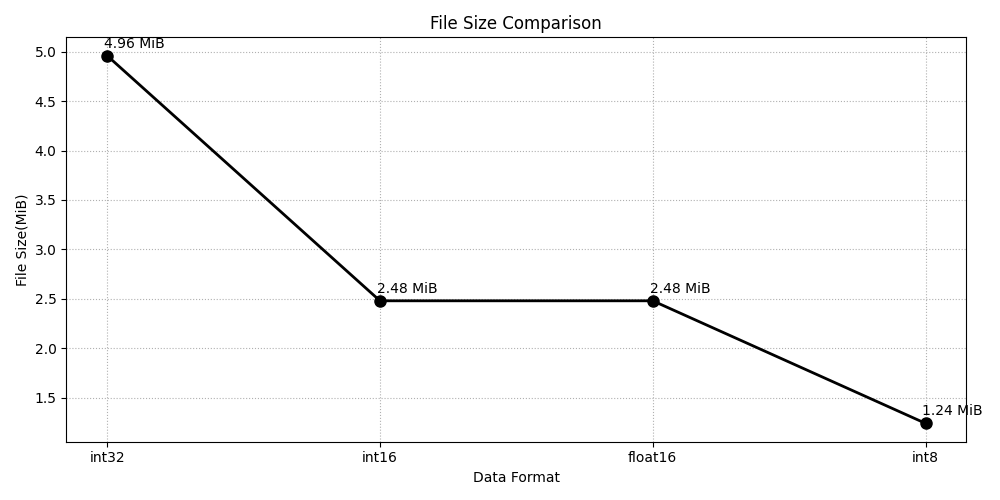
\includegraphics[height=0.4\textwidth]{assets/quantization/size_plot.png}
        \caption{File Size Comparision between Quantized Models}
        \label{fig:file-size-comparision}
    \end{figure}

    \begin{figure}[H]
        \centering
        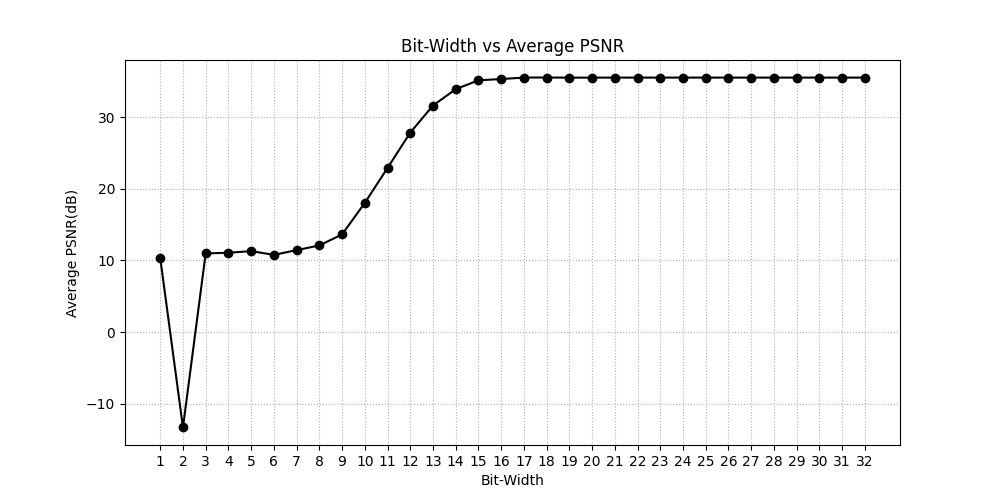
\includegraphics[height=0.4\textwidth]{assets/quantization/psnr.png}
        \caption{Average PSNR for Quantized Models}
        \label{fig:psnr-plot}
    \end{figure}

    \begin{figure}[H]
        \centering
        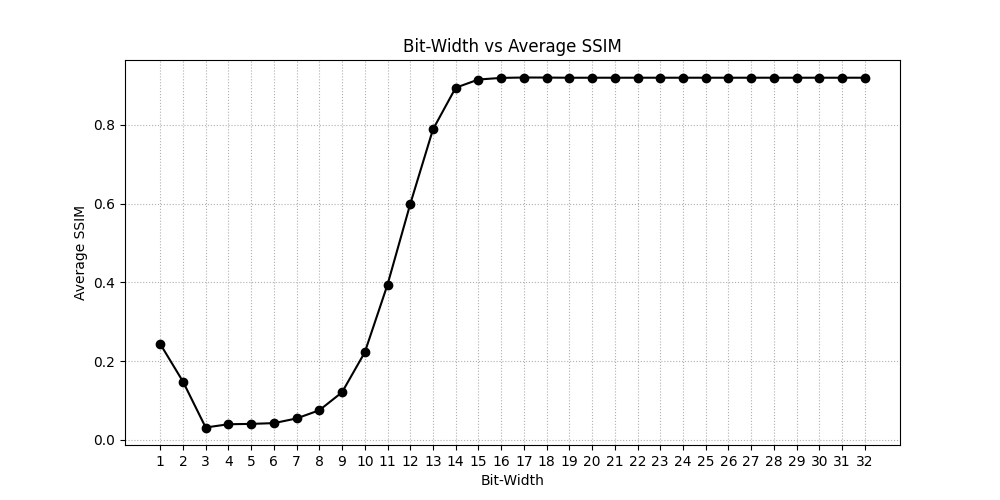
\includegraphics[height=0.4\textwidth]{assets/quantization/ssim.png}
        \caption{Average SSIM for Quantized Models}
        \label{fig:ssim-plot}
    \end{figure}

    \begin{figure}[H]
        \centering
        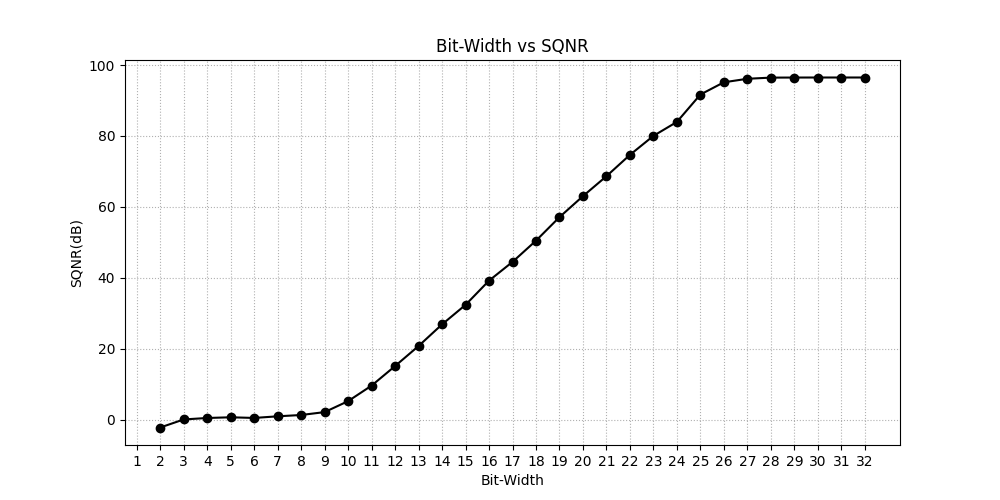
\includegraphics[height=0.4\textwidth]{assets/quantization/sqnr.png}
        \caption{SQNR for Quantized Models}
        \label{fig:sqnr-plot}
    \end{figure}

    The results, as observed from the graphs, show that quantizing the model to 16-bit integer results in reduction in file size. Moreover, both the \gls{ssim} and \gls{psnr} graphs indicate that reducing the bit-width initially affects these metrics, but from 16-bit onwards, the values stabilize, and further increase in bit-width has minimal impact on the model's accuracy. The \gls{sqnr} value for 16-bit quantization is also satisfactory. Given this balance between efficiency and performance, we chose to proceed with the 16-bit integer model for further experimentation and analysis. The results presented from this point onward are based on the 16-bit integer quantized model.

    \subsubsection{Visualization of Frames of Quantized Models}
    Here are the 10th frames of the videos generated by the student models for Video 1 after quantization to various bit-widths: 1, 4, 7, 10, 14, 16, 18, and 32.

    % \begin{figure}[H]
    %     \centering
    %     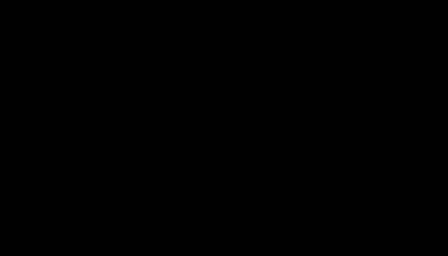
\includegraphics[height=0.4\textwidth]{assets/quantization/frames/rickq1.png}
    %     \caption{Frame 10 predicted by 1-bit Quantized Model}
    %     \label{fig:rickq1}
    % \end{figure}

    % \begin{figure}[H]
    %     \centering
    %     
\includegraphics[height=0.4\textwidth]{assets/quantization/frames/rickq4.png}
    %     \caption{Frame 10 predicted by 4-bit Quantized Model}
    %     \label{fig:rickq4}
    % \end{figure}

    % \begin{figure}[H]
    %     \centering
    %     
\includegraphics[height=0.4\textwidth]{assets/quantization/frames/rickq7.png}
    %     \caption{Frame 10 predicted by 7-bit Quantized Model}
    %     \label{fig:rickq7}
    % \end{figure}

    % \begin{figure}[H]
    %     \centering
    %     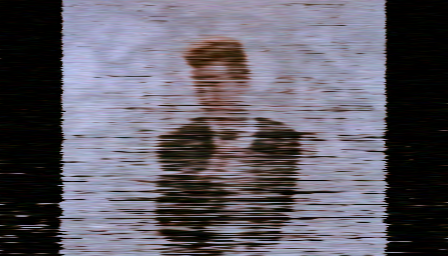
\includegraphics[height=0.4\textwidth]{assets/quantization/frames/rickq10.png}
    %     \caption{Frame 10 predicted by 10-bit Quantized Model}
    %     \label{fig:rickq10}
    % \end{figure}

    % \begin{figure}[H]
    %     \centering
    %     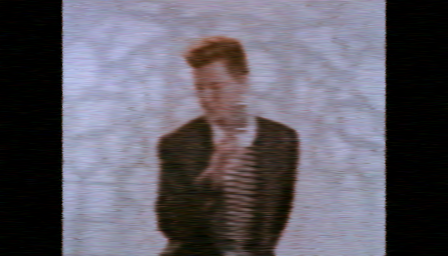
\includegraphics[height=0.4\textwidth]{assets/quantization/frames/rickq14.png}
    %     \caption{Frame 10 predicted by 14-bit Quantized Model}
    %     \label{fig:rickq14}
    % \end{figure}

    % \begin{figure}[H]
    %     \centering
    %     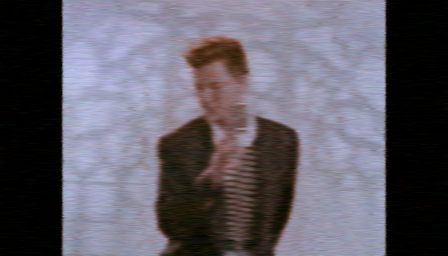
\includegraphics[height=0.4\textwidth]{assets/quantization/frames/rickq16.png}
    %     \caption{Frame 10 predicted by 16-bit Quantized Model}
    %     \label{fig:rickq16}
    % \end{figure}

    % \begin{figure}[H]
    %     \centering
    %     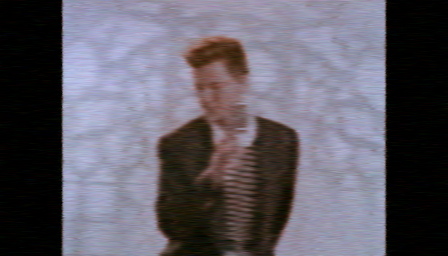
\includegraphics[height=0.4\textwidth]{assets/quantization/frames/rickq18.png}
    %     \caption{Frame 10 predicted by 18-bit Quantized Model}
    %     \label{fig:rickq18}
    % \end{figure}

    % \begin{figure}[H]
    %     \centering
    %     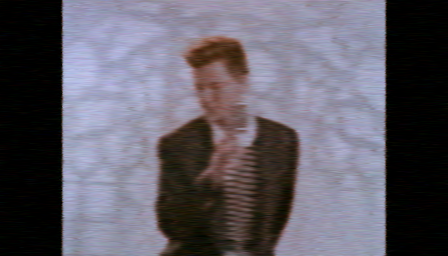
\includegraphics[height=0.4\textwidth]{assets/quantization/frames/rickq32.png}
    %     \caption{Frame 10 predicted by 32-bit Quantized Model}
    %     \label{fig:rickq32}
    % \end{figure}

    \begin{figure}[H]
        \centering
        \begin{subfigure}[b]{0.4\textwidth}
            \centering
            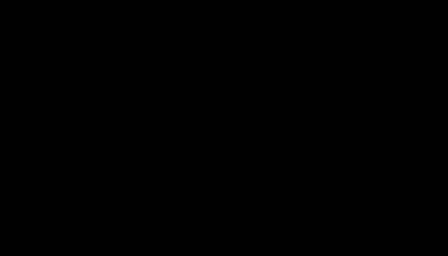
\includegraphics[width=\textwidth]{assets/quantization/frames/rickq1.png}
            \caption{1-bit Quantized Model}
            \label{fig:rickq1}
        \end{subfigure}
        \begin{subfigure}[b]{0.4\textwidth}
            \centering
            
\includegraphics[width=\textwidth]{assets/quantization/frames/rickq4.png}
            \caption{4-bit Quantized Model}
            \label{fig:rickq4}
        \end{subfigure}
    
        \begin{subfigure}[b]{0.4\textwidth}
            \centering
            
\includegraphics[width=\textwidth]{assets/quantization/frames/rickq7.png}
            \caption{7-bit Quantized Model}
            \label{fig:rickq7}
        \end{subfigure}
        \begin{subfigure}[b]{0.4\textwidth}
            \centering
            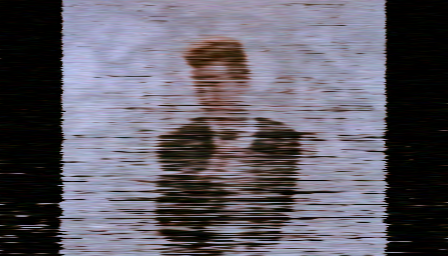
\includegraphics[width=\textwidth]{assets/quantization/frames/rickq10.png}
            \caption{10-bit Quantized Model}
            \label{fig:rickq10}
        \end{subfigure}
    
        \begin{subfigure}[b]{0.4\textwidth}
            \centering
            \includegraphics[width=\textwidth]{assets/quantization/frames/rickq14.png}
            \caption{14-bit Quantized Model}
            \label{fig:rickq14}
        \end{subfigure}
        \begin{subfigure}[b]{0.4\textwidth}
            \centering
            \includegraphics[width=\textwidth]{assets/quantization/frames/rickq16.png}
            \caption{16-bit Quantized Model}
            \label{fig:rickq16}
        \end{subfigure}
    
        \begin{subfigure}[b]{0.4\textwidth}
            \centering
            \includegraphics[width=\textwidth]{assets/quantization/frames/rickq18.png}
            \caption{18-bit Quantized Model}
            \label{fig:rickq18}
        \end{subfigure}
        \begin{subfigure}[b]{0.4\textwidth}
            \centering
            \includegraphics[width=\textwidth]{assets/quantization/frames/rickq32.png}
            \caption{32-bit Quantized Model}
            \label{fig:rickq32}
        \end{subfigure}
    
        \caption{Frame 10 predictions at different quantization levels}
        \label{fig:quantization_results}
    \end{figure}

    To provide a clear understanding of the impact of quantization on model output, we present visualizations of frames produced by the model after quantization to various bit-widths: 1, 4, 7, 10, 14, 16, 18, and 32. These frames illustrate how the quality of the output improves as the bit-width increases.

    By observing these visualizations, we can clearly see the trade-offs involved in reducing precision. Lower bit-widths (e.g., 1 and 4) result in significant degradation of image quality, making the output highly distorted or unrecognizable. As the bit-width increases to 7, 10, and 14, the images become progressively clearer. Notably, at 16-bit quantization, the output reaches a level where details are sufficiently preserved, offering a balance between efficiency and visual fidelity.

    Beyond 16-bit, further increases in bit-width (18 and 32) do not introduce drastic improvements that are perceivable to the naked eye. This observation justifies the choice of 16-bit quantization as an optimal trade-off between model efficiency and output quality.

    \subsubsection{Visualization of Weight Quantization}
    The weight quantization process is depicted in \autoref{fig:quantization-sample-weights}, which consists of 3x3 grid of some sample weights. An example calculation is shown for the first weight in \autoref{app:quantization-manual-conversion}.
    \begin{enumerate}[label=\textbf{\roman*.}]
        \item \textbf{Original Weights:} The weights before quantization.
        \item \textbf{Quantized Weights:} The weights after quantization into 8-bit integers.
        \item \textbf{Integer Representation:} The representation of quantized weights in int8 format.
    \end{enumerate}

    \begin{figure}[H]
        \centering
        \includegraphics[width=0.8\linewidth]{assets/quantization/quantization_sample_weights.png}
        \caption{Quantization Sample Weights}
        \label{fig:quantization-sample-weights}
    \end{figure}

    \pagebreak

    \subsubsection{Histogram of Student Models}
    \autoref{fig:hist-student-vid1} and \autoref{fig:hist-student-vid3} show the histogram of weights and biases of the Student Model of Video 1 and Video 3.

    \begin{figure}[H]
        \centering
        \includegraphics[width=\linewidth]{assets/quantization/histogram/histogram_vvsa_student.png}
        \caption{Histogram of Student Model:Video 1}
        \label{fig:hist-student-vid1}
    \end{figure}

    \begin{figure}[H]
        \centering
        \includegraphics[width=\linewidth]{assets/quantization/histogram/histogram_rick_student.png}
        \caption{Histogram of Student Model:Video 3}
        \label{fig:hist-student-vid3}
    \end{figure}

    These histograms visualize the distributions of weights and biases for two student models across different layers and components, such as audio and video branches, shared layers, and initial layers. The distributions are diverse, with weights generally exhibiting Gaussian-like shapes centered around zero. Meanwhile, biases show more uniformly or slightlys skewed distribution.
    \pagebreak


\section{\MakeUppercase{Remaining Tasks}}
The remaining tasks for the project involve applying knowledge distillation to the models of the three remaining videos and implementing quantization on the corresponding student models. Knowledge distillation will focus on transferring knowledge from the teacher models to the student models for these specific videos. The other three videos could not be trained earlier due to their larger size, which caused the student models to struggle in properly representing the videos.
Additionally, quantization will be applied to the student models corresponding to these three videos. Knowledge Distallation and Quantization for the first two videos has already been completed, and now the focus is on applying it to the remaining models. By addressing the challenges in knowledge distillation and completing the quantization process for these three videos, the project will meet its objectives of creating models for all videos in the dataset.
\pagebreak

% Appendix Section
\AppendixStyle{5.5em}
\section{\MakeUppercase{Appendices}}
    \setcounter{subsection}{0}
    \subsection{Project Schedule}
    \appendixnumbering{\Alph{subsection}}
    \label{app:project-schedule}

    \begin{figure}[H]
        \centering
        \includegraphics[angle=90, origin=c, height=0.5\textheight]{assets/Gantt-A.png}
        \caption{Gantt Chart for Major Project Part A}
        \label{fig:gantt-a}
    \end{figure}

    \begin{figure}[H]
        \centering
        \includegraphics[angle=90, origin=c, width=\linewidth]{assets/Gantt-B.png}
        \caption{Gantt Chart for Major Project Part B}
        \label{fig:gantt-b}
    \end{figure}
    
\pagebreak


\setcounter{subsection}{1}
\subsection{Forward and Backward Propagation}
\appendixnumbering{\Alph{subsection}}
\label{app:forward-backward-eqn}

\begin{figure}[H]
    \centering
    \includegraphics[width=\linewidth]{assets/32_32_neural.png}
    \caption{Neural Network Architecture for 32 by 32 image}
    \label{fig:32-32-neural}
\end{figure}

The below derivations have been done using \autoref{fig:32-32-neural} as reference.
\subsubsection{Forward Propagation}
\textbf{Step 1: Input Layer}
\begin{itemize}
  \item Input Vector $\mathbf{x}$: Dimension $2 \times 1$
  \item Weight Matrix $\mathbf{W}^{(in)}$: Dimension $2 \times 2$
  \item Bias Vector $\mathbf{b}^{(in)}$: Dimension $2 \times 1$
  \item Calculation:
  \begin{equation}
  \mathbf{z}^{(in)} = \mathbf{W}^{(in)} \mathbf{x} + \mathbf{b}^{(in)}
  \end{equation}
  \begin{equation}
  \mathbf{a}^{(in)} = \mathbf{z}^{(in)}
  \end{equation}
  Where $\mathbf{z}^{(in)}$ and $\mathbf{a}^{(in)}$ both have dimensions $2 \times 1$.
\end{itemize}


\textbf{Step 2: Hidden Layer 1}
\begin{itemize}
  \item Input Vector $\mathbf{x}$: Dimension $2 \times 1$
  \item Weight Matrix $\mathbf{W}^{(1)}$: Dimension $25 \times 2$
  \item Bias Vector $\mathbf{b}^{(1)}$: Dimension $25 \times 1$
  \item Calculation:
  \begin{equation}
  \mathbf{z}^{(1)} = \mathbf{W}^{(1)} \mathbf{x} + \mathbf{b}^{(1)}
  \end{equation}
  \begin{equation}
  \mathbf{a}^{(1)} = \sin(\mathbf{z}^{(1)})
  \end{equation}
  Where $\mathbf{z}^{(1)}$ and $\mathbf{a}^{(1)}$ both have dimensions $25 \times 1$.
\end{itemize}

\textbf{Step 3: Hidden Layer 2}
\begin{itemize}
  \item Weight Matrix $\mathbf{W}^{(2)}$: Dimension $25 \times 25$
  \item Bias Vector $\mathbf{b}^{(2)}$: Dimension $25 \times 1$
  \item Calculation:
  \begin{equation}
  \mathbf{z}^{(2)} = \mathbf{W}^{(2)} \mathbf{a}^{(1)} + \mathbf{b}^{(2)}
  \end{equation}
  \begin{equation}
  \mathbf{a}^{(2)} = \sin(\mathbf{z}^{(2)})
  \end{equation}
  Both $\mathbf{z}^{(2)}$ and $\mathbf{a}^{(2)}$ are $25 \times 1$.
\end{itemize}

\textbf{Step 4: Output Layer}
\begin{itemize}
  \item Weight Matrix $\mathbf{W}^{(3)}$: Dimension $3 \times 25$
  \item Bias Vector $\mathbf{b}^{(3)}$: Dimension $3 \times 1$
  \item Calculation:
  \begin{equation}
  \mathbf{z}^{(3)} = \mathbf{W}^{(3)} \mathbf{a}^{(2)} + \mathbf{b}^{(3)}
  \end{equation}
  \begin{equation}
  \mathbf{a}^{(3)} = \sin(\mathbf{z}^{(3)})
  \end{equation}
  Where $\mathbf{z}^{(3)}$ and $\mathbf{a}^{(3)}$ both have dimensions $3 \times 1$.
\end{itemize}


\subsubsection{Backpropagation}

\textbf{Step 1: Output Layer}
\begin{enumerate}[label=\textbf{\roman*.}]
  \item \textbf{Gradient of Loss with respect to output activations} $(\mathbf{a}^{(3)})$:
  
  Given the Mean Squared Error (MSE) loss function:
  \begin{equation}
  \text{Loss} = \frac{1}{2} \sum_{i=1}^{3} (y_i - a^{(3)}_i)^2
  \end{equation}
  Differentiate Loss w.r.t. $\mathbf{a}^{(3)}$:
  \begin{equation}
  \frac{\partial \text{Loss}}{\partial a^{(3)}_i} = a^{(3)}_i - y_i
  \end{equation}
  This will result in a vector $\mathbf{a}^{(3)} - \mathbf{y}$.

  \item \textbf{Gradient with respect to} $\mathbf{z}^{(3)}$ (using chain rule and recognizing $\mathbf{a}^{(3)} = \sin(\mathbf{z}^{(3)})$):
  \[
  \frac{\partial \text{Loss}}{\partial \mathbf{z}^{(3)}} = \frac{\partial \text{Loss}}{\partial \mathbf{a}^{(3)}} \cdot \frac{\partial \mathbf{a}^{(3)}}{\partial \mathbf{z}^{(3)}}
  \]
  Since $\frac{\partial a^{(3)}_i}{\partial z^{(3)}_i} = \cos(z^{(3)}_i)$, the gradient becomes:
  \begin{equation}
  \frac{\partial \text{Loss}}{\partial \mathbf{z}^{(3)}} = (\mathbf{a}^{(3)} - \mathbf{y}) \cdot \cos(\mathbf{z}^{(3)})
  \end{equation}

  \item \textbf{Gradient with respect to weights} $\mathbf{W}^{(3)}$ \textbf{and biases} $\mathbf{b}^{(3)}$:
  
  \[
  \frac{\partial \text{Loss}}{\partial \mathbf{W}^{(3)}} = \frac{\partial \text{Loss}}{\partial \mathbf{z}^{(3)}} \cdot \frac{\partial \mathbf{z}^{(3)}}{\partial \mathbf{W}^{(3)}}
  \]
  
  \[
  \frac{\partial \text{Loss}}{\partial \mathbf{W}^{(3)}} = \frac{\partial \text{Loss}}{\partial \mathbf{z}^{(3)}} \mathbf{a}^{(2)T}
  \]
  
  \begin{equation}
  \frac{\partial \text{Loss}}{\partial \mathbf{W}^{(3)}} = \left((\mathbf{a}^{(3)} - \mathbf{y}) \cdot \cos(\mathbf{z}^{(3)})\right) \mathbf{a}^{(2)T}
  \end{equation}


  \[
  \frac{\partial \text{Loss}}{\partial \mathbf{b}^{(3)}} = \frac{\partial \text{Loss}}{\partial \mathbf{z}^{(3)}} \cdot \frac{\partial \mathbf{z}^{(3)}}{\partial \mathbf{b}^{(3)}}
  \]

  \[
  \frac{\partial \text{Loss}}{\partial \mathbf{b}^{(3)}} = \frac{\partial \text{Loss}}{\partial \mathbf{z}^{(3)}}
  \]

  \begin{equation}
  \frac{\partial \text{Loss}}{\partial \mathbf{b}^{(3)}} = (\mathbf{a}^{(3)} - \mathbf{y}) \cdot \cos(\mathbf{z}^{(3)})
  \end{equation}
  
\end{enumerate}

\textbf{Step 2: Hidden Layer 2}
\begin{enumerate}[label=\textbf{\roman*.}]
  \item \textbf{Gradient with respect to activations} $\mathbf{a}^{(2)}$:
    \[
  \frac{\partial \text{Loss}}{\partial \mathbf{a}^{(2)}} = \frac{\partial \text{Loss}}{\partial \mathbf{z}^{(3)}} \cdot \frac{\partial \mathbf{z}^{(3)}}{\partial \mathbf{a}^{(2)}}
  \]
  \[
  \frac{\partial \text{Loss}}{\partial \mathbf{a}^{(2)}} = \mathbf{W}^{(3)T} \frac{\partial \text{Loss}}{\partial \mathbf{z}^{(3)}}
  \]
  \begin{equation}
  \frac{\partial \text{Loss}}{\partial \mathbf{a}^{(2)}} = \mathbf{W}^{(3)T} \left((\mathbf{a}^{(3)} - \mathbf{y}) \cdot \cos(\mathbf{z}^{(3)})\right)
  \end{equation}
  \item \textbf{Gradient with respect to} $\mathbf{z}^{(2)}$:
    \[
  \frac{\partial \text{Loss}}{\partial \mathbf{z}^{(2)}} = \frac{\partial \text{Loss}}{\partial \mathbf{a}^{(2)}} \cdot \frac{\partial \mathbf{a}^{(2)}}{\partial \mathbf{z}^{(2)}}
  \]
  \[
  \frac{\partial \text{Loss}}{\partial \mathbf{z}^{(2)}} = \frac{\partial \text{Loss}}{\partial \mathbf{a}^{(2)}} \cdot \cos(\mathbf{z}^{(2)})
  \]
  \begin{equation}
  \frac{\partial \text{Loss}}{\partial \mathbf{z}^{(2)}} = \left(\mathbf{W}^{(3)T} \left((\mathbf{a}^{(3)} - \mathbf{y}) \cdot \cos(\mathbf{z}^{(3)})\right)\right) \cdot \cos(\mathbf{z}^{(2)})
  \end{equation}

  \item \textbf{Gradient with respect to weights} $\mathbf{W}^{(2)}$ \textbf{and biases} $\mathbf{b}^{(2)}$:
  \[
  \frac{\partial \text{Loss}}{\partial \mathbf{W}^{(2)}} = \frac{\partial \text{Loss}}{\partial \mathbf{z}^{(2)}} \cdot \frac{\partial \mathbf{z}^{(2)}}{\partial \mathbf{W}^{(2)}}
  \]
  \[
  \frac{\partial \text{Loss}}{\partial \mathbf{W}^{(2)}} = \frac{\partial \text{Loss}}{\partial \mathbf{z}^{(2)}} \mathbf{a}^{(1)T}
  \]

  \begin{equation}
  \frac{\partial \text{Loss}}{\partial \mathbf{W}^{(2)}} = \left(\left(\mathbf{W}^{(3)T} \left((\mathbf{a}^{(3)} - \mathbf{y}) \cdot \cos(\mathbf{z}^{(3)})\right)\right) \cdot \cos(\mathbf{z}^{(2)})\right) \mathbf{a}^{(1)T}
  \end{equation}
 

   \[
  \frac{\partial \text{Loss}}{\partial \mathbf{b}^{(2)}} = \frac{\partial \text{Loss}}{\partial \mathbf{z}^{(2)}} \cdot \frac{\partial \mathbf{z}^{(2)}}{\partial \mathbf{b}^{(2)}}
  \]
  \[
  \frac{\partial \text{Loss}}{\partial \mathbf{b}^{(2)}} = \frac{\partial \text{Loss}}{\partial \mathbf{z}^{(2)}}
  \]

  \begin{equation}
  \frac{\partial \text{Loss}}{\partial \mathbf{b}^{(2)}} = \left(\mathbf{W}^{(3)T} \left((\mathbf{a}^{(3)} - \mathbf{y}) \cdot \cos(\mathbf{z}^{(3)})\right)\right) \cdot \cos(\mathbf{z}^{(2)})
  \end{equation}
\end{enumerate}

\textbf{Step 3: Hidden Layer 1}
\begin{enumerate}[label=\textbf{\roman*.}]
  \item \textbf{Gradient with respect to activations} $\mathbf{a}^{(1)}$:
      \[
  \frac{\partial \text{Loss}}{\partial \mathbf{a}^{(1)}} = \frac{\partial \text{Loss}}{\partial \mathbf{z}^{(2)}} \cdot \frac{\partial \mathbf{z}^{(2)}}{\partial \mathbf{a}^{(1)}}
  \]
  
  \[
  \frac{\partial \text{Loss}}{\partial \mathbf{a}^{(1)}} = \mathbf{W}^{(2)T} \frac{\partial \text{Loss}}{\partial \mathbf{z}^{(2)}}
  \]
  \begin{equation}
  \frac{\partial \text{Loss}}{\partial \mathbf{a}^{(1)}} = \mathbf{W}^{(2)T} \left(\left(\mathbf{W}^{(3)T} \left((\mathbf{a}^{(3)} - \mathbf{y}) \cdot \cos(\mathbf{z}^{(3)})\right)\right) \cdot \cos(\mathbf{z}^{(2)})\right)
  \end{equation}

  \item \textbf{Gradient with respect to} $\mathbf{z}^{(1)}$:
    \[
  \frac{\partial \text{Loss}}{\partial \mathbf{z}^{(1)}} = \frac{\partial \text{Loss}}{\partial \mathbf{a}^{(1)}} \cdot \frac{\partial \mathbf{a}^{(1)}}{\partial \mathbf{z}^{(1)}}
  \]

  \[
  \frac{\partial \text{Loss}}{\partial \mathbf{z}^{(1)}} = \frac{\partial \text{Loss}}{\partial \mathbf{a}^{(1)}} \cdot \cos(\mathbf{z}^{(1)})
  \]
  \begin{equation}
  \frac{\partial \text{Loss}}{\partial \mathbf{z}^{(1)}} = \left(\mathbf{W}^{(2)T} \left(\left(\mathbf{W}^{(3)T} \left((\mathbf{a}^{(3)} - \mathbf{y}) \cdot \cos(\mathbf{z}^{(3)})\right)\right) \cdot \cos(\mathbf{z}^{(2)})\right)\right) \cdot \cos(\mathbf{z}^{(1)})
  \end{equation}

  \item \textbf{Gradient with respect to weights} $\mathbf{W}^{(1)}$ \textbf{and biases} $\mathbf{b}^{(1)}$:
       \[
  \frac{\partial \text{Loss}}{\partial \mathbf{W}^{(1)}} = \frac{\partial \text{Loss}}{\partial \mathbf{z}^{(1)}} \cdot \frac{\partial \mathbf{z}^{(1)}}{\partial \mathbf{W}^{(1)}}
  \]
  \[
  \frac{\partial \text{Loss}}{\partial \mathbf{W}^{(1)}} = \frac{\partial \text{Loss}}{\partial \mathbf{z}^{(1)}} \mathbf{x}^T
  \]
  \begin{equation}
  \frac{\partial \text{Loss}}{\partial \mathbf{W}^{(1)}} = \left(\left(\mathbf{W}^{(2)T} \left(\left(\mathbf{W}^{(3)T} \left((\mathbf{a}^{(3)} - \mathbf{y}) \cdot \cos(\mathbf{z}^{(3)})\right)\right) \cdot \cos(\mathbf{z}^{(2)})\right)\right) \cdot \cos(\mathbf{z}^{(1)})\right) \mathbf{x}^T
  \end{equation}

  
         \[
  \frac{\partial \text{Loss}}{\partial \mathbf{b}^{(1)}} = \frac{\partial \text{Loss}}{\partial \mathbf{z}^{(1)}} \cdot \frac{\partial \mathbf{z}^{(1)}}{\partial \mathbf{b}^{(1)}}
  \]
  \[
  \frac{\partial \text{Loss}}{\partial \mathbf{b}^{(1)}} = \frac{\partial \text{Loss}}{\partial \mathbf{z}^{(1)}}
  \]
  \begin{equation}
  \frac{\partial \text{Loss}}{\partial \mathbf{b}^{(1)}} = \left(\mathbf{W}^{(2)T} \left(\left(\mathbf{W}^{(3)T} \left((\mathbf{a}^{(3)} - \mathbf{y}) \cdot \cos(\mathbf{z}^{(3)})\right)\right) \cdot \cos(\mathbf{z}^{(2)})\right)\right) \cdot \cos(\mathbf{z}^{(1)})
  \end{equation}
\end{enumerate}

\textbf{Step 4: Input Layer}
\begin{enumerate}[label=\textbf{\roman*.}]
  \item \textbf{Gradient with respect to activations} $\mathbf{a}^{(in)}$:
      \[
  \frac{\partial \text{Loss}}{\partial \mathbf{a}^{(in)}} = \frac{\partial \text{Loss}}{\partial \mathbf{z}^{(1)}} \cdot \frac{\partial \mathbf{z}^{(1)}}{\partial \mathbf{a}^{(in)}}
  \]
  
  \[
  \frac{\partial \text{Loss}}{\partial \mathbf{a}^{(in)}} = \mathbf{W}^{(1)T} \frac{\partial \text{Loss}}{\partial \mathbf{z}^{(1)}}
  \]
  \begin{equation}
  \frac{\partial \text{Loss}}{\partial \mathbf{a}^{(in)}} =\mathbf{W}^{(1)T}\left(\left(\mathbf{W}^{(2)T} \left(\left(\mathbf{W}^{(3)T} \left((\mathbf{a}^{(3)} - \mathbf{y}) \cdot \cos(\mathbf{z}^{(3)})\right)\right) \cdot \cos(\mathbf{z}^{(2)})\right)\right) \cdot \cos(\mathbf{z}^{(1)})\right) 
  \end{equation}

  \item \textbf{Gradient with respect to} $\mathbf{z}^{(in)}$:
    \[
  \frac{\partial \text{Loss}}{\partial \mathbf{z}^{(in)}} = \frac{\partial \text{Loss}}{\partial \mathbf{a}^{(in)}} \cdot \frac{\partial \mathbf{a}^{(in)}}{\partial \mathbf{z}^{(in)}}
  \]

  \[
  \frac{\partial \text{Loss}}{\partial \mathbf{z}^{(in)}} = \frac{\partial \text{Loss}}{\partial \mathbf{a}^{(in)}} \cdot \cos(\mathbf{z}^{(in)})
  \]
  \begin{equation}
  \frac{\partial \text{Loss}}{\partial \mathbf{z}^{(in)}} = \mathbf{W}^{(1)T}\left(\left(\mathbf{W}^{(2)T} \left(\left(\mathbf{W}^{(3)T} \left((\mathbf{a}^{(3)} - \mathbf{y}) \cdot \cos(\mathbf{z}^{(3)})\right)\right) \cdot \cos(\mathbf{z}^{(2)})\right)\right) \cdot \cos(\mathbf{z}^{(1)})\right)  \cdot \cos(\mathbf{z}^{(in)})
  \end{equation}

  \item \textbf{Gradient with respect to weights} $\mathbf{W}^{(in)}$ \textbf{and biases} $\mathbf{b}^{(in)}$:
       \[
  \frac{\partial \text{Loss}}{\partial \mathbf{W}^{(in)}} = \frac{\partial \text{Loss}}{\partial \mathbf{z}^{(in)}} \cdot \frac{\partial \mathbf{z}^{(in)}}{\partial \mathbf{W}^{(in)}}
  \]
  \begin{equation}
  \frac{\partial \text{Loss}}{\partial \mathbf{W}^{(in)}} = \frac{\partial \text{Loss}}{\partial \mathbf{z}^{(in)}} \mathbf{x}^T
  \end{equation}
  %   \[
  % \frac{\partial \text{Loss}}{\partial \mathbf{W}^{(in)}} = \mathbf{W}^{(1)T}\left(\left(\mathbf{W}^{(2)T} \left(\left(\mathbf{W}^{(3)T} \left((\mathbf{a}^{(3)} - \mathbf{y}) \cdot \cos(\mathbf{z}^{(3)})\right)\right) \cdot \cos(\mathbf{z}^{(2)})\right)\right) \cdot \cos(\mathbf{z}^{(1)})\right)  \cdot \cos(\mathbf{z}^{(in)}) \mathbf{x}^T
  % \]

         \[
  \frac{\partial \text{Loss}}{\partial \mathbf{b}^{(in)}} = \frac{\partial \text{Loss}}{\partial \mathbf{z}^{(in)}} \cdot \frac{\partial \mathbf{z}^{(in)}}{\partial \mathbf{b}^{(in)}}
  \]
  \begin{equation}
  \frac{\partial \text{Loss}}{\partial \mathbf{b}^{(in)}} = \frac{\partial \text{Loss}}{\partial \mathbf{z}^{(in)}}
  \end{equation}
% \[
%   \frac{\partial \text{Loss}}{\partial \mathbf{b}^{(in)}} = \mathbf{W}^{(1)T}\left(\left(\mathbf{W}^{(2)T} \left(\left(\mathbf{W}^{(3)T} \left((\mathbf{a}^{(3)} - \mathbf{y}) \cdot \cos(\mathbf{z}^{(3)})\right)\right) \cdot \cos(\mathbf{z}^{(2)})\right)\right) \cdot \cos(\mathbf{z}^{(1)})\right)  \cdot \cos(\mathbf{z}^{(in)})
%   \]
\end{enumerate}

\pagebreak


\setcounter{subsection}{2}
\subsection{Arcsine Distribution on [-1, 1]}
\label{app:arcsine-distribution}
\appendixnumbering{\Alph{subsection}}

\textbf{Probability Density Function (PDF)}\\
The PDF of the arcsine distribution on the interval \((-1, 1)\) is given by:
\begin{equation}
    f(x) = \frac{1}{\pi \sqrt{1-x^2}}
\end{equation}

\textbf{Cumulative Distribution Function (CDF)}\\
The cumulative distribution function (CDF), \( F(x) \), is defined as the integral of the probability density function (PDF) from the lower bound of the interval to \( x \):
\begin{equation}
    F(x) = \int_{-1}^{x} f(t) \, dt
\end{equation}

Given the PDF for the arcsine distribution:
\[
f(x) = \frac{1}{\pi \sqrt{1-x^2}}
\]

we need to integrate this PDF from -1 to \( x \):
\[
F(x) = \int_{-1}^{x} \frac{1}{\pi \sqrt{1-t^2}} \, dt
\]

To solve this integral, we use the substitution \( t = \sin \theta \).\\
Thus, \( dt = \cos \theta \, d\theta \) and \( \sqrt{1-t^2} = \sqrt{1-\sin^2 \theta} = \cos \theta \).\\
When \( t = -1 \), \( \theta = -\frac{\pi}{2} \).\\
When \( t = x \), \( \theta = \arcsin x \).\\
Therefore, the integral becomes:
\[
F(x) = \int_{-\frac{\pi}{2}}^{\arcsin x} \frac{1}{\pi \cos \theta} \cos \theta \, d\theta = \int_{-\frac{\pi}{2}}^{\arcsin x} \frac{1}{\pi} \, d\theta
\]

\[
F(x) = \frac{1}{\pi} \int_{-\frac{\pi}{2}}^{\arcsin x} d\theta = \frac{1}{\pi} \left[ \theta \right]_{-\frac{\pi}{2}}^{\arcsin x}
\]

\[
F(x) = \frac{1}{\pi} \left( \arcsin x - \left( -\frac{\pi}{2} \right) \right)
\]

\[
F(x) = \frac{1}{\pi} \arcsin x + \frac{1}{\pi} \cdot \frac{\pi}{2}
\]

\[
F(x) = \frac{1}{\pi} \arcsin x + \frac{1}{2}
\]

Thus, the CDF of the arcsine distribution on \([-1, 1]\) is:
\begin{equation}
    F(x) = \frac{1}{\pi} \arcsin(x) + \frac{1}{2}
\end{equation}

\textbf{Mean}\\
The mean \(\mu\) of the distribution is given by:
\begin{equation}
    \mu = \int_{-1}^{1} x f(x) \, dx = \int_{-1}^{1} x \cdot \frac{1}{\pi \sqrt{1-x^2}} \, dx
\end{equation}
This integral evaluates to zero because \( x \cdot f(x) \) is an odd function integrated over a symmetric interval around zero:
\begin{equation}
    \mu = 0
\end{equation}

\textbf{Variance}\\
The variance \(\sigma^2\) is calculated as:
\begin{equation}
    \sigma^2 = \mathbf{E}[X^2] - (\mathbf{E}[X])^2
\end{equation}
Since \(\mathbf{E}[X] = 0\), we have:
\[
\mathbf{E}[X^2] = \int_{-1}^{1} x^2 f(x) \, dx = \int_{-1}^{1} x^2 \cdot \frac{1}{\pi \sqrt{1-x^2}} \, dx
\]
By symmetry and properties of the arcsine distribution, this integral evaluates to:
\[
\mathbf{E}[X^2] = \frac{1}{2}
\]
Thus, the variance is:
\begin{equation}
    \sigma^2 = \frac{1}{2} - 0^2 = \frac{1}{2}
\end{equation}

\pagebreak

\setcounter{subsection}{3}
\subsection{IEEE 754 Floating Point Representation}
\label{app:ieee-754-fp32}
\appendixnumbering{\Alph{subsection}}

\begin{figure}[H]
    \centering
    \includegraphics[width=\linewidth]{assets/weightsviz.png}
    \caption{Final Weights for Audio 1}
    \label{fig:final-weights-a1}
\end{figure}
\begin{table}[H]
    \caption{Derivation and PyTorch Notation for Weights and Biases}
    \centering
    \resizebox{\textwidth}{!}{%
    \begin{tabular}{|l|l|c|c|c|c|}
    \hline
    \multicolumn{2}{|c|}{\textbf{Layer}} & \multicolumn{2}{|c|}{\textbf{Derivation Notation}} & \multicolumn{2}{|c|}{\textbf{PyTorch Notation}} \\ \hline
    \textbf{From} & \textbf{To} & \textbf{Weights} & \textbf{Biases} & \textbf{Weights} & \textbf{Biases} \\ \hline
    Input & Input Layer & $W_{in}$ & $b_{in}$ & \texttt{net.net.0.0.weight} & \texttt{net.net.0.0.bias} \\ \hline
    Input Layer & Hidden 1 & $W^{(1)}$ & $b^{(1)}$ & \texttt{net.net.1.0.weight} & \texttt{net.net.1.0.bias} \\ \hline
    Hidden 1 & Hidden 2 & $W^{(2)}$ & $b^{(2)}$ & \texttt{net.net.2.0.weight} & \texttt{net.net.2.0.bias} \\ \hline
    Hidden 2 & Hidden 3 & $W^{(3)}$ & $b^{(3)}$ & \texttt{net.net.3.0.weight} & \texttt{net.net.3.0.bias} \\ \hline
    Hidden 3 & Hidden 4 & $W^{(4)}$ & $b^{(4)}$ & \texttt{net.net.4.0.weight} & \texttt{net.net.4.0.bias} \\ \hline
    Hidden 4 & Output & $W_{out}$ & $b_{out}$ & \texttt{net.net.5.0.weight} & \texttt{net.net.5.0.bias} \\ \hline
    \end{tabular}%
    }
    \label{table:weights_biases}
    \end{table}
    
    
To represent the number \( 0.9146 \) in IEEE 754 single precision floating-point format:

1. \textbf{Convert to Binary:}
\[
0.9146_{10} \approx 0.111010100010001100111010_2
\]

2. \textbf{Normalize the Binary Number:}
\[
0.111010100010001100111010_2 = 1.11010100010001100111010 \times 2^{-1}
\]

3. \textbf{Bias the Exponent:}
\[
\text{Exponent} = -1 + 127 = 126
\]

In binary:
\[
126_{10} = 01111110_2
\]

4. \textbf{IEEE 754 Representation:}
\begin{equation}
    \begin{array}{|c|c|c|}
        \hline
        \text{Sign Bit} & \text{Exponent} & \text{Mantissa} \\
        \hline
        0 & 01111110 & 11010100010001100111010 \\
        \hline
    \end{array}
\end{equation}

5. \textbf{Convert IEEE 754 Representation to Decimal:}
\begin{itemize}
    \item \textbf{Sign Bit}: 0 (indicating a positive number)
    \item \textbf{Exponent}: \(01111110_2\) in binary, which is 126 in decimal.
    \item \textbf{Bias}: 127
    \item \textbf{Actual Exponent}: \(126 - 127 = -1\)
    \item \textbf{Mantissa}: \(1.11010100010001100111010_2\) (implicit leading 1 added)
\end{itemize}

\textbf{Calculate the Decimal Value:}
\[
\text{Value} = (-1)^{\text{sign}} \times 1.\text{Mantissa} \times 2^{\text{Actual Exponent}}
\]
\[
\text{Value} = (-1)^0 \times 1.11010100010001100111010_2 \times 2^{-1}
\]

Convert \(1.11010100010001100111010_2\) to decimal:
\begin{align*}
    1.11010100010001100111010_2 &= 1 + 0.5 + 0.25 + 0.0625 + 0.015625 + 9.765625 \times 10^{-4}\\
        &\begin{aligned}
        % &1 + 0.5 + 0.25 + 0.0625 + 0.015625 + 9.765625 \times 10^{-4}\\
        &+ 6.103515625 \times 10^{-5} + 3.051757813 \times 10^{-5} + \\
        & 3.814697266 \times 10^{-6} + 1.907348633 \times 10^{-6}\\
        &+ 9.536743164 \times 10^{-7} + 2.384185791 \times 10^{-7}\\
    \end{aligned}\\
        &= 1.829200029373168945312
\end{align*}
\begin{equation}
    \begin{aligned}
        \text{Value} &= 1.829200029373168945312 \times 2^{-1}\\
        &= 1.829200029373168945312 \times 0.5\\
        &= 0.914600014686584472656
    \end{aligned}
\end{equation}

The discrepancy arises because the true value of \(0.9146\) cannot be exactly represented in binary. The value stored in IEEE 754 format is \(0.914600014686584472656\), which is very close to the original value \(0.9146\), with the difference due to rounding in the conversion process.

\pagebreak


\setcounter{subsection}{4}
\subsection{Custom Floating-Point Format}
\label{app:custom-floating-point-formats}
\appendixnumbering{\Alph{subsection}}

\begin{enumerate}[label=\textbf{\roman*.}]
    \item \textbf{FP32:}
    FP32 (32-bit Floating Point) is the standard floating-point format widely used in many applications, offering a good balance of precision and dynamic range. It consists of 1 sign bit, 8 exponent bits, and 23 mantissa bits, offering a high degree of precision.
    \[
    \begin{array}{|c|c|c|}
        \hline
        \text{Sign Bit} & \text{Exponent} & \text{Mantissa} \\
        \hline
        1 \text{bit} & 8 \text{bits} & 23 \text{bits} \\
        \hline
    \end{array}
    \]
    FP32 is commonly used in applications where high precision is necessary, such as scientific computing, 3D graphics, and high-performance computing.

    \textbf{Calculation of Minimum and Maximum values:}
    \[
    \text{Value} = (-1)^{\text{sign}} \times 1.\text{Mantissa} \times 2^{\text{Exponent - 127}}
    \]

    For maximum value:\\
    Sign = 0 \\
    Exponent = 11111110 (All 1s is reserved for NaN values) \\
    Mantissa = 11111111111111111111111 
    \[
        \begin{aligned}
            \text{Maximum Value} &= (-1)^{0} \times 1.11111111111111111111111 \times 2^{11111110} \\
            & \approx (1) \times 1.999999880 \times 2^{254 - 127} \\
            & \approx 1.999999880 \times 2^{127} \\
            & \approx 3.4028235 \times 10^{38}
        \end{aligned}
    \]

    For minimum value:\\
    The minimum value that can be represented in FP32 is a subnormal number. To indicate a subnormal number, all 0s are stored in Exponent. \\
    Sign = 1 \\
    Exponent = 00000000 (Indicating a subnormal number)\\
    Mantissa = 00000000000000000000001
    \[
        \begin{aligned}
            \text{Minimum Value} &= (-1)^{1} \times 0.00000000000000000000001 \times 2^{-126} \\
            & = (-1) \times 2^{-23} \times 2^{-126} \\
            & =  2^{-149} \\
            & \approx -1.401298 \times 10^{-45}
        \end{aligned}
    \]
    The minimum normal value can also be calculated as : \\
    Sign = 1 \\
    Exponent = 00000001 (Smallest non-zero exponent for normalized numbers)\\
    Mantissa = 00000000000000000000000
    \[
        \begin{aligned}
            \text{Minimum Value} &= (-1)^{1} \times 1 \times 2^{-126} \\
            & = (-1) \times (1) \times 2^{-126} \\
            & =  -2^{-126} \\
            & \approx -1.1754944 \times 10^{-38}
        \end{aligned}
    \]

    \begin{table}[H]
        \centering
        \caption{Advantages and Disadvantages of FP32}
        \label{tab:fp32}
        \begin{tabular}{|p{6cm}|p{6cm}|}
        \hline
        \textbf{Advantages} & \textbf{Disadvantages} \\
        \hline
        High Precision: Suitable for applications requiring high numerical accuracy. & Computationally Expensive: Requires more memory and processing power. \\
        \hline
        Wide Dynamic Range: Supports a wide range of values. & Slower Operations: More resource-intensive than lower precision formats. \\
        \hline
        \end{tabular}
    \end{table}

\item \textbf{FP16:}
    FP16 (16-bit Floating Point) is a lower-precision floating-point format that sacrifices some precision in favor of reducing memory usage and improving computation speed. It uses 1 sign bit, 5 exponent bits, and 10 mantissa bits.
    \[
    \begin{array}{|c|c|c|}
        \hline
        \text{Sign Bit} & \text{Exponent} & \text{Mantissa} \\
        \hline
        1 \text{bit} & 5 \text{bits} & 10 \text{bits} \\
        \hline
    \end{array}
    \]
    
    FP16 is commonly used in machine learning tasks to speed up training while reducing memory consumption.

    \textbf{Calculation of Minimum and Maximum values:}
    \[
    \text{Value} = (-1)^{\text{sign}} \times 1.\text{Mantissa} \times 2^{\text{Exponent - 15}}
    \]

    For maximum value:\\
    Sign = 0 \\
    Exponent = 11110 (All 1s is reserved for NaN values) \\
    Mantissa = 1111111111 
    \[
        \begin{aligned}
            \text{Maximum Value} &= (-1)^{0} \times 1.1111111111 \times 2^{11110} \\
            & \approx (1) \times 1.999999880 \times 2^{30 - 15} \\
            & \approx 1.999999880 \times 2^{15} \\
            & \approx 65504
        \end{aligned}
    \]

    For minimum value:\\
    The minimum value that can be represented in FP16 is a subnormal number. To indicate a subnormal number, all 0s are stored in Exponent. \\
    Sign = 1 \\
    Exponent = 00000 (Indicating a subnormal number)\\
    Mantissa = 0000000001
    \[
        \begin{aligned}
            \text{Minimum Value} &= (-1)^{1} \times 0.0000000001 \times 2^{-14} \\
            & = (-1) \times 2^{-10} \times 2^{-14} \\
            & =  2^{-24} \\
            & \approx -5.960464477 \times 10^{-8}
        \end{aligned}
    \]
    The minimum normal value can also be calculated as : \\
    Sign = 1 \\
    Exponent = 00001 (Smallest non-zero exponent for normalized numbers)\\
    Mantissa = 0000000000
    \[
        \begin{aligned}
            \text{Minimum Value} &= (-1)^{1} \times 1 \times 2^{-14} \\
            & = (-1) \times (1) \times 2^{-15} \\
            & =  -2^{-15} \\
            & \approx -3.051757 \times 10^{-5}
        \end{aligned}
    \]

 
    \begin{table}[H]
        \centering
        \caption{Advantages and Disadvantages of FP16}
        \label{tab:fp16}
        \begin{tabular}{|p{6cm}|p{6cm}|}
        \hline
        \textbf{Advantages} & \textbf{Disadvantages} \\
        \hline
        Reduced Memory Usage: Saves memory space, especially for large models. & Lower Precision: Less accurate for some tasks requiring high precision. \\
        \hline
        Faster Computation: Reduces processing time in many tasks. & Limited Dynamic Range: Smaller exponent range than FP32. \\
        \hline
        \end{tabular}
    \end{table}

\item \textbf{FP8:}
    FP8 (8-bit Floating Point) is an extremely low-precision format that is mainly used in specialized applications where extreme memory efficiency is required. It uses 1 sign bit, 4 exponent bits, and 3 mantissa bits.
    \[
    \begin{array}{|c|c|c|}
        \hline
        \text{Sign Bit} & \text{Exponent} & \text{Mantissa} \\
        \hline
        1 \text{bit} & 4 \text{bits} & 3 \text{bits} \\
        \hline
    \end{array}
    \]
    The above example is of E4M3 variant. It also has another variant named E5M2 which has 1 sign bit, 5 exponent bits and only 2 mantissa bits.
    
    FP8 is used in contexts like model quantization or inference tasks, where the trade-off between precision and speed can be adjusted.

    \textbf{Calculation of Minimum and Maximum values(E4M3):}
    
    \[
    \text{Value} = (-1)^{\text{sign}} \times 1.\text{Mantissa} \times 2^{\text{Exponent - 7}}
    \]

    For maximum value:\\
    Sign = 0 \\
    Exponent = 1111 \\
    Mantissa = 110
    \[
    \begin{aligned}
        \text{Maximum Value} &= (-1)^{0} \times 1.110 \times 2^{1110} \\
        &= (1) \times 1.75 \times 2^{15 - 7} \\
        &= 1.75 \times 2^{8} \\
        &= 1.75 \times 128 \\
        &= 448
    \end{aligned}
    \]
    
    For minimum value:\\
    The minimum value that can be represented in FP8 is a subnormal number. To indicate a subnormal number, all 0s are stored in Exponent. \\
    Sign = 1 \\
    Exponent = 0000 (All 1s is reserved for NaN values) \\
    Mantissa = 111 
    \[
    \begin{aligned}
        \text{Minimum Value} &= (-1)^{1} \times 0.111 \times 2^{-6} \\
        &= (-1) \times 0.875 \times 2^{-6} \\
        &= -1.875 \times 2^{-6} \\
        &= -1.875 \times 128 \\
        & \approx -1.36 \times 10^{-2}
    \end{aligned}
    \]
    The minimum normal value can also be calculated as : \\
    Sign = 1 \\
    Exponent = 0001 (Smallest non-zero exponent for normalized numbers)\\
    Mantissa = 000
    \[
        \begin{aligned}
            \text{Minimum Value} &= (-1)^{1} \times 1 \times 2^{-6} \\
            & =  -2^{-6} \\
            & \approx -1.56 \times 10^{-2}
        \end{aligned}
    \]

 
    \begin{table}[H]
        \centering
        \caption{Advantages and Disadvantages of FP8}
        \label{tab:fp8}
        \begin{tabular}{|p{6cm}|p{6cm}|}
        \hline
        \textbf{Advantages} & \textbf{Disadvantages} \\
        \hline
        Extremely Low Memory Usage: Minimizes memory requirements. & Very Low Precision: Inadequate for tasks requiring high accuracy. \\
        \hline
        Faster Computation: Significantly increases speed in simple operations. & Small Dynamic Range: Can lead to overflows and underflows. \\
        \hline
        Reduced data movement and simpler arithmetic operations lead to lower power consumption. & Limited Support : FP8 is not yet supported by all hardware and software \\
        \hline
        \end{tabular}
    \end{table}

    \item \textbf{INT8:}
    INT8 (8-bit Integer) is a format that uses 8 bits to represent integers in the range from -128 to 127. It is primarily used in tasks requiring integer values, like certain parts of machine learning models, especially in quantization.
    \[
    \begin{array}{|c|c|}
        \hline
        \text{Sign Bit} & \text{Magnitude} \\
        \hline
        1 \text{bit} & 7 \text{bits} \\
        \hline
    \end{array}
    \]
    
    int8 is widely used for model quantization, where it is employed to significantly reduce the memory footprint and increase computational efficiency.

    \textbf{Calculation of Minimum and Maximum values:} 
    \begin{enumerate}
        \item For Signed INT8:
        \begin{itemize}
            \item Maximum Value:\\
            Sign = 0 \\
            Magnitude = 1111111
                \[
                \begin{aligned}
                    \text{Maximum Value} &= (-1)^{0} \times 1111111 \\
                    &= 127
                \end{aligned}
                \]
            \item Minimum Value:\\
            Sign = 1 \\
            Magnitude = 0000000 
                \[
                \begin{aligned}
                    \text{Minimum Value} &= (-1)^{1} \times 128 (\text{2s complement of} 10000000)\\
                    &= -128
                \end{aligned}
                \]
            \end{itemize}
    \item For Unsigned INT8: 
            \begin{itemize}
                \item Maximum Value:\\
            Sign = 0 \\
            Magnitude = 11111111
                \[
                \begin{aligned}
                    \text{Maximum Value} &= 11111111 \\
                    &=255
                \end{aligned}
                \]
            \item Minimum Value:\\
            Sign = 0 \\
            Magnitude = 00000000 
                \[
                \begin{aligned}
                    \text{Minimum Value} &= 0
                \end{aligned}
            \]
            \end{itemize}
    \end{enumerate}

 
    \begin{table}[H]
        \centering
        \caption{Advantages and Disadvantages of int8}
        \label{tab:int8}
        \begin{tabular}{|p{6cm}|p{6cm}|}
        \hline
        \textbf{Advantages} & \textbf{Disadvantages} \\
        \hline
        Extremely Low Memory Usage: Uses minimal memory, ideal for embedded systems. & Very Low Range: Limited to integer values, with no fractional precision. \\
        \hline
        High-Speed Computation: Operates very quickly in suitable tasks. & Precision Loss: Can cause inaccuracies in tasks that require floating-point precision. \\
        \hline
        \end{tabular}
    \end{table}

    \item \textbf{bfloat16:}
    BFLOAT16 (Brain Floating Point Format) is a custom 16-bit floating-point format primarily developed by Google. It uses the same 8-bit exponent as FP32 but reduces the mantissa to 7 bits, compared to 23 bits in FP32.
    \[
    \begin{array}{|c|c|c|}
        \hline
        \text{Sign Bit} & \text{Exponent} & \text{Mantissa} \\
        \hline
        1 \text{bit} & 8 \text{bits} & 7 \text{bits} \\
        \hline
    \end{array}
    \]
    
    BFLOAT16 was introduced to address computational and memory bottlenecks in deep learning and high-performance computing. Many machine learning tasks do not require the precision of FP32, leading to unnecessary computational overhead. By reducing the mantissa size, bfloat16 allows for faster computation and reduced memory usage while maintaining the dynamic range of FP32. \\
    \textbf{Calculation of Minimum and Maximum values:} 
    \[
    \text{Value} = (-1)^{\text{sign}} \times 1.\text{Mantissa} \times 2^{\text{Exponent - 127}}
    \]

    For maximum value:\\
    Sign = 0 \\
    Exponent = 11111110 \ (\text{All 1s is reserved for NaN values}) \\
    Mantissa = 1111111
    \[
        \begin{aligned}
            \text{Maximum Value} &= (-1)^{0} \times 1.1111111 \times 2^{11111110} \\
            & \approx (1) \times 1.9921875 \times 2^{254 - 127} \\
            & \approx 1.9921875 \times 2^{127} \\
            & \approx 3.3895314 \times 10^{38}
        \end{aligned}
    \]

    For minimum value:\\
    The minimum value in BFLOAT16 is a subnormal number. To indicate a subnormal number, all 0s are stored in Exponent. \\
    Sign = 1 \\
    Exponent = 00000000 \ (\text{Indicating a subnormal number}) \\
    Mantissa = 0000001
    \[
        \begin{aligned}
            \text{Minimum Value} &= (-1)^{1} \times 0.0000001 \times 2^{-126} \\
            & = (-1) \times 2^{-7} \times 2^{-126} \\
            & = -2^{-133} \\
            & \approx -9.1835496 \times 10^{-41}
        \end{aligned}
    \]
    The minimum normal value can also be calculated as:

        Sign = 1 \\
        Exponent = 00000001 (Smallest non-zero exponent for normalized numbers) \\
        Mantissa = 0000000

    \[
        \begin{aligned}
            \text{Minimum Value} &= (-1)^{1} \times 1.0000000 \times 2^{-126} \\
            & = (-1) \times (1) \times 2^{-126} \\
            & =  -2^{-126} \\
            & \approx -1.175494 \times 10^{-38}
        \end{aligned}
    \]

    \begin{table}[H]
        \centering
        \caption{Advantages and Disadvantages of BFLOAT16}
        \label{tab:bfloat16}
            \begin{tabular}{|p{6cm}|p{6cm}|}
            \hline
            \textbf{Advantages} & \textbf{Disadvantages} \\
            \hline
            Wide Dynamic Range: Retains the same exponent range as fp32, reducing overflow and underflow. & Reduced Precision: Smaller mantissa affects operations requiring high accuracy. \\
            \hline
            Computational Efficiency: Reduces memory usage and increases computation speed. & 
            Software/Hardware Dependency: Requires specialized support.\\
            \hline
            \end{tabular}
    \end{table}

    \item \textbf{TF32:}
    TF32 (TensorFloat32) is a custom numeric floating point format introduced by NVIDIA. It uses the same 8-bit exponent as FP32 but reduces the mantissa to 10 bits.

    \[
    \begin{array}{|c|c|c|}
        \hline
        \text{Sign Bit} & \text{Exponent} & \text{Mantissa} \\
        \hline
        1 \text{bit} & 8 \text{bits} & 10 \text{bits} \\
        \hline
    \end{array}
    \]

    TF32 is specifically designed to accelerate tensor computations in machine learning while maintaining sufficient precision for stable training. TF32 bridges the gap between performance and precision in deep learning. While FP32 operations are computationally expensive and FP16 lacks the precision needed for complex model training, TF32 offers a middle ground by maintaining the exponent range of FP32 and reducing the mantissa size to speed up tensor operations.

    
    \textbf{Calculation of Minimum and Maximum values:} 
    \[
        \text{Value} = (-1)^{\text{sign}} \times 1.\text{Mantissa} \times 2^{\text{Exponent - 127}}
    \]

    For maximum value:\\
    Sign = 0 \\
    Exponent = 11111110 \ (\text{Maximum exponent for normalized numbers}) \\
    Mantissa = 1111111111
    \[
        \begin{aligned}
            \text{Maximum Value} &= (-1)^{0} \times 1.1111111111 \times 2^{11111110} \\
            & \approx (1) \times 1.9990234 \times 2^{254 - 127} \\
            & \approx 1.9990234 \times 2^{127} \\
            & \approx 3.4011621 \times 10^{38}
        \end{aligned}
    \]

    For minimum value:\\

    Sign = 1 \\
    Exponent = 00000001 \\
    Mantissa = 1111111111
    \[
        \begin{aligned}
            \text{Minimum Value} &= (-1)^{1} \times 1.1111111111 \times 2^{-126} \\
            & = (-1) \times (1) \times 2^{-126} \\
            & =  -2^{-126} \\
            & \approx -1.175494 \times 10^{-38}
        \end{aligned}
    \]

    \begin{table}[H]
        \centering
        \caption{Advantages and Disadvantages of TF32}
        \label{tab:tf32}
        \begin{tabular}{|p{6cm}|p{6cm}|}
        \hline
        \textbf{Advantages} & \textbf{Disadvantages} \\
        \hline
        Performance Gains: Faster tensor operations and matrix multiplications. & Less Precision than FP32: Unsuitable for applications needing high numerical accuracy. \\
        \hline
        Precision-Performance Balance: Sufficient precision for most training tasks. & Limited to NVIDIA GPUs: Proprietary format tied to specific hardware. \\
        \hline
        \end{tabular}
        \end{table}
        
\end{enumerate}

\pagebreak


\setcounter{subsection}{5}
\subsection{Quantization with Example}
\label{app:quantization-manual-conversion}
\appendixnumbering{\Alph{subsection}}

Quantization is a technique used in machine learning to reduce the precision of numbers used in computations and storage. There are two primary types of quantization: symmetric and asymmetric. Below is a detailed explanation of asymmetric quantization.

\subsubsection{Asymmetric Quantization}
\begin{figure}[H]
    \centering
    \includegraphics[width=0.7\linewidth]{assets/quantization/Unsymmetric_Qfigure.png}
    \caption{Asymmetric Quantization}
    \label{fig:Unsymmetric_Qfigure}
\end{figure}
In asymmetric quantization, the range of values is not necessarily symmetric around zero. This allows the representation of values that are skewed toward either positive or negative numbers.

\textbf{Characteristics:}
\begin{enumerate}
    \item The zero point is not fixed at zero; it is a non-zero number that provides offset of zero.
    \item Both scale and zero point are required to calculate quantized value.
    \[
        \text{quantized value} = \text{round}\left(\frac{\text{original value}}{\text{scale}} + \text{zero-point}\right)
    \]
    where,
        \[
            \text{scale} = \frac{w_{\text{max}} - w_{\text{min}}}{2^n - 1}
        \]
        \[
            \text{zero-point} = q_{\text{min}} - \frac{w_{\text{min}}}{\text{scale}}
        \]
\end{enumerate}

Then the dequantized value can be calculated as:
\[ \text{dequantized value} = (\text{quantized value} - \text{zero-point}) \cdot \text{scale} \]

\begin{table}[H]
    \centering
    \caption{Comparison of Symmetric and Asymmetric Quantization}
    \label{tab:quantization_comparison}
    \begin{tabularx}{\textwidth}{|l|X|X|}
    \hline
    \textbf{Aspect} & \textbf{Symmetric Quantization} & \textbf{Asymmetric Quantization} \\ \hline
    \textbf{Use Cases} &
    - Neural network weights (often symmetrically distributed). \newline
    - Scenarios requiring simple computations. \newline
    - Signed data distributions centered around zero. &
    - Input activations in neural networks. \newline
    - Data with skewed or biased distributions (e.g., image pixel values).\\ \hline
    
    \textbf{Advantages} &
    - Simpler arithmetic due to zero-point being zero. \newline
    - Efficient for hardware implementations using signed integers (e.g., int8). \newline
    - Ideal for symmetric data distributions. &
    - Better range utilization for skewed data. \newline
    - Reduces quantization error for asymmetric distributions. \newline
    - Improved accuracy for biased data. \\ \hline
    
    \textbf{Disadvantages} &
    - Inefficient for asymmetric data distributions. \newline
    - May lead to higher quantization error for skewed data. &
    - More complex arithmetic due to non-zero zero-point. \newline
    - Slightly higher computational overhead. \newline
    - Hardware may require additional complexity to implement. \\ \hline
    \end{tabularx}
\end{table}

\subsubsection{Quantization to 8-bit Integer Format}
We will demonstrate an example of asymmetric quantization, and symmetric quantization can then be easily derived from this example.
Given the following values:
\begin{align}
\text{original value} &= 0.14893225 \\
\text{scale} &= 0.002625829565758799 \\
\text{zero-point} &= -0.23390677845551977
\end{align}

\textbf{Substitute the values into the formula:}
\[
\text{quantized value} = \text{round}\left(\frac{0.14893225}{0.002625829565758799} - 0.23390677845551977\right)
\]

\textbf{Calculate step-by-step:}
\[
\frac{0.14893225}{0.002625829565758799} \approx 56.7181708753
\]
Now, adding zero-point,
\[ 56.69868081 + -0.23390677845551977 \approx 56.4842640968 \]

Thus we get,
\begin{equation}
    \begin{aligned}
        \text{quantized value} &= \text{round}(56.46477403) \\
        &= \boxed{56}
    \end{aligned}
\end{equation}

\subsubsection{Dequantization to 32-bit Floating-Point Format}

Given the formula for dequantization:
\[
\text{dequantized value} = (\text{quantized value} - \text{zero-point}) \times \text{scale}
\]

\textbf{Substitute the values:}
\[
\text{dequantized value} = (56 - (-0.23390677845551977)) \times 0.002625829565758799
\]

\textbf{Calculate step-by-step:}
\[
56 - (-0.23390677845551977) = 56 + 0.23390677845551977
                         \approx 56.23390678
\]

Thus we get,
\begin{equation}
    \begin{aligned}
    \text{dequantized value} &= 56.23390678 \times 0.002625829565758799\\
                            &\approx 0.14766065501\\
    \text{dequantized value} &\approx \boxed{0.14766}
    \end{aligned}
\end{equation}

\subsubsection{Quantization Error}

The quantization error is given by:
\[
\text{quantization error} = \text{original value} - \text{dequantized value}
\]

Substituting the values:
\begin{equation} 
    \begin{aligned}
        \text{quantization error} &= 0.14893225 - 0.14766065501\\
        &= 0.00127159499\\
        \text{quantization error} &\approx \boxed{0.00127}
    \end{aligned}
\end{equation}

\subsubsection{Mean Squared Quantization Error (MSQE)}
For the given data, we can now calulate \gls{msqe} and see how quantization error increases as integer bit-width decreases as shown in \autoref{tab:quantization_error_reduction}.
\[
\text{Original Tensor:} \quad \mathbf{T} = \begin{bmatrix}
-0.41067, \dots, -0.92187
\end{bmatrix}
\]

\begin{table}[H]
    \centering
    \caption{Increase in Quantization Error with Lower Bit-width Integers}
    \label{tab:quantization_error_reduction}
    \begin{tabular}{|c|c|c|c|c|}
    \hline
    \textbf{Bit-width} & \textbf{Scale} & \textbf{Zero Point} & \textbf{Quantized Tensor} & \textbf{\gls{msqe}} \\ \hline
    32 & $3.48 \times 10^{-10}$ & $4.99 \times 10^8$ & $[-679681118, \dots, -2147483648]$ & $6.82 \times 10^{-21}$ \\ \hline
    16 & $2.28 \times 10^{-5}$  & $7620.56$           & $[-10371, \dots, -32768]$          & $3.86 \times 10^{-11}$ \\ \hline
    8  & $5.87 \times 10^{-3}$  & $29.15$             & $[-41, \dots, -128]$               & $1.67 \times 10^{-6}$  \\ \hline
    \end{tabular}
\end{table}

As the bit-width decreases, the quantization error increases due to the reduced precision in representing the original floating-point values. With fewer bits available to represent the data, the quantization process introduces more significant rounding errors, leading to a higher \gls{msqe}. This trade-off between precision and memory efficiency is a common consideration in quantization techniques, where the goal is to minimize the error while reducing the memory footprint of the data.

\begin{figure}[H]
    \centering
    \includegraphics[width=\linewidth]{assets/quantization/MSQE_Quantization.png}
    \caption{MSQE vs Bit-width for Quantization}
    \label{fig:msqe-vs-bitwidth}
\end{figure}

\pagebreak


% References (IEEE style)
\bibliographystyle{IEEEtran}  % Use IEEE bibliography style
\bibliography{refs}     % Specify your .bib file
\addcontentsline{toc}{section}{References}


\end{document}
